\documentclass{msuphddissertation}

\usepackage[all]{nowidow}
\usepackage{graphicx}
\usepackage{amssymb}
\usepackage{wasysym}
\usepackage{upgreek}
\usepackage{url}
\usepackage{natbib}
\usepackage{chapterbib}
\usepackage{pdflscape}

\emergencystretch=15pt

% Make each chapter's references appear as a normal section
\renewcommand\bibname{LITERATURE CITED}
\renewcommand\bibsection{\section{\bibname}}

% Define the Copyright Page
\newenvironment{lit_cited}{%
\newpage
\vspace*{\fill}
\begin{center}
LITERATURE CITED
\end{center}
\vfill}
{\newpage}
     
\title{Mechanisms of adaptation and speciation:\protect\\
  an experimental study using artificial life}

\author{Carlos Jesus Anderson}

\unit{Zoology -- Doctor of Philosophy\\
  Ecology, Evolutionary Biology and Behavior -- Dual Major}



\begin{document}

\maketitlepage

\begin{abstract}

Detailed experimental studies in evolutionary biology
are sometimes difficult---even with model organisms.
%
Theoretical models alleviate some of these difficulties
and often provide clean results,
but they cannot always capture the complexity
of dynamic evolutionary processes.
%
Artificial life systems are tools that fall somewhere
between model organisms and theoretical models
that have been successfully used to study evolutionary biology.
%
These systems simulate simple organisms that replicate,
acquire random mutations, and reproduce differentially;
as a consequence, they evolve naturally
(i.e., evolution itself is not simulated).
%
Here I use the software Avida to study several open questions
on the genetic mechanisms of adaptation and speciation.



In Chapter~\ref{chap:sgv} (p.~\pageref{chap:sgv}),
I investigated whether beneficial alleles during adaptation
came from new mutations or standing genetic variation---%
alleles already present in the population.
%
I found that most beneficial alleles came from standing genetic variation,
but new mutations were necessary for long-term evolution.
%
I also found that adaptation from standing genetic variation
was faster than from new mutations.
%
Finally, I found that recombination brought together
beneficial combinations of alleles from standing genetic variation.



In Chapter~\ref{chap:comp_rate} (p.~\pageref{chap:comp_rate}),
I investigated the probability of compensatory adaptation vs. reversion.
%
Compensatory adaptation is the fixation of mutations
that ameliorate the effects of deleterious mutations
while the original deleterious mutations remain fixed.
%
I found that compensatory adaptation was very common,
but the window of opportunity for reversion was increased when
the initial fitness of the population was high,
the population size was large, and the mutation rate was high.
%
The reason that the window of opportunity for reversion was constrained
was that negative epistatic interactions with compensatory mutations
prevented the revertant from being beneficial to the population.



In Chapter~\ref{chap:comp_spp} (p.~\pageref{chap:comp_spp}),
I showed experimentally that compensatory adaptation
can lead to reproductive isolation (specifically, postzygotic isolation).
%
In addition, I found that the strength of this isolation was independent
of the effect size of the original deleterious mutations.
%
Finally, I found that both deleterious and compensatory mutations
contribute equally to reproductive isolation.



Reproductive isolation between populations often evolves as a byproduct of
independent adaptation to new environments, but the selective pressures of
these environments may be divergent (`ecological speciation') or uniform
(`mutation-order speciation').
%
In Chapter~\ref{chap:ecol_mo} (p.~\pageref{chap:ecol_mo}),
I compared directly the strength of postzygotic isolation
generated by ecological and mutation-order processes
with and without migration.
%
I found that ecological speciation generally formed stronger isolation
than mutation-order speciation
and that mutation-order speciation was more sensitive to migration
than ecological speciation.



Under the Dob\-zhan\-sky-Mul\-ler model of speciation,
hybrid inviability or sterility results from the evolution
of genetic incompatibilities (DMIs) between species-specific alleles.
%
This model predicts that the number of pairwise DMIs between species
should increase quadratically through time,
but the few tests of this `snowball effect' have had conflicting results.
%
In Chapter~\ref{chap:snowball} (p.~\pageref{chap:snowball}),
I show that pairwise DMIs accumulated quadratically,
supporting the snowball effect.
%
I found that more complex genetic interactions involved alleles
that rescued pairwise incompatibilities, explaining the discrepancy
between the expected accumulations of DMIs and observation.

\end{abstract}


\begin{dedication} 
\centering To the memory of Harry Lee Moore ``Mr.\ Moore''\\
  (January 23, 1955--March 17, 2012)
\end{dedication}

\begin{acknowledgment}

I would like to thank my advisor, Dr.\ Barry Williams,
for taking me in under his mentorship.
%
Barry has been a great source of ideas
that helped my own thinking about my dissertation.
%
He is easy to talk to,
and his open door policy welcomes conversation.
%
Barry has been open to my exploration of new topics,
some of which turned out to be chapters in my dissertation.
%
Finally, I thank Barry for helping me further my professional carreer,
make professional connections, and nominating me as EEBB Distingushed Speaker.



I thank my dissertation committee,
Dr.\ Richard Lenski, Dr.\ Charles Ofria, and Dr.\ Doug Schemske.
%
They have been incredibly helpful
in developing my ideas and focus of my research.
%
I always looked forward to my committee meetings
because I knew I would come away with great insights.
%
I thank Luke Harmon, who was been like an extra committee member,
for collaborating with me on one of my research studies.
%
He has always been very positive and wanted to make sure
I was enjoying what I was doing because he usually started
our conversations with ``Are you having fun?''
%
I would also like to thank other collaborators that have
been important through the course of my graduate career:
Dr.\ Jenny Boughman, Dr.\ Alex Shingleton, Dr.\ Jeff Barrick,
Shampa Ghosh, Lili Lettieri, Jason Keagy, Bj\o rn \O stman, and Alycia Lackey.



I would like to thank the Williams lab,
which over the course of my career has had numerous excellent people.
%
Three workers stand out that did a lot of the lab work
that one of my research explorations relied on:
Vicki Rademacher, Kristine Cox, Krista Reitenga, and Siva Nallasivam.
%
I would like to thank the undergraduates who have helped me in the lab,
especially Alex Prediger, Bahaar Chawla, and Molly Roseland.
%
My thanks to my fellow graduate lab members
Katy Califf, Cory Kohn, and Michael Grispo.
%
Several people offered great comments on parts of my work, especially
Dr.\ Ian Dworkin, Dr.\ Aleeza Gerstein, Emily Weigel, and Dr.\ Sonal Singhal.
%
I also thank the Devolab for their great suggestions
that have improved my research.
%
I would like to thank Dr.\ Danita Brandt and Dr.\ Michael Velbel
for enriching my mind with great scientific discussions.



I would like to thank the many people who worked in the background,
making my life a little easier:
Brian Baer, Pat Bills, Dirk Colbry, Rob Lyon, Lisa Craft, Julia Ahmed,
Pat Resler, and Connie James.
%
I offer my gratidue to Dr.\ Clifford Weil, who provided me
with the \LaTeX\ template that created this dissertation.
%
My work would have been impossible had it not been
for the many agencies and organizations that funded me:
BEACON, EEBB, Zoology, the MSU Graduate School, QBI, and MSU.



Throughout my six years here, I have made some amazing friends,
which has alone made this experience worthwhile.
%
I especially thank Austin Dreyer, Nick Testa, and Dr.\ Eli Swanson.
%
I also offer warm thanks to Greg Stricker, Aaron Florn, Chelsea Van Eck,
Darby Monks, Kelly Barnes, Ben Dantzer, Adrian Dantzer, Emily Dittmar,
Heather Stadden, Gaurav Moghe, Lorna Watt, Mridul Thomas,
Kane Keller, and Lori Torgerson-White.
%
I would like to thank my parents, Jesus and Crystel,
my sister Cristel, and my brothers Pablo and Marcelo
for their love and support throughout my life.
%
I also thank my extended family, especially my grandmother Zarela,
who will soon turn 93, for sharing her wisdom with me.
%
Finally, I thank my ``little buddy'' Baxter,
who has kept me company throughout my time here.

\end{acknowledgment}


\TOC
\LOT
\LOF

\newpage
\pagenumbering{arabic}

\begin{doublespace}

\addcontentsline{toc}{chapter}{Introduction}
\chapter*{Introduction}

% Possible order:
% 1. sgv
%    - most adaptation happened through sgv
% 2. rate of compensation
%    - studied factors affecting compensation vs reversion
% 3. compensatory speciation
%    - can compensation lead to incompatibilities?
% 4. ecol vs MO
%    - ecol > MO; MO sensitive to gene flow
% 5. snowball
%    - quadratic increase in DMIs... maybe linear for hybrid incomp.

% SGV

Evolutionary adaptation to a new environment
depends on the availability of beneficial alleles.
%
Beneficial alleles may appear as new mutations
or may come from standing genetic variation---%
alleles already present in the population
prior to the environmental change.
%
Adaptation from standing genetic variation
in sexually-reproducing populations
is expected to be faster than from new mutations
because beneficial alleles from standing genetic variation
occur at a higher starting frequency and are immediately available.
%
The distribution of fitness effects of alleles
from standing genetic variation are expected to be different
from that of new mutations because standing genetic variation
has been `pre-tested' by selection.
%
Whether adaptation uses standing genetic variation
or new mutations as a source of beneficial alleles is unknown.
%
In Chapter~\ref{chap:sgv} (p.~\pageref{chap:sgv}),
I conducted experimental evolution of digital organisms
to determine the source of beneficial alleles during adaptation.
%
I also tested the speed of adaptation
and the fitness effect of alleles
under these two sources of genetic variation.



In Chapter~\ref{chap:sgv} (p.~\pageref{chap:sgv}),
I explored the importance of standing genetic variation
in adaptation to a new environment.
%
I determined the frequency in which adaptation
proceeded via standing genetic variation vs. new mutations
as well as the extent and speed of adaptation
from these two sources of alleles.
%
In Chapter~\ref{chap:comp_rate} (p.~\pageref{chap:comp_rate}),
I estimated the probability of compensatory adaptation
under various experimental conditions.
%
I varied three factors important to the dynamics of compensatory adaptation:
the fitness effect the initial deleterious mutation,
the population size, and the mutation rate.
%
In Chapter~\ref{chap:comp_spp} (p.~\pageref{chap:comp_spp}),
I tested experimentally whether compensatory adaptation
can lead to reproductive isolation (specifically, postzygotic isolation).
%
I also measured the speed at which isolation developed
through compensatory adaptation and the strength of genetic incompatibilities
that formed among compensatory mutations.
%
In Chapter~\ref{chap:ecol_mo} (p.~\pageref{chap:ecol_mo}),
I compared the strength of postzygotic isolation that formed
between populations that evolved in either different environments
(`ecological speciation') or parallel environments
(`mutation-order speciation').
%
For these two modes of speciation,
I also tested their sensitivity to migration between populations
and their efficacy under few or many agents of selection (i.e., dimensionality).
%
Finally, in Chapter~\ref{chap:snowball} (p.~\pageref{chap:snowball}),
I determined whether pairs of diverging populations accumulate
genetic incompatibilities between alleles at a quadratic rate through time
(the `snowball effect').
%
I compared this relationship to the accumulation of hybrid inviability
through time.

\end{doublespace}

\begin{doublespace}

\chapter{The role of standing genetic variation
  in adaptation to a new environment}
\label{chap:sgv}



\section{Introduction}



When a population adapts to a new environment,
beneficial alleles may appear as new mutations
or come from standing genetic variation \citep{bar08}.
%
Standing genetic variation refers to the presence
of alternative alleles at each genetic locus in a population.
%
Standing genetic variation may be maintained
in a population for several reasons \citep{har97};
e.g., alleles with little or no effect on fitness
may rise to moderate frequencies by random genetic drift.
%
Standing genetic variation may be a major source
of beneficial alleles in a new environment,
with two important implications for the dynamics of adaptation.
%
First, adaptation from standing genetic variation
should be faster than adaptation from new mutations
because beneficial alleles would be immediately available
and would be present at higher frequencies \citep{bar08}.
%
Second, the distribution of fitness effects of alleles
from standing genetic variation should be different
than that of new mutations because standing genetic variation
has been `pre-tested' by surviving previous generations
of selection against deleterious alleles \citep{bar08}.



Whether standing genetic variation is an important source
of beneficial alleles for adaptation is unknown.
%
Studies have employed three main approaches
to answer this question (reviewed in \citet{bar08}):
analysis of the signature of selection,
presence of the beneficial allele in the ancestral population,
and phylogenetic analysis for inferring the history of alleles.
%
These methods, however, are necessarily indirect
and each has their unique set of problems.
%
Of course, the ``surest way to determine
the source of beneficial alleles is to locate
the genes themselves and establish their histories'' \citep{bar08}.
%
In this study, I used digital organisms (see p.~\pageref{sec:avida})
to follow individual alleles through time
as populations adapted to a new environment,
and I determined whether beneficial alleles
appeared as new mutations or came from standing genetic variation.
%
I also tested whether adaptation from standing genetic variation
was faster than from new mutations
and whether the fitness effects of standing genetic variation
were different from those of new mutations.



\section{Standing genetic variation in digital organisms}



To generate a well-adapted, sexual population
with standing genetic variation prior to the environmental change,
I initialized an empty `world' with an organism
that could replicate but could not perform any tasks.
%
I set the world size to 10,000 cells
and the environment to reward for
the default nine tasks \citep{len99}.
%\emph{not}, \emph{nand}, \emph{and}, \emph{orn},
%\emph{or}, \emph{andn}, \emph{nor}, \emph{xor}, and \emph{equ}.
%
I set the copy mutation rate to 0.1 mutations
per genome per generation and,
to ensure homologous recombination,
I fixed the length of all genomes to 200 instructions
and turned off insertion and deletion mutations.
%
I let 50 such replicate populations evolve
for 500,000 updates%
---a measurement of time in Avida---%
which was about 42,000 generations.
%
I then picked a random population in which
the consensus sequence could perform all nine tasks
(35 out of the 50 could perform all nine tasks),
and I took a random sample of 1,000 individuals
from this population to serve as
the ancestral population before the environmental change.



To measure the amount of standing genetic variation
in the ancestral population,
I measured the heterozygosity of each locus of the population.
%
The heterozygosity of a locus is $H = 1 - \sum_{i = 1}^{k} p_i^{2}$,
where $k$ is the number of alleles segregating at that locus
and $p_i$ is the frequency of the $i$th allele \citep[p.~15]{gil04}.
%
Here I adopted the convention that a locus
is polymorphic (i.e., has standing genetic variation)
if its most common allele has a frequency $<$~0.95 \citep[p.~53]{har97}.
%
A locus that had standing genetic variation
would have a minimum heterozygosity of
$1 - (0.95^{2} + 0.05^{2}) = 0.095$.
%
Because there are 26 possible alleles (i.e., instructions)
per locus in digital organisms,
the maximum possible heterozygosity is approximately 0.9615.



I found substantial standing genetic variation
in the ancestral population (Figure~\ref{heterozygosity-plot}).
%
Of 200 loci, 125 (62.5\%) were polymorphic.
%
The heterozygosity of each locus ranged from 0.0 to 0.8859,
with a mean heterozygosity of 0.3781 (0.3334--0.4246, 95\% bootstrap CI).
%
For comparison, \citet{ste01} found in humans
that the heterozygosity of 313 genes
ranged from 0.012 to 0.929, with a mean of 0.534.
%
In natural populations of \emph{E. coli}, \citet{sel80} found
that the heterozygosity of 20 enzyme-encoding genes
ranged from 0.055 to 0.887, with a mean of 0.4718.
%
My results demonstrate that the ancestral population
exhibited levels of standing genetic variation
consistent with that observed in biological populations.
%
Furthermore, they support the claim that standing genetic variation
is a ubiquitous property of evolving genetic systems \citep{gib04,bar08}.



\begin{figure}[b!]
\begin{center}
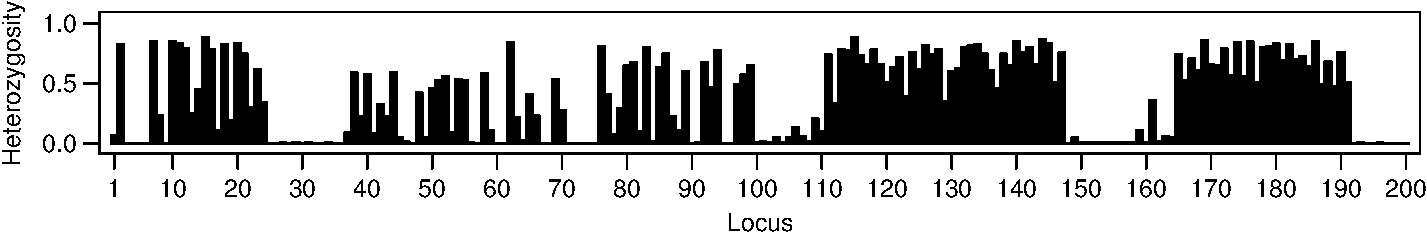
\includegraphics[width=\linewidth]{heterozygosity-plot.pdf}
\caption{The heterozygosity of each locus
  of the population before the environmental change.
  %
  Heterozygosities above 0.095 indicate
  the presence of standing genetic variation.}
\label{heterozygosity-plot}
\end{center}
\end{figure}



\section{Source of beneficial alleles}



Having established that the ancestral population
harbored abundant standing genetic variation,
I determined whether adaptation to a new environment
relied on this genetic variation or on new mutations
as a source of beneficial alleles.
%
In this study, I examined beneficial alleles
with fitness effects greater than 1\%.
%
With the ancestral population,
I started 20 new replicate populations
in a world of 1,000 cells and an environment
that rewarded for 68 different tasks
(the original nine tasks were not rewarded for).
%
As a control,
I also started another set of 20 replicate populations
where every individual had an identical genotype (i.e., isogenic),
set to the consensus sequence of the ancestral population.
%
Although the consensus genotype did not actually exist
in the ancestral population,
its fitness was 1.0070 relative to the highest fit individual
in the ancestral population
(excluding those who could immediately perform tasks),
and 1.0337 relative to the mean fitness of the ancestral population.
%
Thus, the control population was not at a disadvantage
compared to the ancestral population.
%
All other configuration settings were identical
to those used for the evolution of the ancestral population.
%
Note that the populations that started with standing genetic variation
were also allowed to get new mutations
(the mutation rate was set to 0.1 mutations per genome per generation).
%
I let these replicate populations
evolve for 10,000 updates ($\sim$~850 generations),
saving each population every 100 updates.





At the end of the runs, I found that
the populations that started with standing genetic variation
increased in mean fitness to 8.31 (7.74--8.87, 95\% bootstrap CI)
relative to the ancestral population in the new environment
(i.e., the evolved populations were 8.31 times
more fit in the new environment than the ancestral population).
%
These populations were able to perform
an average of 7.9 tasks, with a range of 5 to 10.
%
The mean number of fixed, derived alleles%
---defined as having a frequency $>$~0.95 in the evolved population
but $<$~0.95 in the ancestral population---%
was 56.25, ranging from 38 to 70.
%
Figure~\ref{allele-freq-plot} shows
the history of two allele fixation events,
one from standing genetic variation and the other from a new mutation,
that occurred in the first replicate population.
%
Of the 56.25 fixed, derived alleles,
47.8 (85\%) existed as standing genetic variation
in the ancestral population.
%
In the control populations, mean fitness increased
to 7.18 (6.62--7.76, 95\% bootstrap CI)
relative to the ancestral population.
%
The control populations were able to perform
an average of 6.7 tasks, with a range of 5 to 9.
%
The mean number of fixed, derived alleles
in the control populations was 5.15, ranging from 2 to 9.
%
It was surprising that the populations
that started with standing genetic variation
fixed 10 times more alleles than the control populations,
despite both sets of populations
having similar final fitnesses and
number of tasks performed.



\begin{figure}
\begin{center}
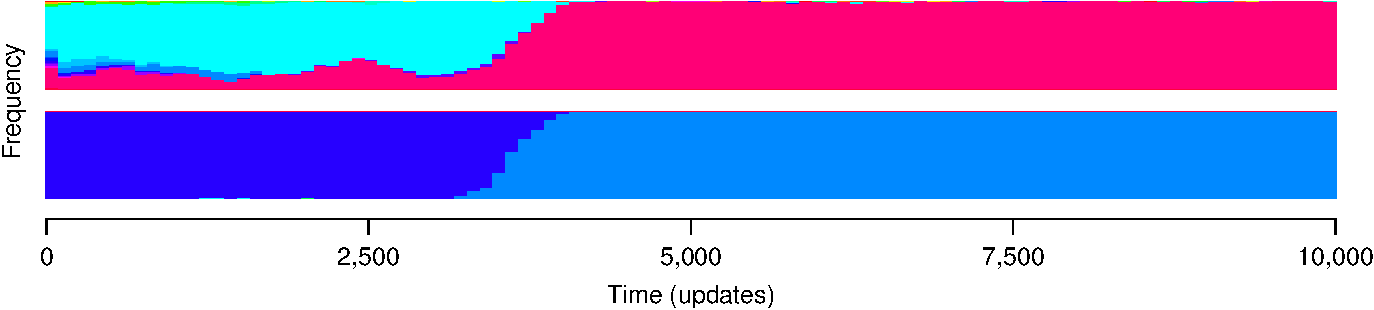
\includegraphics[width=\linewidth]{allele-freq-plot.pdf}
\caption{The frequencies of alleles through time for two loci
  in which an allele became beneficial and subsequently fixed.
  %
  In the top plot, the beneficial allele came from standing genetic variation,
  and in the bottom plot, the beneficial allele appeared as a new mutation.
  %
  Different alleles are represented by different colors.
  %
  The y-axis in each plot ranges from 0.0 to 1.0.
  %
  For interpretation of the references to color in this and all other figures, 
  the reader is referred to the electronic version of this dissertation.}
\label{allele-freq-plot}
\end{center}
\end{figure}



The finding that 85\% of fixed, derived alleles
in the populations that started with the ancestral population
existed as standing genetic variation
may indicate that most beneficial alleles came from standing genetic variation.
%
It is not clear, however, whether they were fixed
by neutral genetic drift, natural selection,
or genetic linkage and hitchhiking with beneficial alleles.
%
For example, genetic hitchhiking in Avida can occur
when alleles nearby a highly beneficial allele
rise in frequency along with the beneficial allele.
%
Hitchhiking occurs because the beneficial allele
and nearby (i.e., genetically linked) alleles
spread faster than recombination can break them apart.
%
It is also not clear at what frequency
the derived alleles first became beneficial.
%
Therefore, I developed a method to systematically
measure the fitness of individual alleles through time
and determine the frequency at which they became beneficial.





First, for each fixed, derived allele at the end of each run,
I calculated both the allele's frequency and fitness effect
every 100 updates, starting at the first update.
%
To calculate the fitness effect of an allele at the current update,
I first selected from the population the individual
with the highest fitness who had the allele.
%
I then created a clone of the individual and
substituted the allele with an alternative allele
drawn randomly from the standing genetic variation at that locus.
%
I then calculated the fitness of the individual with the allele
relative to the fitness of the individual without it.
%
If this relative fitness was greater than 1.01,
then the fitness effect of the allele ($>$~1\%)
was beneficial at the current update.
%
While testing this method, I found some cases where
the fitness effect of the allele was considered beneficial
only because the individual with the alternative allele
had unusually low fitness.
%
To reduce the frequency of such cases,
I also required that the allele be beneficial
for the individual with the second highest fitness.
%
I stopped analyzing further updates
as soon as I found the allele to be beneficial
or if it became fixed.


\begin{figure}[t!]
\begin{center}
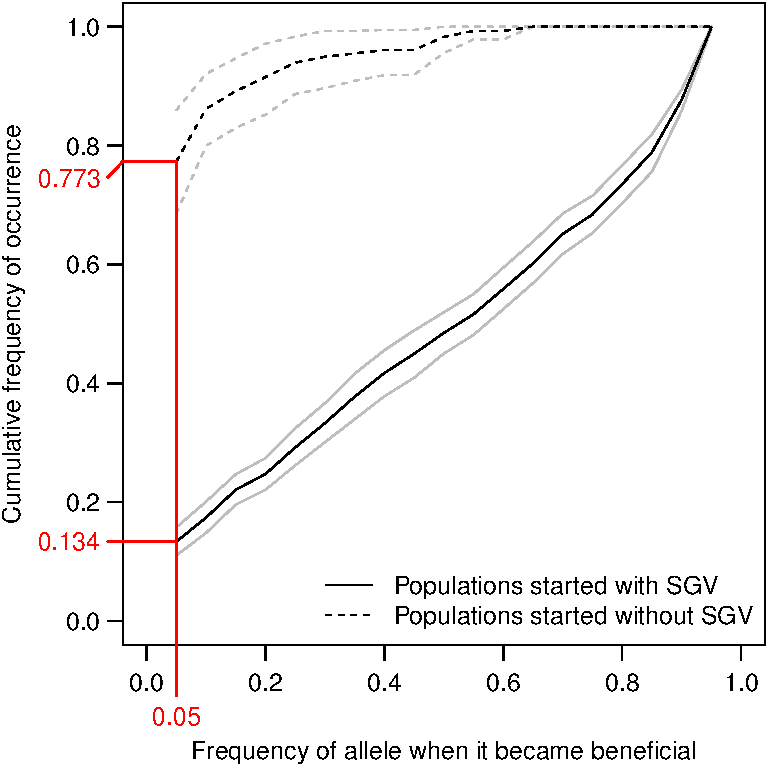
\includegraphics[width=3.5in]{cumul-freq-plot.pdf}
\caption{The cumulative frequency of fixed alleles
  that became beneficial at a specific frequency (0.05 bin size)
  for populations that started with standing genetic variation (solid lines)
  and for control, isogenic populations (dashed lines).
  %
  The gray lines indicate the 95\% bootstrap confidence interval
  around the mean of 20 replicate populations.
  %
  The red vertical line indicates the frequency
  below which alleles were considered to appear as new mutations.
  %
  The red horizontal lines indicate the proportions
  of alleles that came from new mutations
  for either type of population.}
\label{cumul-freq-plot}
\end{center}
\end{figure}


In populations that started with standing genetic variation,
I found that out of the mean 56.25 alleles that fixed,
a mean of 31.9 became beneficial at some point in their history.
%
I found that only 13.4\% of these beneficial alleles
became beneficial at a frequency $<$~0.05
(Figure~\ref{cumul-freq-plot}, lower horizontal red line);
the remaining 86.6\% became beneficial at a frequency $>$~0.05.
%
Supposing standing genetic variation comprises
alleles with frequencies $>$~0.05,
these results indicate that the majority of beneficial alleles
came from standing genetic variation.
%
In the control populations,
I found that out of the mean 5.15 alleles that fixed,
a mean of 5.1 became beneficial at some point in their history.
%
I found that 77.3\% of these beneficial alleles
became beneficial at a frequency $<$~0.05
(Figure~\ref{cumul-freq-plot}, upper horizontal red line);
the remaining 22.7\% became beneficial at a frequency $>$~0.05.
%
Therefore,
in contrast to populations that started with standing genetic variation,
the control, isogenic populations adapted mostly from new mutations,
although almost a quarter of beneficial alleles
came from standing genetic variation that arose
as populations accumulated genetic polymorphism over time.
%
Interestingly, the mean absolute (not percentage) number of new mutations
per replicate for each treatment was about the same:
4.15 (3.40--4.85, 95\% bootstrap CI) for populations started with
standing genetic variation and 3.75 (3.3--4.2) for isogenic populations.
%
This indicates that standing genetic variation did not
inhibit new mutations from being selected.





One potential concern with the above method
is that I identified beneficial alleles
based on only two genotypes that had the allele,
relative to two genotypes with alternative alleles.
%
Yet the presumed beneficial alleles as well as the alternative alleles
may not have the same fitness effect on other genetic backgrounds.
%
Thus, I implemented a second method to identify beneficial alleles
that considered more genotypes when measuring fitness effects.
%
The key difference between this method and the previous
is that in this method I selected all individuals who had the allele.
%
Then, for each of these individuals
I substituted the allele with an alternative allele
drawn randomly from the standing genetic variation at that locus.
%
Finally, I calculated the mean fitness of all individuals with the allele
relative to the mean fitness of all individuals with the allele replaced.
%
If this relative fitness was greater than 1.01,
then I considered the allele as beneficial.
%
Using this method, I found that
in populations that started with standing genetic variation,
11.5\% of alleles became beneficial at a frequency $<$~0.05;
the remaining 88.5\% became beneficial at a frequency $>$~0.05.
%
In the isogenic populations,
I found that 79.4\% of alleles became beneficial at a frequency $<$~0.05;
the remaining 20.6\% became beneficial at a frequency $>$~0.05.
%
These results are very similar to those I found with the previous method,
showing that the previous method was robust
to the number of genotypes considered when identifying beneficial alleles.



\section{Speed of adaptation}



Adaptation from standing genetic variation
should be faster than adaptation from new mutations
because beneficial alleles would be immediately available
and would be present at higher frequencies \citep{bar08}.
%
To test this prediction,
I compared the speed of adaptation between
populations that started with standing genetic variation
and those that started with isogenic individuals.
%
I re-evolved both types of populations
at the additional mutation rates (\emph{U})
of 0.01 and 0.0 (no new mutations) per genome per generation
(the original populations were run at a mutation rate of 0.1).
%
I added these new treatments because,
given that the only source of mutations
for the isogenic populations were new mutations,
the mutation rate would be an important variable
on the rate of adaptation.
%
Population size would also be an important variable
on the rate of adaptation,
but I did not investigate its effects in this study.



I found that at the 0.1 mutation rate,
the rate of adaptation for populations
that started with standing genetic variation
was significantly greater for most of the first four thousand updates
than isogenic populations,
then became less significantly so for the rest of the run
(Figure~\ref{pop-fitness-plot}A).
%
At the 0.01 mutation rate, however,
the rate of adaptation was significantly greater for the entire run
(Figure~\ref{pop-fitness-plot}B).
%
Interestingly, at the 0.0 mutation rate,
populations with standing genetic variation
continued to adapt for several thousand updates,
but, as expected, isogenic populations could not evolve
(Figure~\ref{pop-fitness-plot}C).
%
These results clearly demonstrate that
adaptation from standing genetic variation
was faster than from new mutations.
%
Yet new mutations were necessary for long-term evolution,
as shown by the fact that adaptation
from standing genetic variation without new mutations
stopped after several thousand updates.



\begin{figure}
\begin{center}
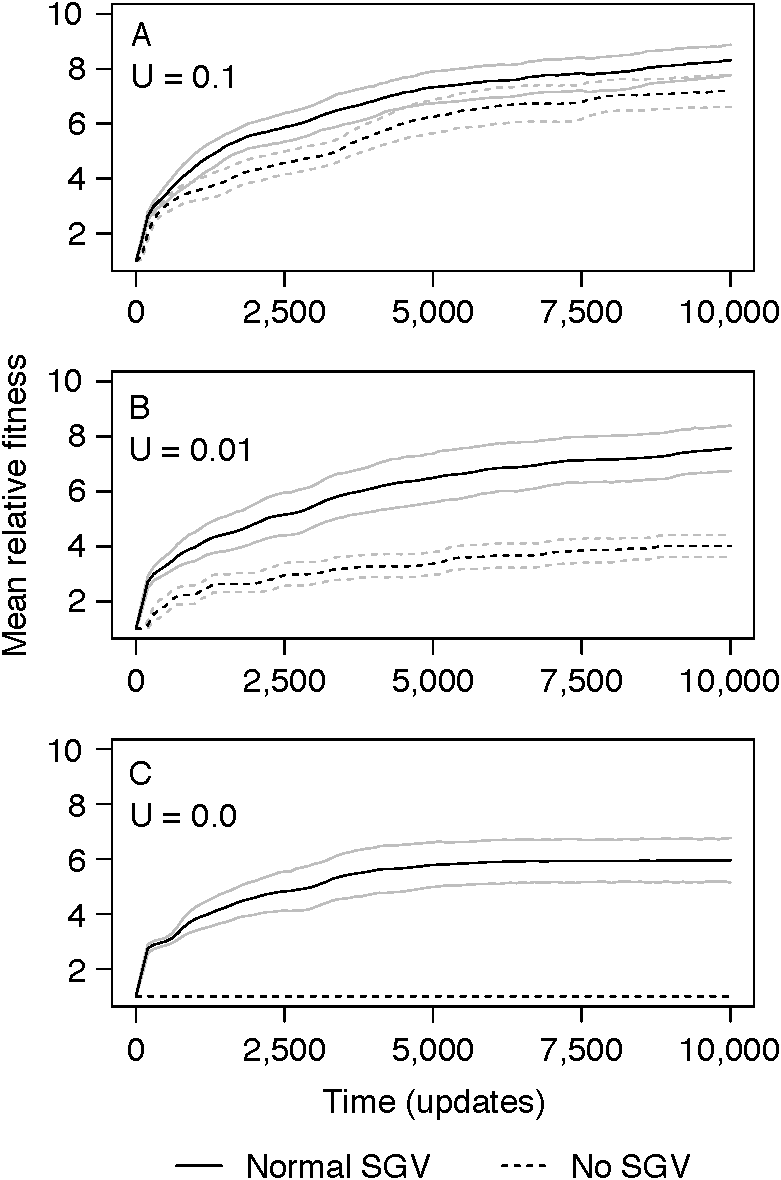
\includegraphics[width=3.5in]{pop-fitness-plot.pdf}
\caption{The mean fitnesses (relative to the ancestor)
  of populations evolved after an environmental change
  at (\textbf{A})~0.1, (\textbf{B})~0.01,
  and (\textbf{C})~0.0 mutations per genome per generation (\emph{U}).
  %
  Populations evolved starting either
  with the ancestral population (solid line),
  which contained standing genetic variation (SGV)
  or with an isogenic population based on
  the consensus sequence of the ancestral population (dashed line).
  %
  Gray lines represent the 95\% bootstrap confidence intervals
  around the mean.}
\label{pop-fitness-plot}
\end{center}
\end{figure}



\section{Fitness effect of random alleles from different sources of variation}

% - beneficial/fixed allele is present in ancestral population
%   - what was its frequency in ancestral pop?
%   - what was its effect in ancestral pop (e.g., neutral, deleterious)?
% - beneficial allele has been pre-tested:
%   - increases chance that fitness effect is advantageous

%Standing genetic variation is often
%maintained by the neutrality of alleles
%in the ancestral environment \citep{bar08}.
%%
%To test this,
%I measured the fitness of the beneficial alleles
%in standing genetic variation
%identified above in the ancestral environment.
%%
%I found that across all replicates only about 5\%
%of fitness effects were under 0.99,
%and the mean was 0.9936 (0.9847--1.003, 95\% bootstrap CI).


The distribution of fitness effects of alleles
from standing genetic variation should be different
than that of new mutations because standing genetic variation
has been `pre-tested' by selection \citep{bar08}.
%
To test this prediction,
I generated the fitness effect distribution
of alleles coming from either standing genetic variation
or new mutations, measured in the new environment.
%
First, I sampled 1,000 random (but viable)
individuals from the ancestral population
and mutated a single, random locus of each individual
to an allele drawn randomly from the standing genetic variation
(if there was any variation at that locus).
%
I also sampled another set of 1,000
individuals from the ancestral population
and mutated a single locus of each individual
to an allele drawn randomly from all 25 possible alternative alleles.
%
To prevent the possibility that these random mutations
were more deleterious only because they disrupted fixed alleles,
I ensured that the loci were drawn from the same pool
of loci that had standing genetic variation.
%
Finally, I measured the fitness of these mutants
relative to the original, unmutated individual.



I found that the mean fitness of mutants
with mutations from standing genetic variation
was 0.9994 (0.9969--1.0023, 95\% bootstrap CI).
%
The mean fitness of mutants with random mutations
was 0.9496 (0.9326--0.9665, 95\% bootstrap CI).
%
Clearly, mutations from standing genetic variation
did not have, on average, as strong deleterious effects
as random mutations.
%
To examine more closely the fitness effects
of mutations from the two sources,
I categorized each mutation based on
the mutant's relative fitness (Table~\ref{mutant_fitness_table}).
%
Alleles from standing genetic variation were mostly neutral,
whereas new mutations were more likely to be lethal or deleterious.
%
Interestingly, new mutations were also more likely
to be strongly beneficial than alleles from standing genetic variation,
yet in the analysis where I determined the source of beneficial alleles,
I found that most beneficial alleles came from standing genetic variation.
%
This discrepancy may indicate that although alleles
from standing genetic variation were not beneficial alone,
combinations of these alleles brought together
by recombination provided the benefits.
%
The finding that alleles from standing genetic variation
were less deleterious on average than random mutations
support the hypothesis that standing genetic variation
has been pre-tested by selection.



\begin{table}
\begin{center}
\begin{tabular}{|l|c|c|}
\cline{2-3}
\multicolumn{1}{l}{} & \multicolumn{2}{|c|}{Source of mutation} \\
\hline
Fitness effect & SGV & Random \\
\hline\hline
Lethal & 0 & 58 \\
Strongly deleterious & 3 & 5 \\
Mildly deleterious & 186 & 345 \\
Nearly neutral & 729 & 520 \\
Mildly beneficial & 81 & 67 \\
Strongly beneficial & 1 & 5 \\
\hline
\end{tabular}
\caption{The number of single mutants (out of 1,000),
  categorized by the mutation's source and fitness effect ($w$):
  lethal ($w =$~0),
  strongly deleterious (0~$< w \le$~0.99),
  mildly deleterious (0.99~$< w \le$~0.999),
  neutral or nearly neutral (0.999~$<$ $w \le$~1.001),
  mildly beneficial (1.001~$< w \le$~1.01),
  and strongly beneficial ($w >$~1.01).}
\label{mutant_fitness_table}
\end{center}
\end{table}



The above analysis was based on randomly generated mutants
of the ancestral genotypes (i.e., at the beginning of the experiments),
but it would also be interesting to know
the fitness effect of beneficial alleles that actually fixed.
%
This information was already calculated
as part of determining the moment at which alleles
became beneficial because it was used to determine
whether alleles had achieved a fitness $>$~1.01 (using the first method).
%
For populations that had evolved under standing genetic variation,
the mean fitness of a genotype with a beneficial allele
at the moment at which it became beneficial
(relative to a genotype without the beneficial allele)
was 1.54 (1.48--1.60, 95\% bootstrap CI).
%
For isogenic populations,
this mean fitness was 1.47 (1.37--1.59, 95\% bootstrap CI).
%
Although the mean fitness effect of beneficial alleles
for the standing genetic variation treatment
was slightly higher than the isogenic treatment,
they were not significantly different.
%
The maximum relative fitness for a genotype with a beneficial allele
for the standing genetic variation treatment (7.05)
was higher than that for the isogenic treatment (4.50).





\section{Discussion}


% every statement I make must be supported by my results,
% the results of others, or authoritative statements
% based on the results of others
% - the reference must be the one from which the original
%   information came, not from a paper that used that information
%   to make further arguments

% Start with the main point: source of beneficial mutations,
% using the same words I used in the Introduction


I have shown that in populations of digital organisms
adapting to a new environment,
the major source of beneficial alleles
was standing genetic variation, not new mutations.
%
My findings are supported by
selection experiments and observational studies
of biological populations.
%
Selection experiments have shown that
adaptation can occur by changes in allele frequencies
of standing genetic variation in the initial populations
\citep[e.g.,][]{fed97,sca09,teo09}.
%
Observational studies of natural populations
have found that alleles correlated with adaptive traits
were also present in the ancestral population
\citep[e.g.,][]{col05,myl05}.
%
% (Examples of new mutations?)
%
In biological organisms, however,
it is very difficult to measure
the fitness effects of individual alleles,
which is necessary to determine whether
an allele fixed due to selection.
%
Another problem, specific to studies of natural populations,
is that the ancestral population is unavailable%
---the closest one can get is the extant population
from which a subpopulation founded a new environment---%
and therefore it is often unknown
whether a beneficial allele existed as standing genetic variation.
%
The use of digital organisms allowed me to track
individual alleles through time
and determine the frequency at which they became beneficial.

% Something about generalization
%I show that in a general evolving genetic system,
%standing genetic variation provides most of the beneficial alleles
%to a population adapting to a new environment.



When alleles from standing genetic variation became beneficial,
their starting frequency ranged from the minimum of 5\%
to the maximum of 95\% (Figure~\ref{cumul-freq-plot}).
%
In experimental studies of biological organisms,
high starting frequencies ($>$~50\%) are not uncommon
\citep[e.g.,][]{fed97,sca09}.
%
In natural populations, however,
starting frequencies have tended to be much smaller,
such as in the study by \citet{col05},
where the starting frequency of an adaptive allele
was between 0.2\% and 3.8\% in the ancestral population.
%
One possible reason for this discrepancy
is that natural populations may be under stronger selective pressures
than experimental populations \citep{ell08},
so the fitness effects of alleles in natural populations
tend to be more deleterious and therefore maintained at low frequencies.
%
Of course, allele frequency data for adaptive alleles
in natural populations is scarce,
so more research in natural populations
should determine the frequencies at which alleles
from standing genetic variation become beneficial.



Adaptation should be faster if most beneficial alleles
came from standing genetic variation
than if they came from new mutations \citep{bar08}.
%
I found this to be the case in digital organisms
if the mutation rate was low enough (Figure~\ref{pop-fitness-plot}).
%
In fact, when no new mutations were allowed,
adaptation by standing genetic variation continued
for several hundred generations,
whereas no adaptation occurred in isogenic populations.
%
Still, the importance of new mutations
for long-term evolution was shown by the fact
that adaptation stopped eventually
when no new mutations were allowed.
%
Although there are no empirical studies
testing the speeds of adaptation,
where beneficial alleles may come from
either standing genetic variation or new mutations,
my results are supported theoretically \citep{her05}.
%
There are two reasons that adaptation
from standing genetic variation should be faster
than adaptation from new mutations:
beneficial alleles are both readily available
and present at higher frequencies than alleles
from new mutations \citep{bar08},
which must overcome drift because they start at lower frequencies.
%
Future experiments should be able to quantify
the relative contribution of these two causes.



Although not examined in detail in this study,
the population size and mutation rate can affect the relative contributions
of standing genetic variation and new mutations during adaptation.
%
For example, a sudden decrease in population size (i.e., a bottleneck)
will reduce both the amount of standing genetic variation
and the number of new mutations that appear each generation.
%
In this case, standing genetic variation
will still have an advantage over new mutations---%
especially for alleles of weak fitness effect---%
because weak effect alleles introduced by new mutations
are easily lost due to genetic drift \citep{her05}.
%
For large effect alleles,
standing genetic variation will have a reduced advantage
because large effect alleles are less likely to be lost
even if they are introduced as new mutations \citep{her05}.
%
In my experiments, mutations that allowed organisms
to perform new tasks were of large effect
(the default configuration in Avida),
but future studies should experiment with weaker beneficial alleles.
%
In a large population or high mutation rate,
new mutations would become more important
because large-effect mutations would appear more frequently.



Because alleles from standing genetic variation
have had a potentially long history in an evolving population,
their fitness effects in a new environment
have been predicted to be less deleterious
than random mutations \citep{bar08}.
%
On average, I found that
standing genetic variation was effectively neutral
(fitness effect of 0.0006),
whereas random mutations were strongly deleterious
(fitness effect of 0.0504).
%
Alleles from standing genetic variation can therefore linger in a population,
increasing the chance for them to become beneficial
after an environmental or genetic change.
%
Random mutations, on the other hand, are on average deleterious
and are thus more easily eliminated by selection.
%
In biological populations,
the mean fitness effect of random mutations
was found to be 0.48 in RNA viruses \citep{san04},
0.12 in \emph{C. elegans} \citep{vas00},
and 0.22 in yeast \citep{zey01}.
%
There are no measurements of the fitness effects
of alleles from standing genetic variation
in a biological population in a new environment.



For strongly beneficial mutations (i.e., fitness effect $>$~1\%),
I found that random mutations were more likely to be beneficial
than alleles from standing genetic variation
in the new environment (Table~\ref{mutant_fitness_table}).
%
It may thus seem counter-intuitive that
most beneficial alleles during adaptation
came from standing genetic variation.
%
I hypothesize that it was the combination of many alleles
from standing genetic variation that provided the benefits,
and together these epistatically related alleles rose to fixation.
%
Adaptation that requires many alleles working together
is known as `polygenic adaptation' \citep{pri10},
although fixation of alleles is not always necessary.
%
In fact, \citet{pri10} hypothesize that if
adaptation occurs from standing genetic variation,
polygenic adaptation is likely.



In summary,
this study has shown the importance of standing genetic variation
in populations of digital organisms adapting to a new environment.
%
That is,
(1) most beneficial alleles came from standing genetic variation
rather than from new mutations,
(2) populations that started with standing genetic variation
adapted faster than populations that started with identical genotypes,
and (3) the fitness effects of alleles from standing genetic variation
were less harmful than new mutations.
%
Because digital organisms evolve by the same
processes of natural selection and genetic drift
that biological populations also experience,
I suspect that the above points are also true for biological populations.
%
A hypothesis that arose from this study
was that standing genetic variation together with recombination
may give rise to combinations of alleles that together are beneficial.
%
Future work should test whether this additional advantage is true,
thereby highlighting the importance of sexual recombination
and standing genetic variation in evolving populations.


% consider plotting the substitutions through time

% paragraph on limitations of Avida

% paragraph on future work

% say something about cryptic genetic variation

% undoubtedly, more loci are important (not just fixed),
% as has been observed in literature, but fixed gave us a starting point

% Colosimo et al - Eda: 0.2% and 3.8%

% FRIGIDA - 40% - 60% (artificial)

% Feder et al 1997:
% hawthorns are the ancestral host of R. pomonella
% - so hawthorn race of pomonella is ancestral pop of apple pomonella?

% Teotonio: 70% of SNPs had freqs > 5% in control/ancestral pops
% - allele frequencies didn't change much although adaptation occurred

% Begin with I found and THEN compare them to other studies

% Always end with a conclusion, something drawn out of my results,
% but a conclusion can be a summary of the issue incorporating my findings,
% a recommendation, speculation (that could be used to form a new hypothesis),
% a new principle, or that there isn't enough evidence to form a conclusion
% - the conclusion should be a simple, easy to read sentence

% ideas developed from the results
% practical application or contribution to general thinking of my discipline

% start paragraphs with a brief summary of what's to come,
% and include a transition from the previous paragraph

% organize ideas in order of importance
% 1 - relevant to original hypothesis, accept/reject
% 2 - relevant, but not conclusive; need more study
% 3 - not relevant to original hypo, but based on results; new & interesting
% 4 - anything else -- excise from discussion

% What are the limitations of my study?

% What remains to be done, suggest additional research
% What more would I like to know?

% Why is my claim significant?
% What are its consequences?
% Any new significance not mentioned in the Intro?
% (but careful not to make it the main point)



% Things to consider:

% New mutations have to be important for long-term evolution
% - it could be that mutations serve to generate SGV,
%   but evolution mostly happens from SGV
%   - would have to track where mutations come from
%     in the mutation-only treatment

% I find that ANOTHER reason sgv is good for adaptation
% is that beneficial COMBINATION of alleles are already present,
% whereas mutation typically happens one-by-one

% Future work: How does sgv change through time
%   for those that started with sgv and those that didn't.

% Future work: more generations, long-term

\end{doublespace}

\begin{lit_cited}
\end{lit_cited}

\bibliographystyle{apalike}
\bibliography{sgv}

\begin{doublespace}

\chapter{The probability of compensatory adaptation in digital organisms}
\label{chap:comp_rate}



\section{Introduction}

Deleterious mutations may accumulate in a population
through various mechanisms: genetic drift \citep{lan94,lyn95},
hitchhiking with beneficial mutations \citep{chu11},
transient environmental changes \citep{bjo00},
and selfish genetic elements \citep{pre10}.
%
In these deteriorated populations, new beneficial mutations
may arise and restore the fitness of the population.
%
These beneficial mutations, however, may not have been beneficial
in the absence of the accumulated deleterious mutations.
%
In other words, their effect may epistatically depend
on the current genetic background, and without the deleterious mutations,
they may have had no benefit or even have been deleterious.
%
These beneficial mutations are known as `compensatory mutations,'
and the process by which compensatory mutations recover fitness
is known as `compensatory adaptation.'
%
Experimental evolution studies have observed compensatory adaptation
\citep{har96,bur99,moo00,lev00,mai02,est03,est11}.



Understanding compensatory adaptation has practical applications to society,
such as the conservation of threatened or endangered species
and the antibiotic resistance of pathogenic bacteria.
%
Theoretical work has shown that small populations
($<$~100 individuals) or populations that have undergone bottlenecks
will readily fix deleterious mutations \citep{whi03}.
%
There is the risk that such populations will go extinct \citep{lyn95,lan94},
unless compensatory adaptation could help them recover.
%
Bacteria susceptible to an antibiotic may acquire resistance mutations
in the presence of the antibiotic, but such mutations
are often deleterious in the absence of the antibiotic \citep{sch97,lev00}.
%
The hope for combating resistant bacteria was to remove the antibiotic,
so that a competitively superior susceptible strain
would evolve through reversion.
%
Resistant bacteria, however, may instead acquire compensatory mutations
that remove this fitness deficit while retaining their resistance
\citep{sch97,lev00,bjo00,mai02,pau07,per10}.
%
In fact, because compensatory mutations often depend on
the deleterious mutations already present,
reversion and susceptibility become increasingly difficult.



Experimental studies have found that compensation, rather than reversion,
often occurs, but reversion is sometimes present or inferred
\citep{bur99,san05,mai02}.
%
The reason that reversion is rare has been argued to be that
compensatory mutations are much more frequent than revertant mutations
(i.e., there is only one way to revert, but many ways to compensate)
\citep{lev00,whi03,san05}.
%
One might expect, however, that once the revertant mutation appears
it would most likely fix because its fitness recovery is 100\%
(i.e., its selective value would be higher than that of compensation).
%
However, epistasis is common in organisms, and the possibility
exists that once a few compensatory mutations arise and fix,
the revertant mutation will not provide its full benefits because
it would interact negatively with compensatory mutations.
%
This possibility has been observed experimentally \citep{sch97,lev00}.
%
The conflict between compensatory and reversion is a complicated
interaction involving, at least, the initial fitness of the mutant,
population size, and mutation rate.
%
Here I examine the effect of these factors one by one
on the probability of compensation vs. reversion.



The initial fitness is important because, primarily, it will determine
the fitness effect of the reversion when it appears,
assuming this fitness has not changed because of compensatory mutations.
%
It is also important because the number of compensatory mutations
may be different, given that it is expected that there will be more ways
to compensate the lower the fitness of the mutant.
%
The population size is important because it partly determines
how many mutations arise each generation.
%
Larger populations will increase both the frequency of compensatory mutations
and that of reversion, and studies have confirmed
that reversion occurs more frequently in large populations \citep{bur99}.
%
Like population size, mutation rate also affects the frequency
in which mutations arise.
%
However, greater mutation rates increase the chance that double-mutants appear,
such that a revertant mutation may arise with a deleterious mutation
and thus cancel out its benefit.



In this study, I used experimental evolution \emph{in silico}
using the artificial life system Avida \citep{ofr04}
(see p. \pageref{sec:avida})
to examine the evolutionary dynamics of compensatory adaptation.
%
The use of digital organisms allowed us to answer questions
that would be difficult even with microbial organisms.
%
With digital organisms,
one can observe hundreds of generations in a few minutes,
conduct hundreds of replicate experiments,
easily manipulate genomes,
and accurately measure fitness.
%
Although the system I used is artificial, it has been shown that
several biological phenomena emerge naturally in Avida \citep{wil02,ada06}.
%
Digital organisms improve on mathematical models of adaptation
because in this system traits are complex,
involving multiple loci and epistatic interactions among alleles \citep{len99}.



In these experiments, populations of mutants
with a single deleterious mutation
were allowed to evolve for $\sim$~850 generations.
%
I first estimated the availability of compensatory mutations
depending on the initial fitness of the mutant.
%
Then, I examined the effect of three variables---%
the initial fitness of the mutant, the population size,
and the mutation rate---%
on the probability of compensation vs. reversion.
%
From these experiments, I hope to learn the conditions under which
compensation or reversion are likely to occur.
%
I hope to understand whether compensatory mutations
could change the window of opportunity for reversion,
either because compensatory mutations arise much more frequently
or because negative epistasis is common.



\section{Results}

I evolved two ancestral populations of digital organisms (see Methods),
each composed of 10,000 individuals,
to the default environment for 500,000 updates ($\sim$~40,000 generations).
%
Each individual was haploid, reproduced asexually,
had a genome length of 200, and had a mutation rate of 0.1
per genome per generation.
%
Both ancestral populations had evolved long enough to fully adapt
and population fitness had stabilized for thousands of generations;
therefore, I consider each of these populations
to be near their respective optimal fitness for this environment.
%
Although at the phenotypic level both populations
had evolved to similar fitnesses,
at the genomic level, they exhibited only 13.5\% identity,
meaning that they represent independent experimental organisms.
%
The consensus sequence of these two ancestors served
as the ancestral genotypes for subsequent experiments.
%
For each of these ancestral genotypes,
I identified five sets of two mutants,
each pair with approximately a fitness of either
0.1, 0.3, 0.5, 0.7, and 0.9 relative to the ancestor,
for a total of 20 mutant genotypes.



\subsection{Frequency of compensatory mutations}

Before I started the experimental evolution of mutants,
I confirmed in digital organisms theoretical and empirical expectations
about the availability of compensatory mutations in other organisms:
there should be more compensatory mutations the lower the initial fitness
(i.e., there are more ways to compensate the lower your fitness).
%
This expectation has been made theoretically from extreme value theory,
where the tail of any distribution
(in this case, the distribution of beneficial mutations),
follows the same extreme value distribution \citep{orr02},
so the higher the fitness, the fewer beneficial mutations that are found.
%
Empirical studies \citep[e.g.,][]{ele98,bur99} have also shown
that populations with deleterious mutations readily gain
more beneficial mutations than fit populations \citep{whi00}.
%
To test this hypothesis, I introduced every possible single mutation
on each mutant and counted the number that were fully or partially compensatory
(i.e., fitness increased in the presence of the deleterious mutation).
%
I confirmed that in digital organisms, as in biological,
there were more compensatory mutations available in the mutants
with low fitness than in those with high fitness (Figure~\ref{fig:comp_avail}).
%
These results also confirm that there are more compensatory mutations
than reversion (which is always exactly one),
corroborating suggestions that compensation is more likely than reversion
\citep{mai02}.



% Update picture so that I choose either A or B (no need to have both,
% but mention in the text), most importantly, change the points so that
% they represent mutant replicates, not ancestral replicates;
% figure B should be the second ancestor.
\begin{figure}
\begin{center}
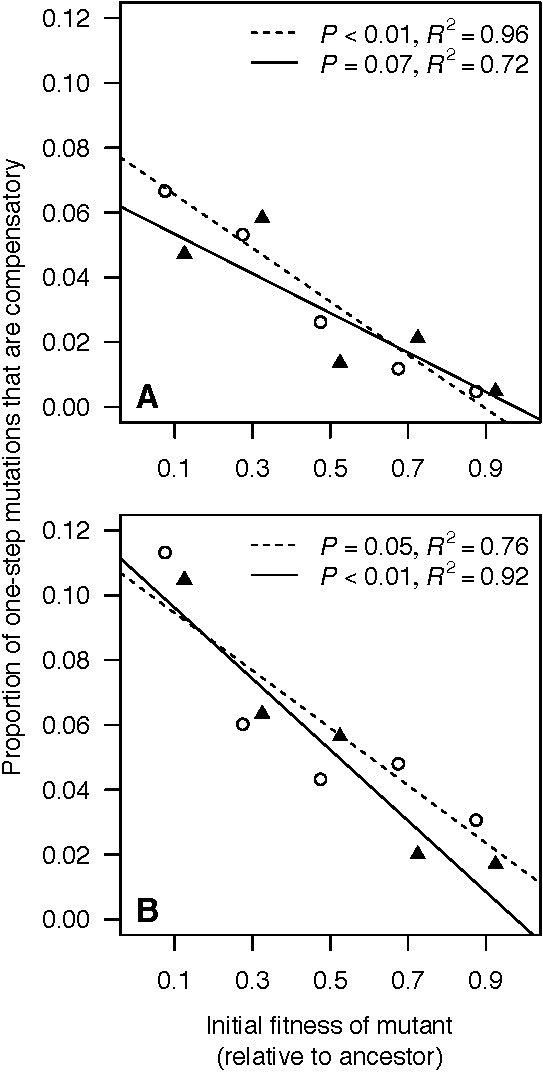
\includegraphics[width=3.5in]{comp-avail.pdf}
\end{center}
\caption{{\bf Proportion of one-step mutations that are compensatory.}
  (A) Ancestor 1 and (B) Ancestor 2.
  %
  Open circles ($\ocircle$) and dashed lines
  represent the first mutant replicate
  while solid triangles ($\blacktriangle$) and solid lines
  represent the second mutant replicate.
  %
  Error bars are the 95\% confidence interval of the mean.}
\label{fig:comp_avail}
\end{figure}



\subsection{Effect of initial fitness of mutant}

% Perhaps have suppl. figures showing fitness increase
I evolved these 20 mutant genotypes independently
for 10,000 updates ($\sim$~850 generations)
under the same environment as the original ancestors.
%
For each genotype, the starting population
was composed of 1,000 genetically-identical individuals,
and the experimental evolution for each genotype was replicated 100 times.
%
I found that the probability of compensatory adaptation
declined with the fitness of the initial mutant
(Figures \ref{fig:W_comp}A and \ref{fig:W_comp}B).
%
In contrast, the probability of reversion
increased with the fitness of the initial mutant
(Figures \ref{fig:W_comp}C and \ref{fig:W_comp}D).
%
Note that because in some runs the fitness values decreased or did not change,
the addition of compensatory and reversion probabilities
did not always add up to 100.
%
Note also that there is a difference in the probability of compensation
for W = 0.9 between the first and second ancestor.
%
The reason for this difference appears to be that
for the first ancestor, neither compensation nor reversion
occur---the population does not change fitness.
%
This is may be due to the fact that there are few compensatory mutations
available for ancestor 1 for W = 0.9 (see Figure \ref{fig:comp_avail}).



\begin{figure}
\begin{center}
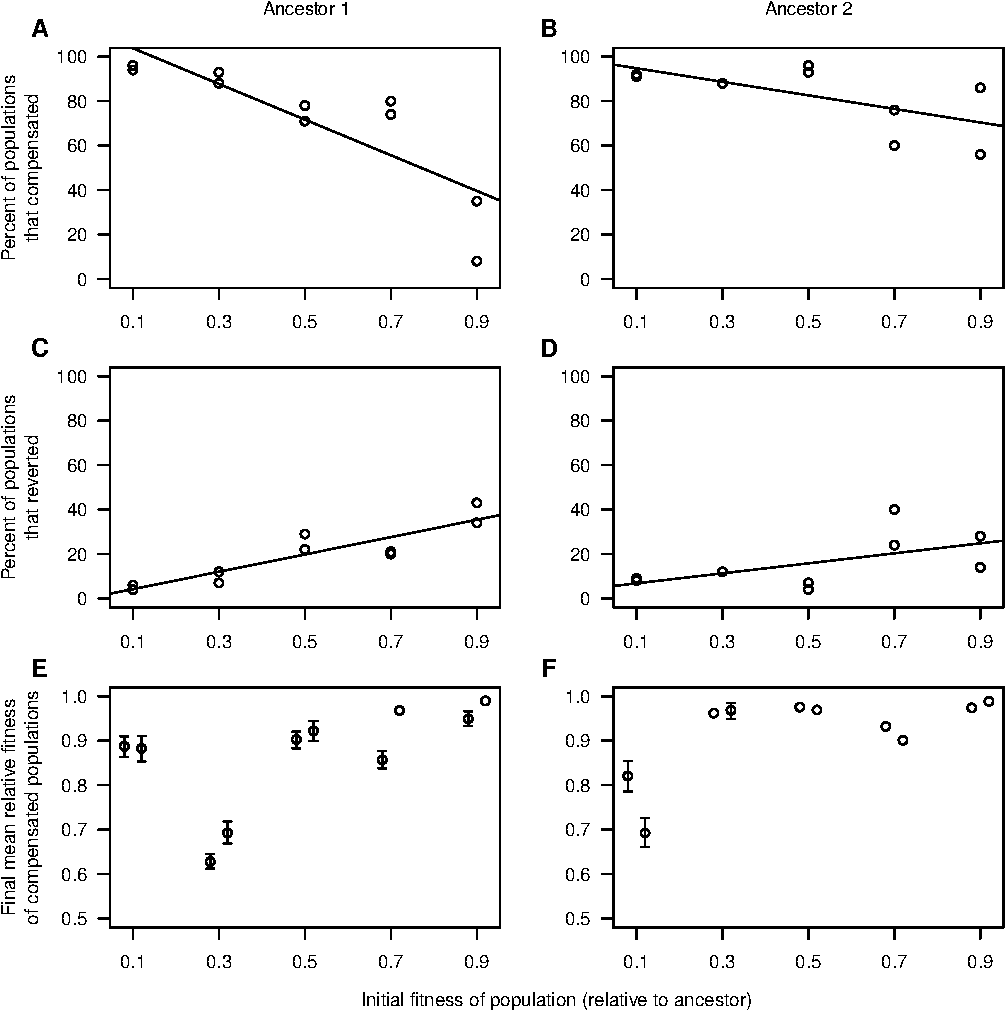
\includegraphics[width=\linewidth]{effect-W.pdf}
\end{center}
\caption{{\bf Effect of initial fitness on compensation.}
  Top figures: The proportion of runs that fully or partially compensated
  for (A) ancestor 1 (line is best fit linear model, $P =$~0.002) and
  (B) ancestor 2 ($P =$~0.043).
  Middle figures: The proportion of runs that reverted
  for (C) ancestor 1 ($P <$~0.001) and (D) ancestor 2 ($P =$~0.072).
  %Bottom figures may be irrelevant -- consider eliminating
  Bottom figures: The proportional increase in fitness for compensatory runs
  for (E) ancestor 1 and (F) ancestor 2.}
\label{fig:W_comp}
\end{figure}



There are several reasons that would explain why compensation
is higher than reversion the lower the fitness of the original mutant.
%
It is important to note that the probability
that a reversion fixes is determined by its selective advantage,
which itself depends on the fitness of the population
and on whether there is negative epistasis with current mutations.
%
The fitness of the population is initially set by the treatment
but it changes during the experiment depending on the speed of compensation.
%
The speed of compensation is directly affected by
the initial fitness of the population: the lower the initial fitness
the faster the population compensates and thus increases in fitness.
%
Negative epistasis is an intrinsic property of mutations,
but the total amount of negative epistasis is affected
by the number of mutations present when the reversion arrives.
%
This number of mutations depends on the speed of compensation
and the rate of compensatory mutations,
both of which are partly determined by the initial fitness of the population.
%
Therefore, there are both direct and indirect ways
in which the lower the initial fitness of the population
the lower the probability that a reversion fixes.



If negative epistasis was present,
the expectation is that reversion would stop being beneficial
as mutations fixed in the population.
%
The sooner reversions stopped being beneficial
the stronger that negative epistasis is with other mutations.
%
To test whether negative epistasis may have contributed in
preventing reversions from spreading in the evolving populations,
I calculated the number of generations in which a reversion
stopped being beneficial in populations that did not eventually revert.
%
First, I reverted the initial mutation to the ancestral state
for every individual in the population at each update saved
(every 100 updates or $\sim$~8.5 generations).
%
I then calculated the mean fitness of this population
relative to the mean fitness of the original population.
%
Finally, starting at the first update and continuing sequentially,
I tested whether the mean relative fitness of the reverted population
was less than 1.001; if so, reversion was no longer beneficial at this update.
%
I found that reversion stopped being beneficial sooner
at large-effect initial mutations than at small-effect initial mutations
(Figure~\ref{fig:first-update-rev-bad-W}),
indicating that negative epistasis was strongest for large-effect mutations.



\begin{figure}
\begin{center}
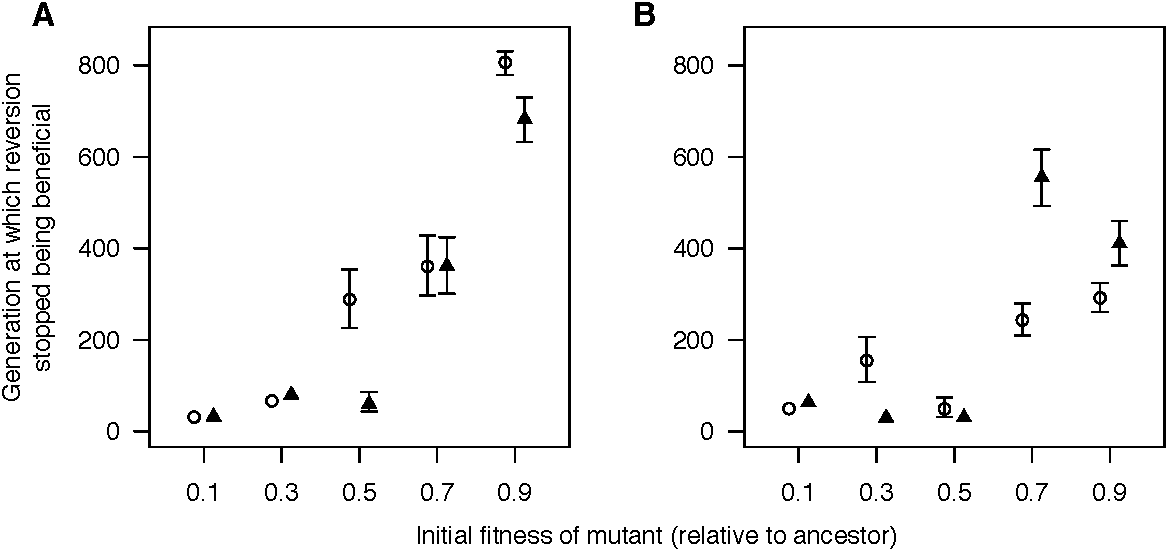
\includegraphics[width=3.5in]{first-update-rev-bad-W.pdf}
\end{center}
\caption{{\bf Generation at which reversion stopped being beneficial
  at various initial mutant fitness effects.}
  %
  (A)~Ancestor~1 and (B)~Ancestor~2.
  %
  Open circles ($\ocircle$) and dashed lines
  represent the first mutant replicate
  while solid triangles ($\blacktriangle$) and solid lines
  represent the second mutant replicate.
  %
  Error bars are the 95\% confidence interval of the mean.}
\label{fig:first-update-rev-bad-W}
\end{figure}



As I noted before, however, the overall amount of negative epistasis
is proportional to the number of mutations accumulated.
%
Because populations that start with lower fitness adapt faster
than populations with higher fitness, they accumulate more mutations
and therefore have greater total negative epistasis.
%
In this case, negative epistasis is explained by the speed
at which compensation proceeds,
not by an intrinsic difference in negative epistasis
among treatments (i.e., initial fitness of mutant).
%
To determine whether the amount of negative epistasis
is different among treatments by accounting for the different
speeds at which compensation occurs,
I determined the number of mutations accumulated per treatment
at which reversion stopped being beneficial.
%
By examining the number of mutations accumulated
rather than the number of generations that have elapsed,
I controlled for the varying number of mutations
that accumulated through time for each treatment.
%
I still found that reversion stopped being beneficial sooner
for large-effect initial mutations than for small-effect initial mutations
(Figure~\ref{fig:first-mut-rev-bad-W}),
indicating that negative epistasis was strongest for large-effect mutations.



\begin{figure}
\begin{center}
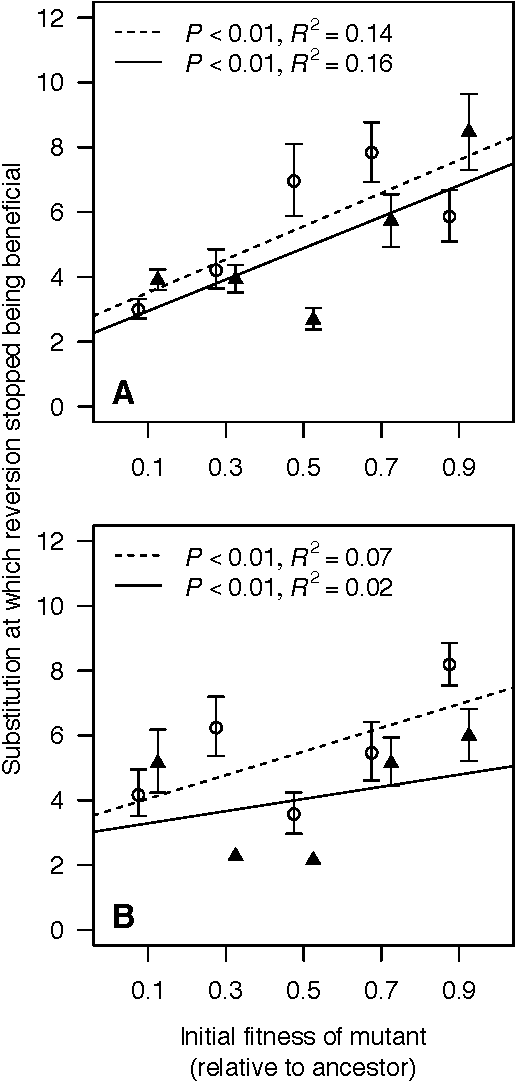
\includegraphics[width=3.5in]{first-mut-rev-bad-W.pdf}
\end{center}
\caption{{\bf Substitution at which reversion stopped being beneficial.
  at various initial mutant fitness effects.}
  %
  (A)~Ancestor~1 and (B)~Ancestor~2.
  %
  Open circles ($\ocircle$) and dashed lines
  represent the first mutant replicate
  while solid triangles ($\blacktriangle$) and solid lines
  represent the second mutant replicate.
  %
  Lines are linear regressions for each mutant replicate.
  %
  Error bars are the 95\% confidence interval of the mean.}
\label{fig:first-mut-rev-bad-W}
\end{figure}



To further show that negative epistasis contributed
to shortening the window of opportunity for reversion,
I estimated the time at which a reversion must appear
in order to eventually reach fixation
with and without negative epistasis (see Methods).
%
These estimates were calculated using Markov chain simulations
and the known probability of reversion and selective coefficient through time.
%
I then compared these results with runs in which reversion did occur.
%
If the estimates calculated in the presence of negative epistasis
match the actual runs better than the estimates calculated without epistasis,
then I can be sure that negative epistasis
was an important contributor to slowing down the rate of reversion.
%
Indeed, I found that the actual runs matched the estimates
that were calculated in the presence of negative epistasis
(Figure~\ref{fig:expected-rev}).
%
Without negative epistasis, a reversion may appear late in evolution
and still reach fixation because its selective benefit lasts longer.
%
With epistasis, however, the window of opportunity was small,
so a reversion must appear early on if it will fix,
which was exactly what I observed in the actual runs that reverted.



\begin{figure}
\begin{center}
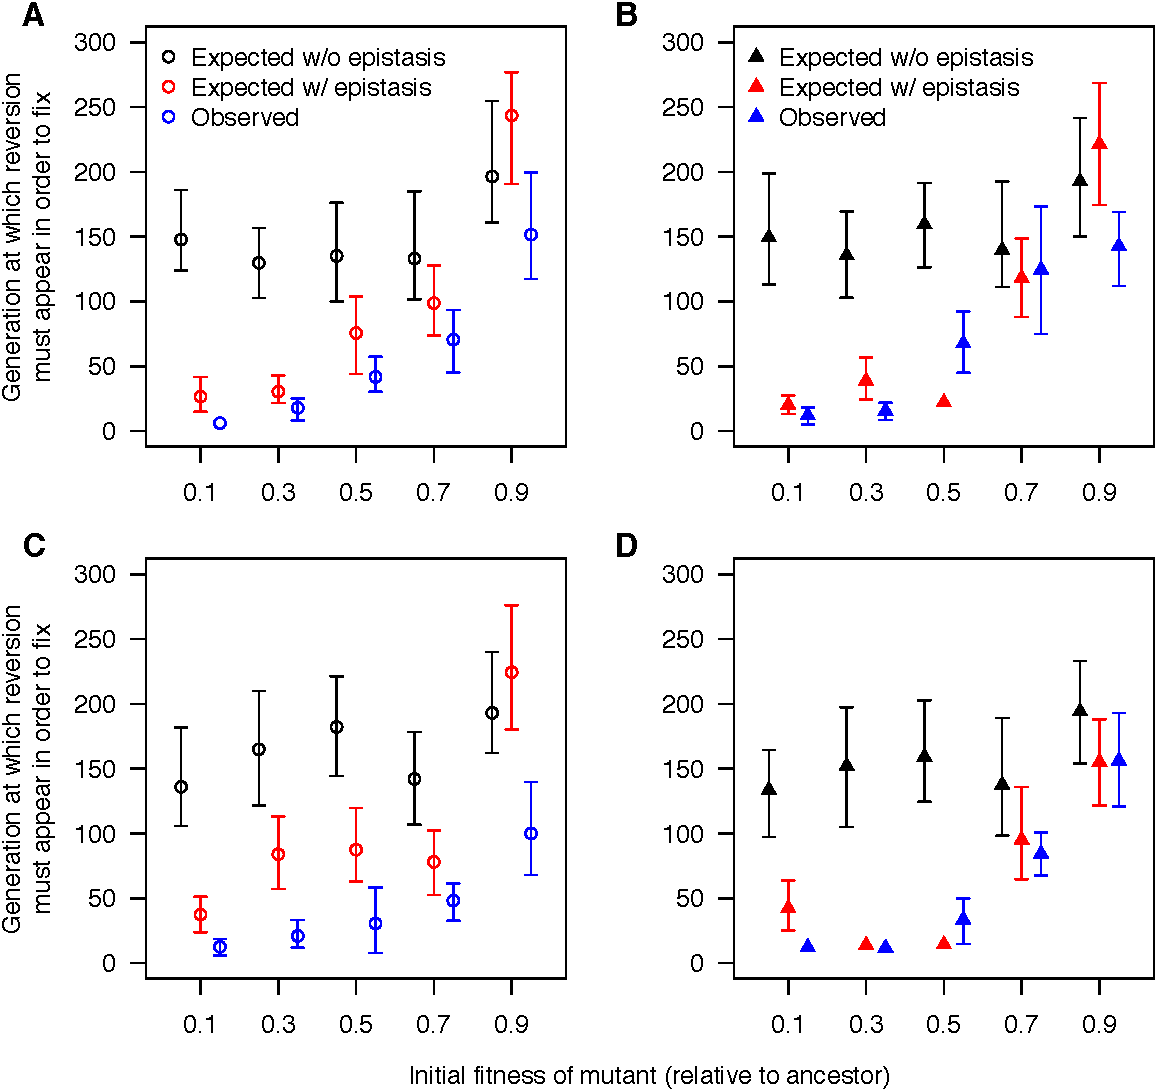
\includegraphics[width=\linewidth]{expected-rev.pdf}
\end{center}
\caption{{\bf Generation at which reversion must appear in order to fix.}
  (A)~Ancestor~1, Mutant~1, (B)~Ancestor~1, Mutant~2,
  (C)~Ancestor~2, Mutant~1, and (D)~Ancestor~2, Mutant~2.
  %
  Open circles ($\ocircle$) represent the first mutant replicate
  while solid triangles ($\blacktriangle$)
  represent the second mutant replicate.
  %
  Error bars are the 95\% confidence interval of the mean.}
\label{fig:expected-rev}
\end{figure}



I have learned that the probability of compensation and reversion
depends on the probability of finding these different kinds of mutations.
%
I should therefore expect that the population size,
which increases the total number of mutants available,
should play an important role in the probability of compensation.
%
I know that reversion is more likely to occur if it appears early
because compensatory mutations have not had an opportunity
to decrease the fitness effect of reversion
and because they have not incurred negative epistasis with reversion.
%
In large populations, the opportunity for a reversion to appear early
is higher, thus larger populations should revert more often.
%
I next examine the effect of population size on the probability
of compensation and reversion.



\subsection{Effect of population size}

I evolved the four mutants with relative fitness of 0.5
under four population sizes each: 10, 100, 1,000, and 10,000.
%
Each of these 16 experiments was replicated 100 times,
starting with a full population of genetically-identical individuals,
and evolved for 10,000 updates ($\sim$~850 generations).
%
The mutation rate was set to 0.1 mutations per generation for each experiment.
%
I found that the probability of compensatory adaptation
was highest at population sizes of 100 and 1,000
but lowest at the extremes of 10 and 10,000
(Figures \ref{fig:N_comp}A and \ref{fig:N_comp}B).
%
The probability of reversion was highest at population size of 10,000
(Figures \ref{fig:N_comp}C and \ref{fig:N_comp}D).
%
The final fitness of compensated populations
was higher the higher the population size
(Figures \ref{fig:N_comp}E and \ref{fig:N_comp}F).
%
Thus, although intermediate population sizes
had the highest probability of compensating,
they did not have the highest final fitness;
populations with size of 10,000 had the highest fitness.



\begin{figure}
\begin{center}
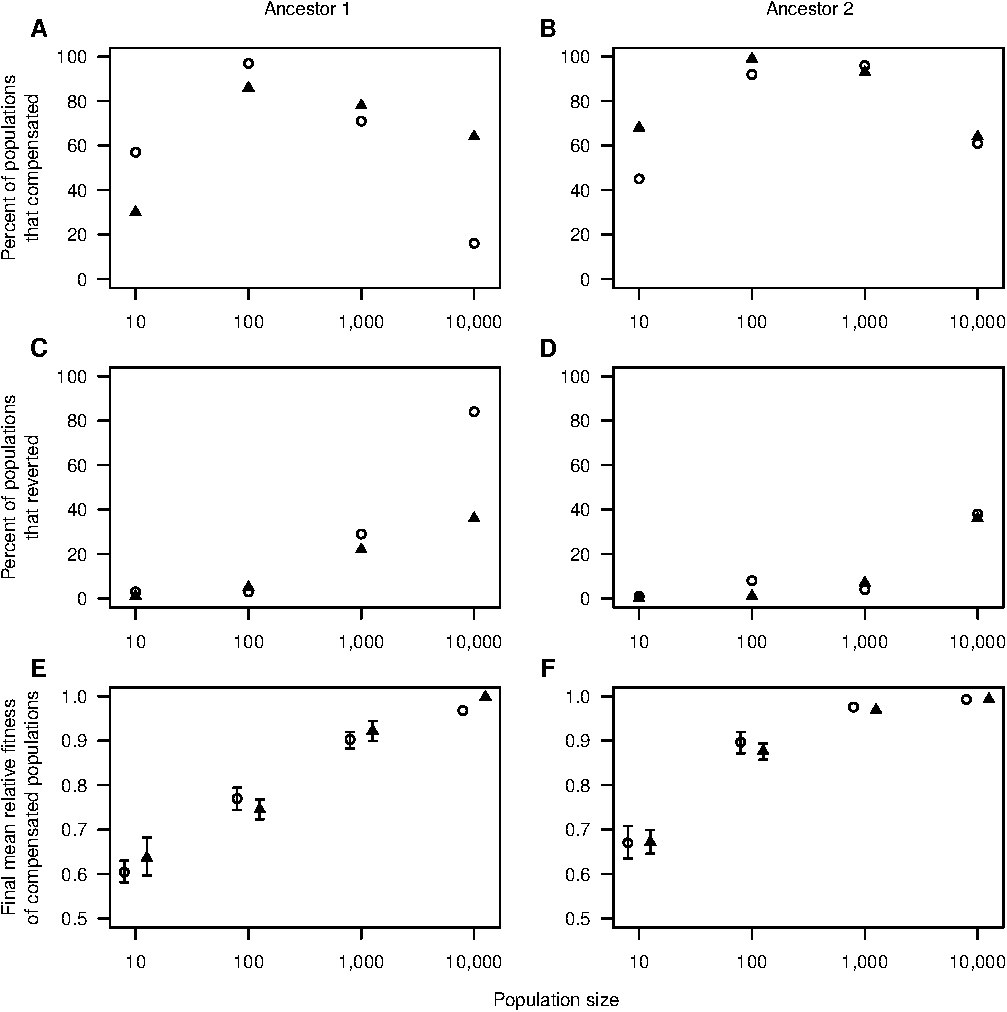
\includegraphics[width=\linewidth]{effect-N.pdf}
\end{center}
\caption{{\bf Effect of population size on compensation.}
  %
  (A) The proportion of runs that underwent compensatory evolution
  for ancestor 1 and (B) ancestor 2.
  %
  (C) The proportion of runs that reverted
  for ancestor 1 and (D) ancestor 2.
  %
  (E) The proportional increase in fitness for compensatory runs
  for ancestor 1 and (F) ancestor 2.
  %
  Open circles ($\ocircle$) represent the first mutant replicate
  while solid triangles ($\blacktriangle$)
  represent the second mutant replicate.}
\label{fig:N_comp}
\end{figure}



The reason that the probability of compensatory adaptation
at population sizes of 10,000 was lower than that at 100 or 1,000
was that the probability of reversion
at population sizes of 10,000 was higher than that at 100 or 1,000.
%
However, this did not explain the reason that the probability of compensation
at population size of 10 was lower than that at 100 or 1,000
because reversion at population size of 10 was very unlikely.
%
I observed that at population size 10
many populations decreased in fitness or did not change in fitness.
%
The number of populations that decreased in fitness
for each mutant was 27, 45, 36, and 27.
%
The number of those whose fitness stayed the same (within 1\%) was
13, 24, 19, and 9 (listed in the same order as above).
%
In contrast, for population size of 100, only 1 of them
decreased in fitness out of all 400 runs, and 8 of them stayed the same.
%
Therefore, many of the populations at size 10 that did not compensate
were accumulating deleterious mutations due to the small population size.



\subsection{Effect of mutation rate}

I evolved the four mutants with relative fitness of 0.5
under five mutation rates each: 0.0001, 0.001, 0.01, 0.1, and 1.0
(mutations per genome per generation).
%
Each of these 16 experiments was replicated 100 times,
starting with 1,000 genetically-identical individuals,
and evolved for 10,000 updates ($\sim$~850 generations).
%
The population size was kept at 1,000 throughout each experiment.
%
I found that when the mutation rate was $>$~0.0001,
the probability of compensatory adaptation
was high across the mutation rates I tested
(Figures~\ref{fig:U_comp}A and \ref{fig:U_comp}B),
except for the second mutant based on the first ancestor
(Figure~\ref{fig:U_comp}A, triangle at mutation rate 0.001),
in which 69\% of the time the population's fitness did not increase.
%
When the mutation rate was 0.0001, the probability of compensation
was low ($\sim$~20\% or less).
%
The probability of reversion increased slightly
the higher the mutation rate for the first ancestor (Figure \ref{fig:U_comp}C),
but it was generally low for the second ancestor (Figure \ref{fig:U_comp}D).
%
The final mean fitness of populations that compensated
was generally higher the higher the mutation rate,
but for the second ancestor the final fitness was lower
at a 1.0 mutation rate than that at 0.1
(Figures \ref{fig:U_comp}E and \ref{fig:U_comp}F).



\begin{figure}
\begin{center}
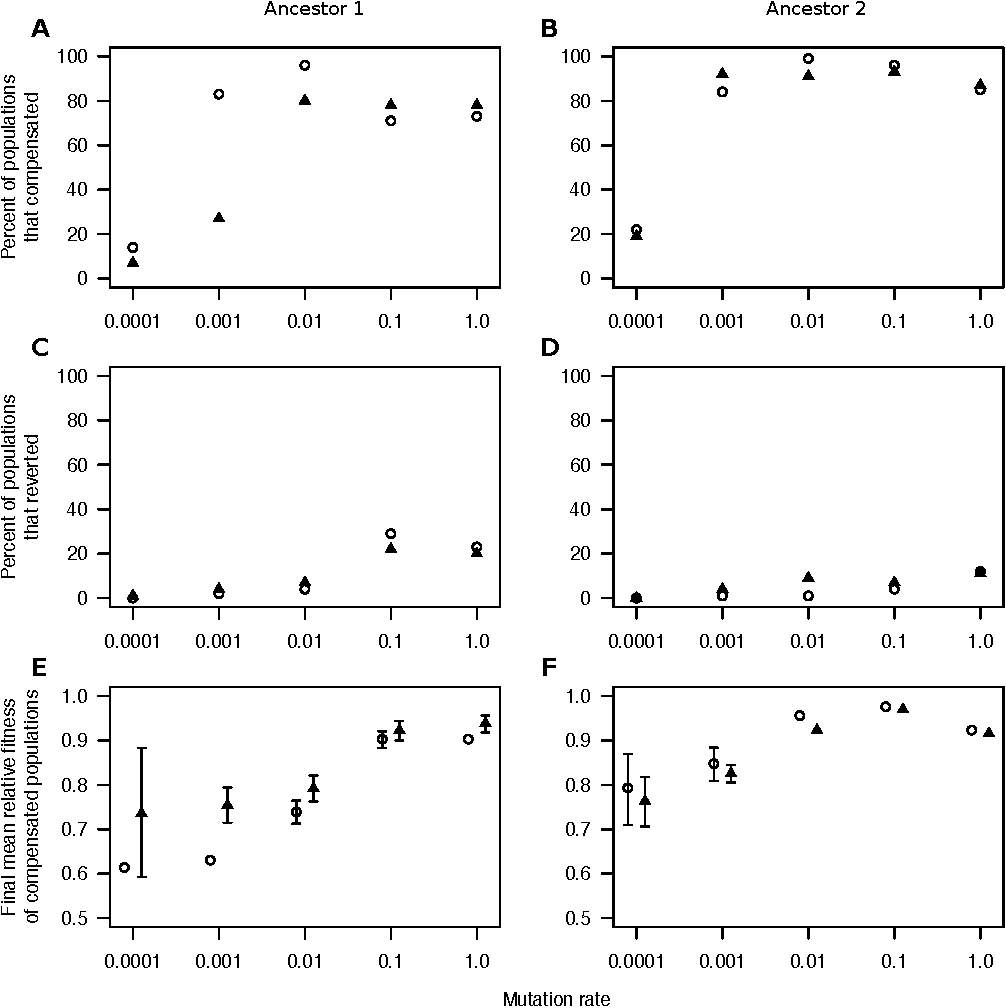
\includegraphics[width=\linewidth]{effect-U.pdf}
\end{center}
\caption{
  {\bf Effect of mutation rate on compensation, reversion,
  and final population fitness.}
  %
  Open circles ($\ocircle$) and dashed lines
  represent the first mutant replicate
  while solid triangles ($\blacktriangle$) and solid lines
  represent the second mutant replicate.
  %
  Error bars are bootstrap 95\% confidence intervals of the mean.}
\label{fig:U_comp}
\end{figure}



In the analysis of population size, reversion was highest
at the highest population size (10,000) because
the total number of mutations that arose was highest,
maximizing the likelihood that a revertant mutation appeared.
%
At the highest mutation rate (1.0),
the total number of mutations that arose was the same
as those in which the population size was 10,000
(10,000~individuals~$\times$~0.1~= 1,000~= 1,000~individuals~$\times$~1.0).
%
However, I found that reversion was less likely at a mutation rate of 1.0
(compare Figure \ref{fig:N_comp}C at population size 10,000
with Figure \ref{fig:U_comp}E at mutation rate 1.0).
%
The reason may be that at the higher mutation rate,
in which all types of mutations have a greater chance of arising,
the revertant mutation often arises on organisms with other mutations,
therefore introducing the possibility of negative epistasis.
%
To test this, I performed a similar analysis as in the initial mutation
fitness, where I calculated the number of generations in which a reversion
stopped being beneficial in populations that did not eventually revert.
%
The expectation is that the sooner reversions stop being beneficial
the stronger that negative epistasis is with other mutations.
%
I found that reversion stopped being beneficial sooner
at higher mutation rate than at lower mutation rate
(Figure~\ref{fig:first-update-rev-bad-U}),
indicating that negative epistasis was strongest at higher mutation rate.



\begin{figure}
\begin{center}
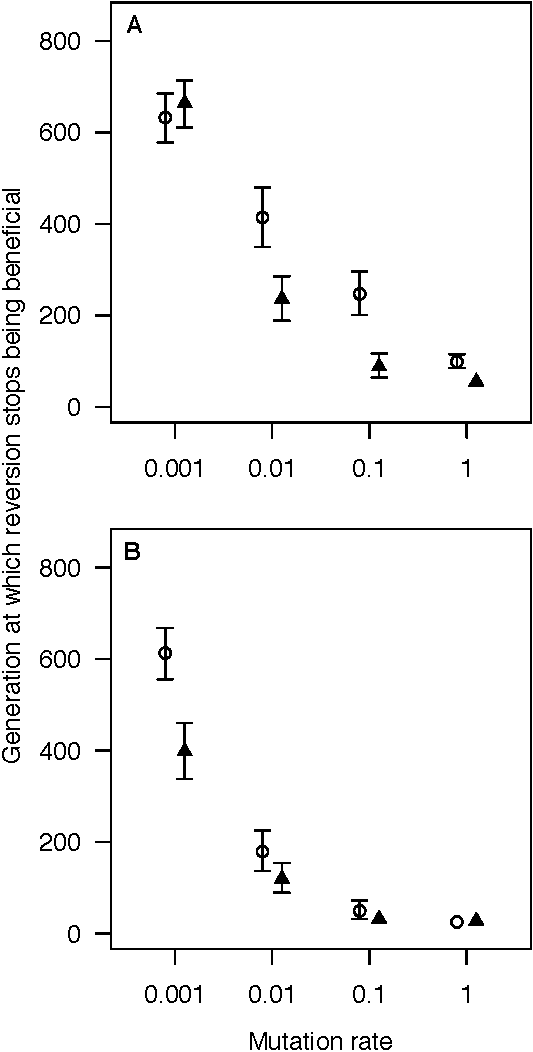
\includegraphics[width=3.5in]{first-update-rev-bad-U.pdf}
\end{center}
\caption{
  {\bf Generation at which reversion stopped being beneficial
  at various mutation rates.}
  %
  (A)~Ancestor~1 and (B)~Ancestor~2.
  %
  Open circles ($\ocircle$) and dashed lines
  represent the first mutant replicate
  while solid triangles ($\blacktriangle$) and solid lines
  represent the second mutant replicate.
  %
  Error bars are bootstrap 95\% confidence intervals of the mean.}
\label{fig:first-update-rev-bad-U}
\end{figure}



\section{Discussion}

Our results corroborate previous findings that compensatory adaptation
is a common alternative to reversion \citep{bur99,moo00,lev00,mai02,est11}.
%
\citet{lev00} stated that ``compensatory evolution
establishes an adaptive valley that is difficult to traverse and thus return to
the ancestral genotype \ldots'' and identified two reasons for this:
(1) there are more compensatory mutations than a revertant mutation and
(2) in serial transfers, population bottlenecks hinder the spread of reversions.
%
They found in their experiments that both processes were going on: ``the rate
of compensatory mutation exceeds that of reversion by at least a factor of 10''
and 2/8 experiments reverted using a higher bottleneck but 0/12 experiments
reverted using a smaller bottleneck.
%
In my populations, there is no serial passage (like a chemostat), so I do
not have the problem of bottlenecks, although populations are limited in size.
%
Yet I see a lot of compensation, meaning that bottleneck
reason is not as important as other factors.
%
Instead, I found that negative epistasis between compensatory mutations
and a revertant (i.e., absence of the deleterious mutation)
prevented the revertant from spreading in a population.



\subsection{Availability of compensatory mutations}

\citet{moo00} and \citet{san05}
found that low-fitness mutants compensated faster than high-fitness mutants.
%
The reason was that, as \citet{moo00} explained,
a compensatory mutation in a low-fitness mutant
has a higher selective coefficient than in a high-fitness mutant
(assuming the compensatory mutation increases fitness relative to the mutant
equally for low-fitness and high-fitness mutants).
%
An alternative explanation,
which \citet{moo00} also discussed
but lacked the evidence to support it,
was that there may be more compensatory mutations available
in low-fitness mutants than in high-fitness mutants.
%
In fact, this was exactly what I found
in the digital mutants (Figure~\ref{fig:comp_avail}).
%
Our results support \citet{whi03},
who said ``when something is broken it is easier to improve than
when in is fully functional'' and \citet{poo05b},
who found a positive relationship between the negative effect
of a deleterious mutation and the probability of compensation.
%
The reason for this that \citet{poo05b} concluded was that
``deleterious mutations with large effects
on fitness may tend to affect a broader range of phenotypic components.
Severely deleterious mutations would therefore generate a larger
mutational target for compensatory interactions.''
%
This must be going on in my populations because the more severe
the deleterious mutation, the more tasks that are being knocked out.
%
I did not find, as \citet{san05} found,
that low-fitness mutants improved in fitness more than high-fit mutants
(Figures~\ref{fig:W_comp}E and \ref{fig:W_comp}F).



\subsection{Effect of initial mutant fitness}

Compensatory mutations depend upon the original deleterious mutation
they compensate, such that they may be deleterious when the deleterious mutation
is removed, such as when reversion occurs \citep{sch97,poo05,lev00}.
%
Negative epistasis between compensatory mutations and revertant mutations
prevented reversion from being beneficial earlier for low-fitness mutants
than for high-fitness mutants (Figure~\ref{fig:first-update-rev-bad-W}).
%
Reversion in low-fitness mutants may have stopped being beneficial earlier
than high-fitness mutants for two reasons.
%
The first reason may be that because in low-fitness mutants
there are many more compensatory mutations available
than in high-fitness mutants (Figure~\ref{fig:comp_avail}),
more mutations fix in low-fitness mutants \citep{moo00,san05}, so that
when a reversion appears, it does so in the genetic background
with many mutations, in which there are more chances for negative epistasis.
%
The second reason may be due to the fact that large-effect
compensatory mutations, which are more likely to fix in low-fitness mutants
cause large-effect negative epistasis.
%
I clearly see the latter reason going on: large-effect compensatory mutations
have stronger negative epistasis with the revertant mutation.
%
I cannot, however, exclude the former, and it is likely going on as well.
%
The importance of all this is that as compensatory adaptation proceeds,
it becomes increasingly harder for reversion to occur,
and populations are obligated to diverge in unique evolutionary paths
because typically there are multiple ways to compensate \citep{pau07}.
%
This decreasing probability of reversion as compensatory adaptation proceeds
has been inferred in mammalian evolution \citep{soy12}.



\subsection{Population size}

Previous studies have generally found that reversion is more common
in large populations \citep{bur99,arg07}.
%
\citet{bur99} found that in two of their large populations
(1,000 and 10,000) a single step recovered fitness substantially.
%
The single step for population 1,000 recovered fitness completely
and it may have been a revertant mutation, although this is unknown.
%
Smaller populations recovered fitness stepwise, and therefore
could not have been revertant mutations,
and their smallest populations increased in fitness very slowly.
%
Our results corroborate their findings and
those of \citet{san05} in that
the probability of reversion increased with population size
and the fitness of populations was greater the greater the population size.
%
In contrast, \citet{mai02} observed that
compensation happened more readily at greater population size
(even in the millions), and reversion was hardly observed.
%
The difference may have been due to differences in mutation rate:
viruses and my digital organisms have high mutation rates
that may have caused revertants to appear more frequently.
%
Both \citet{bur99} and \citet{mai02}
found that fitness was highest when the population size was highest,
as I did (Figures~\ref{fig:N_comp}E and \ref{fig:N_comp}F).
%
However, \citet{est03} argued that no reversion occurred in their
study at their population size of about 10,000, possibly because their mutation
rate was very low ($4.4 \times 10^{-8}$ per nucleotide per generation).



As \citet{poo00} found, compensatory mutations sometimes helped ``freeze''
the mutational meltdown that could have occurred in small populations.
%
But there is a limit in population size in which even compensatory adaptation
cannot save because of the overwhelming effects of drift \citep{poo05}.
%
I found that at population size of 10, many populations decreased in fitness
as they accumulated deleterious mutations.
%
Even severely deleterious populations can be compensated, and do so quickly,
but little can be done about small populations.



\subsection{Mutation rate}

\citet{mai02} found that the rate
of compensatory adaptation in \emph{Salmonella typhimurium}
was higher in a mutator strain (i.e., higher mutation rate).
%
\citet{per10} arrived at a similar result
using a mutator strain of \emph{Pseudomonas aeruginosa}.
%
Our results corroborate this trend, except at very high mutation rates,
where the probability of reversion increased and thus compensation decreased
(Figure~\ref{fig:U_comp}).
%
However, I found that the rate of reversion was not as high as expected
(based on my treatments with population size)
because the window of opportunity for reversion to be be beneficial
was very small at high mutation rates (Figure~\ref{fig:first-update-rev-bad-U}).
%
The reason was that at high mutation rates,
the revertant mutation is likely appear on a genetic background
with other mutations that could cause negative epistasis.



\subsection{Conclusions}



The fixation of compensatory mutations,
which alleviate the negative effects of fixed deleterious mutations,
is a common process in which populations recover from deleterious mutations.
%
Reversion is an alternative process,
but the competing process of compensation
dictates the window of opportunity for which reversion could happen.
%
Populations with large-effect deleterious mutations
have the most number and largest of compensatory mutations available.
%
In addition, large-effect compensatory mutations
have strong negative epistasis with the revertant mutation,
causing a smaller window of opportunity for reversion
the lower the fitness of the population.
%
Larger populations increase the probability of reversion
because there are greater chances for reversion to appear
within its widow of opportunity.
%
However, although a greater mutation rate has a similar effect,
it also shrinks reversion's window of opportunity
because other mutations are also likely to be present,
thereby causing negative epistasis.
%
Small populations and low mutation rate slow down adaptation
in general, so both compensation and reversion are less likely to occur,
but very small populations are likely to decline in fitness.



\section{Materials and Methods}



\subsection{Evolution of ancestors}

Starting with a digital organism with a genome length of 200,
I derived 20 asexual ancestral populations.
%
This initial organism could reproduce but could not perform any tasks.
%
I set the grid (or `world') size to 10,000 individuals
and the point mutation rate to 0.1 per genome per generation.
%
Populations were evolved in the default nine-task environment,
re-configured to add the bonus for each task performed,
rather than multiply its power of two.
%
I allowed 20 replicate asexual populations
to evolve for 500,000 updates ($\sim$~40,000 generations).
%
I then chose two asexual populations
whose consensus sequence could perform all nine tasks.
%
The consensus sequences of these two populations
served as the ancestral genotypes from which mutants were derived.


\subsection{Construction and evolution of mutants}

From each ancestor, I generated every possible single mutant (5,000)
and chose five pairs of mutants,
each pair with the following relative fitnesses:
0.1, 0.3, 0.5, 0.7, and 0.9 ($\pm$~0.025).
%
I ensured that the only allele at the mutant locus
that could fully recover fitness was the ancestral, revertant, allele.
%
If I could not find mutants with the above conditions for any ancestor,
I chose another ancestral genotype that could perform all nine tasks
and repeated the method for generating mutants.
%
In total, I obtained 20 mutants: 10 for each of the two asexual ancestors.


\subsection{Detection of compensatory adaptation}

To determine whether a population compensated or recovered,
I looked at the consensus sequences at the end of 10,000 updates
($\sim$~850 generations).
%
If the fitness of the consensus sequence reached 99\% of the
ancestral sequence and the allele at the mutant position
changed (to either the ancestral or to something else),
then the population was said to have reverted.
%
The reason I also considered non-ancestral alleles as reversions
is that substitutions at the mutant locus could represent
neutral alleles in the original ancestor;
this ``effective reversion'' is common in some viruses \citep{arg07}.
%
If the fitness of the consensus sequence was higher than the
mutant sequence and the allele was not the ancestral allele,
then the population was said to have compensated
(so both full and partial compensation were clumped together).
%
I included substitutions as compensations when the recovery
was partial for similar reasons as above: the mutant allele
likely has neutral mutations that are effectively equivalent.



\subsection{Estimation of the expected time for reversion}

I estimated the expected time (in updates) at which a new reversion
destined to fixation appeared.
%
To do this, I went through each update $t =$ 100, 200, \ldots, 10,000
(my data's resolution) and stopped at update $t$ with probability $p(t)$,
the probability that a new reversion appears between updates $t - 100$ and $t$
and is destined to fixation.
%
I calculated $p(t)$ as $A_{100} f(s(t))(1 - p(t - 100))$, where $A_{100}$
is the probability that a reversion appears within 100 updates,
and $f(s(t))$ is the probability that a new reversion with
selection coefficient $s(t)$ is destined to fixation (methods explained below).
%
The $1 - p(t - 100)$ is the probability that a reversion destined to fixation
did not appear in the previous update.
%
This process was repeated 100 times for each replicate run
in the treatment testing the effect of the initial fitness
(except for replicates that actually reverted because that would
interfere with calculating a reversion's selection coefficient).
%
I estimated the expected time for two different cases:
(1) the revertant's relative fitness is always 1.0 (i.e., without epistasis)
and (2) the revertant's relative fitness depends on the genetic background
on which it appears (i.e., with epistasis).



For either case, the probability $A_{100}$ that a reversion appears
within 100 updates will be the same,
but the probability of fixation $f(s(t))$ will be different because
$s(t)$ depends on whether there is epistasis.
%
To estimate $A_{100}$, I ran 100 Avida experiments where the configuration was
identical to the default experiment (except that the initial population
consisted of organisms that could not perform any tasks).
% Will readers know what the "default" experiment is?
%
During the experiments, every time a specific mutation appeared
(e.g., the position and allele of a reversion for one of my treatments),
I recorded the update at which this happened.
%
(Because the mutation rate was the same for all runs in the treatment
that tested the initial fitness, the choice of revertant to record
does not matter because the probability that any specific mutation appears
is the same for all mutations.)
%
I then binned each recorded update into bins of size 100,
counted the number in each bin, and divided that number by 100
(because there were 100 replicate runs).
%
I found that the mean of $A_{100}$ was 0.1915
with a standard deviation of 0.0443.



As mentioned before, the probability of fixation $f(s(t))$
depends on whether there is epistasis because $s(t)$ depends on this.
%
However, given a specific value of $s(t)$, call it $s$,
I can estimate its fixation probability.
%
To do this, I created every possible mutant of the first ancestor
and calculated their fitness, which gave us various values of $s$
for a revertant (calculated as $1 - w(m) / w(a)$,
where $w(m) / w(a)$ is the relative fitness of the mutant).
%
I discarded any mutants with either zero fitness
or a fitness greater than the ancestor's,
as these would result in an $s$ value less than or equal to 0
(not a beneficial reversion).
%
Then, for each unique value of $s$, I populated a new Avida world of 1,000
identical mutants and a single revertant (i.e., the ancestor).
%
(Because several different mutants sometimes had the same $s$,
I picked the first such mutant in the above configuration.)
%
I let each population run in replicates of 100 for 10,000 updates
($\sim$~850 generations) and zero mutation rate.
%
After removing one outlier, which had 1.0 fixation probability,
I fit two line segments to the data such that together they minimized
the sum of the squared residuals (the first line was anchored
at 0.001 fixation probability for $s$ of 0).
%
I found that when $s < 0.28$, $f(s) = 1.813s$
(with residual standard deviation 0.09584) and when $s \ge 0.28$,
$f(s) = 0.2414s + 0.4382$ (with residual standard deviation of 0.0643).



I estimated the revertant's selection coefficient $s(t)$
as $\overline{w}_{R}(t) - \overline{w}(t)$,
where $\overline{w}_{R}(t)$ is the revertant's mean relative fitness
and $\overline{w}(t)$ is the population's mean relative fitness
between updates $t$ and $t - 100$.
%
Because I recorded data at updates 0, 100, 200, \ldots, 10,000,
I estimated $\overline{w}_{R}(t)$ and $\overline{w}(t)$
as the mean value between those at $t$ and $t - 100$.
%
In the case where there is no epistasis, $\overline{w}_{R}(t)$ was always 1.0.
%
In the case where there is epistasis,
$\overline{w}_{R}(t)$ was the mean relative fitness of the population
where each individual in the population was given the revertant mutation.
%
These analyses were conducted for each replicate run
in which reversion did not happen (total of 1,643 runs).



\section{Acknowledgments}

This material is based in part upon work supported by
the National Science Foundation under Cooperative Agreement No. DBI-0939454.
%
Any opinions, findings, and conclusions or recommendations
expressed in this material are those of the author(s)
and do not necessarily reflect the views of the National Science Foundation.



\end{doublespace}

\begin{lit_cited}
\end{lit_cited}
\addcontentsline{toc}{section}{LITERATURE CITED}

% Temporarily remove section number from bibliography title
\renewcommand\bibsection{\center\section*{\bibname}}

\bibliographystyle{apalike}
\bibliography{comp_rate}

\renewcommand\bibsection{\section{\bibname}}

\begin{doublespace}

\hyphenation{a-mong post-zy-got-ic wheth-er ac-cu-mu-lat-ed}

\chapter{Compensatory adaptation causes rapid incipient speciation}
\label{chap:comp_spp}

\section{Introduction}

Biological speciation is the evolution of reproductive isolating
barriers that prevent populations from interbreeding \citep{coy04}.
%
One potentially important barrier causes `intrinsic postzygotic isolation,'
in which hybrids are sterile or inviable from developmental, physiological,
or behavioral abnormalities \citep{coy04}.
%
Intrinsic postzygotic isolation is believed to commonly evolve
from genetic incompatibilities: negative epistatic interactions
among population-specific alleles inherited by the hybrids \citep{pre10}.
%
Alleles in a population may arise and spread by natural selection,
but the selective pressures involved are often unknown \citep{sch09}.
%
In order to infer the selective pressures that ultimately caused
population-specific alleles involved in genetic incompatibilities,
studies using methods in genetic mapping and molecular genetics
have helped identify `speciation genes' and their functions
\citep{noo06,mah11}.
%
Many of these genes involve the internal environment of the cell,
such as cellular housekeeping, genetic regulation, genetic conflict,
and coevolution between nuclear and mitochondrial genomes \citep{noo06,wol10}.
%
Interestingly, these genes often appear to have been driven
by natural selection \citep{noo06}, suggesting that adaptation to the internal,
genetic environment (as opposed to the external, ecological environment)
can lead to intrinsic postzygotic isolation \citep{pha09,pre10}.



One class of adaptation to the genetic environment
is compensatory adaptation, in which secondary mutations
compensate for the effects of accumulated deleterious mutations
\citep{har96,bur99,moo00,lev00,mai02,est03,est11}.
%
Deleterious mutations may accumulate in a population
through genetic drift \citep{lan94,lyn95},
hitchhiking with beneficial mutations \citep{chu11},
transient environmental changes \citep{bjo00},
or spread of selfish genetic elements \citep{pre10}.
%
Compensatory adaptation recovers and maintains the original phenotype
via stabilizing selection (i.e., selection against extreme phenotypes),
and thus leads to genotypic, not phenotypic, changes \citep{har96}.
%
Populations undergoing independent compensatory adaptation
will therefore diverge genetically, accumulating their own unique set
of deleterious and compensatory mutations.
%
Hybrids between such compensated populations would acquire
a mismatched set of deleterious and compensatory mutations,
exposing genetic incompatibilities that reduce hybrid fitness
\citep{har96,orr01,kon02,kul04,lan07,sch09b,pre10},
%
In this way, compensatory adaptation may lead to
intrinsic postzygotic isolation.



However, whether compensatory adaptation can lead to postzygotic isolation
remains to be tested experimentally.
%
Here I perform such an experiment to answer the following questions:
(1)~does postzygotic isolation evolve from independent compensatory adaptation?
(2)~what is the strength of genetic incompatibilities formed?
and (3)~what is the relative contribution of compensatory mutations
and deleterious mutations to postzygotic isolation?
%
Answering these questions requires that I identify
both deleterious and compensatory alleles,
which involves genetic manipulations that test the allelic
effects of each type of mutation.
%
For example, compensatory mutations must not be beneficial
in the absence of the deleterious mutations they compensate,
and thus they must be tested on their own.
%
Such genetic manipulations, however, are difficult even in
model systems, where genetic tools have been greatly advanced.



Therefore, I conducted my experiments using the artificial life system
Avida \citep{ofr04} (see p. \pageref{sec:avida}),
which has been used previously to study various questions
in evolution \citep{len99,len03,cho04,mis06,ele07,ele08,mis10}.
%
Avida has enabled research on evolving genetic systems
that would have been difficult in natural systems \citep{ada06},
and the similarities between digital and biological organisms
in many evolutionary phenomena have been remarkable \citep{wil02,ada06}.
%
Avida enhances the benefits of microbial systems
(i.e., short generation times, considerable replication,
easy manipulation and storage of genomes),
while being a true instance of evolution of a genetic system,
where the generality of evolutionary principles can be tested
\citep{len99,ele08,mis06}.
%
Specific to this study, Avida allowed us to easily insert deleterious mutations
of various effect sizes, carry out thousands of hybridizations,
and individually identify compensatory mutations.



Using Avida, I isolated mutants with deleterious mutations
from a well-adapted ancestor, and I allowed those mutants to evolve
in replicate for thousands of generations.
%
I then hybridized compensated populations and measured their fitness
to test for postzygotic isolation,
and I identified individual compensatory mutations to determine
their strength and contribution to postzygotic isolation.
%
I found that (1) postzygotic isolation occurred between compensated populations,
(2) the strength of incompatibility among compensatory mutations
was greater than among neutral mutations, and
(3) compensatory mutations contributed as much as deleterious mutation
to postzygotic isolation.
%
Our results suggest that compensatory adaptation may be an important
mechanism by which genetic incompatibilities and
thus intrinsic postzygotic isolation evolve.
%
Because I used a non-specific genetic system to test this hypothesis,
my results can be generalizable to biological organisms and motivate
future tests in biological organisms.



\section{Results}

Starting with a sexually-reproducing, haploid digital organism
that was not adapted to its environment but could replicate,
I allowed three independent populations to evolve
for about 250,000 generations.
%
I used the most common genotype of each adapted population
as an independent ancestor for all subsequent experiments.
%
From the ancestors, I isolated 472 mutants
with 1-5 random irreversible mutations
whose combined negative fitness effect was either
small ($\Delta W$~=~0.01-0.1) or large ($\Delta W$~=~0.1-0.9).
%
As a control, I also isolated 74 neutral mutants ($\Delta W$~=~0.0)
with the same range of mutations per genome as those
in the small-effect and large-effect treatments (Table~\ref{tbl1}).
%
I then allowed populations founded by each mutant (including the controls)
to evolve for about 6,000 generations
in identical environmental conditions as their ancestor.
%
I regarded a population as compensated if its most common genotype
(1)~had a fitness at least equal to that that of its ancestor,
(2)~did not acquire mutations that were beneficial on their own, and
(3)~did not acquire mutations that were deleterious when they first appeared.



\begin{table}
\centering
\begin{tabular}{lccc}
Treatment & Ancestor & Mutants & Compensated \\
\hline
        & 1 & 25 & - \\
Neutral & 2 & 25 & - \\
        & 3 & 24 & - \\
\hline
        & 1 & 71  & 10 \\
Small   & 2 & 199 & 15 \\
        & 3 & 69  & 6  \\
\hline
        & 1 & 44  & 9 \\
Large   & 2 & 44  & 5 \\
        & 3 & 45  & 6 \\
\hline
\end{tabular}
\caption{Number of mutants and compensated populations per ancestor for
  the different treatments}
\label{tbl1}
\end{table}



\subsection{Reproductive isolation via compensation is rapid}

In nature, subpopulations that split off from their ancestral population may
come into secondary contact with their ancestor or with another subpopulation.
%
To model these two scenarios, I performed two types of hybridizations:
(1)~between compensated populations and their ancestor (`AC')
and (2)~between pairs of compensated populations (`CC').
%
I also performed these two types of hybridization on the control populations
(i.e., those that evolved starting with neutral mutations).
%
Note that these hybridizations were performed after all experimental evolution
had completed, i.e., populations evolved independently.
%
I found that the mean fitness of hybrids for both hybridization types
was lower than that of hybrids from control populations
(in Fig.~\ref{fig1}, compare `Control' hybrids with `Del.~+~Comp.' hybrids).
%
Surprisingly, whether populations compensated for
small- or large-effect deleterious mutations
did not have a significant effect on mean hybrid fitness
(in Fig.~\ref{fig1}, the 95\% bootstrap confidence intervals overlap for
`Small-effect Del.~+~Comp.' and `Large-effect Del.~+~Comp.').
%
These findings show that intrinsic postzygotic isolation developed faster
during compensatory adaptation than during neutral evolution,
regardless of the fitness effect size of the initial deleterious mutations.



\begin{figure}
\centering
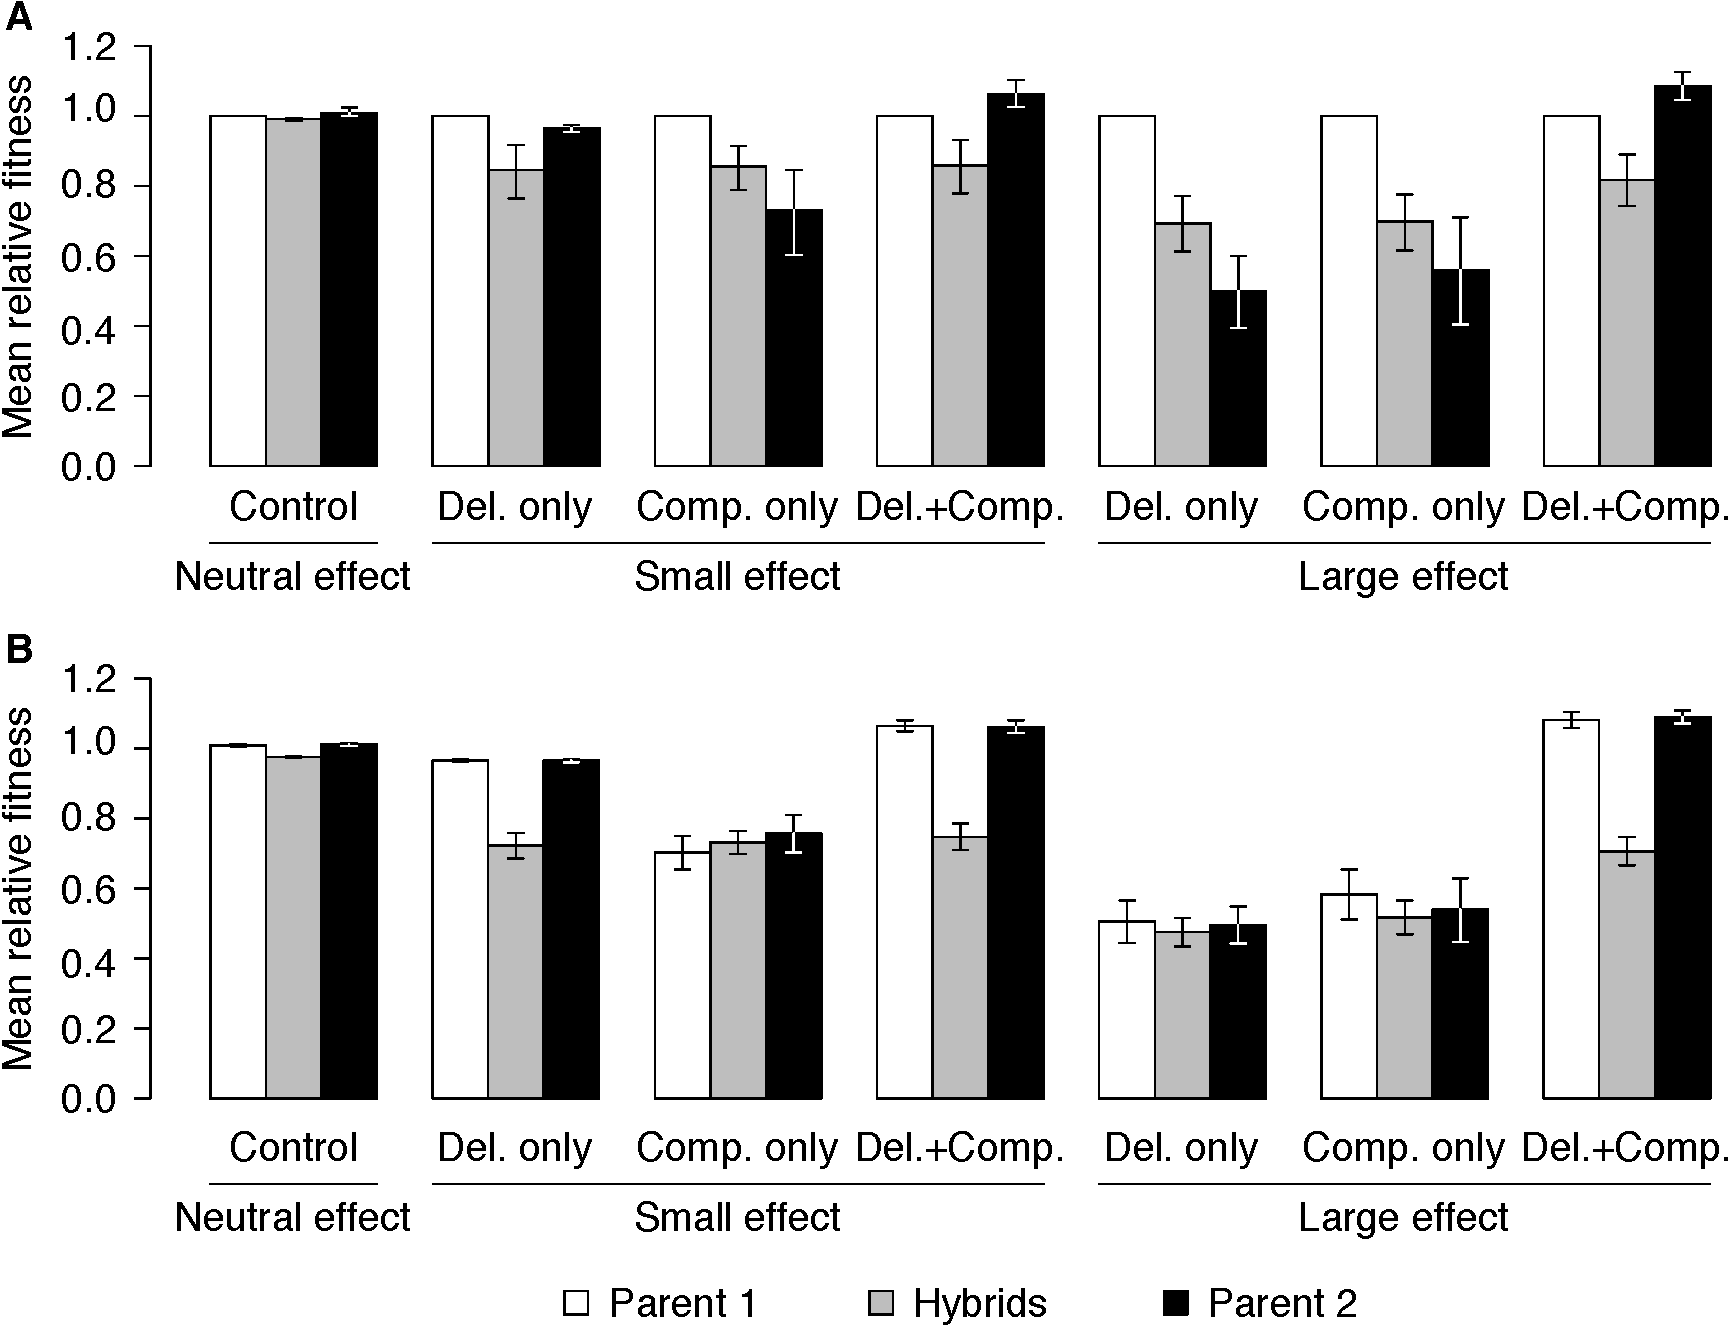
\includegraphics[width=\linewidth]{fig1.pdf}
\caption{Fitness of hybrids after 25,000 updates of parental evolution.
  Populations compensated for either small-effect or large-effect
  deleterious mutations.
  (A) Hybridizations between compensated genotypes and their ancestor.
  (B) Hybridizations between pairs of compensated genotypes
  sharing the same ancestor.
  `Del. Alone' include only the initial deleterious mutations
  before compensation,
  `Comp. Alone' include only the compensatory mutations after compensation,
  and `Del. + Comp.' include both deleterious and compensatory mutations.
  `Control' include all mutations accumulated neutrally.
  Error bars are 95\% bootstrap confidence intervals.}
\label{fig1}
\end{figure}



\subsection{Compensatory adaptation forms strong genetic incompatibilities}

Compensated populations acquired 2-10 mutations at the end of the runs,
while control populations acquired only 0-1 mutations.
%
Compensated populations thus had greater potential for creating
a greater number of genetic incompatibilities than control populations.
%
To determine whether compensated populations created stronger
genetic incompatibilities than control populations,
I accounted for the number of mutations acquired by each type of population.
%
If hybrids between compensated genotypes
have stronger genetic incompatibilities
than hybrids between control genotypes,
then the rate at which hybrid fitness decays
with the number of inherited mutations
should be greater for hybrids between compensated genotypes
than for hybrids between control genotypes.
%
In other words, the slope of the line relating
the number of mutations in hybrids
with the hybrid fitness should be greater
for hybrids between compensated genotypes
than for hybrids between control genotypes.



Before I performed this test, however,
I generated a new set of 250 control genotypes
because my experimental control populations
acquired only 0-1 mutations after about 6,000 generations.
%
To generate the new control genotypes,
I introduced 2-10 neutral mutations into ancestral genotypes,
which was within the range of number of mutations in compensated genotypes.
%
I then fit a least squares linear relationship between
the mean number of mutations in hybrids
and the hybrid fitness for each treatment
(i.e., neutral-, small-, and large-effect for both AC and CC hybrids).
%
I found that the slope of this linear relationship
was significantly greater for hybrids between compensated genotypes
than for hybrids between control genotypes (Fig.~\ref{fig2}B),
but was not significantly greater for AC hybrids (Fig.~\ref{fig2}A).
%
Our findings suggest that genetic incompatibilities
involving deleterious and compensatory mutations in hybrids
were stronger than those among neutral mutations.



\begin{figure}
\centering
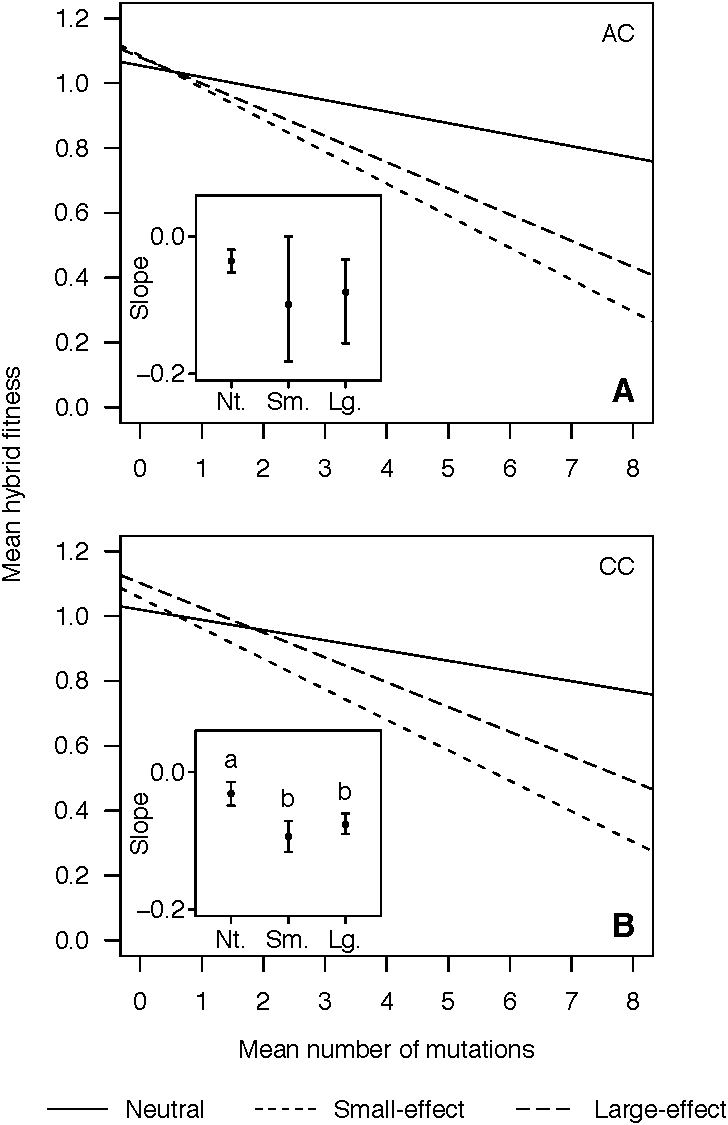
\includegraphics[width=\linewidth]{fig2.pdf}
\caption{Strength of genetic incompatibilities in hybrids.
  (A) Least squares linear fit of the mean number of mutations in hybrids
  between ancestor and compensated genotypes (AC) against their mean fitness.
  (B) Same as (A) except for hybrids between pairs of compensated genotypes
  (CC). Insets: Means and 95\% bootstrap confidence intervals of each slope
  where shared letters indicate overlapping confidence intervals.}
\label{fig2}
\end{figure}



\subsection{Both deleterious and compensatory mutations
  contribute to reproductive isolation}

Although I have shown that genetic interactions
involving deleterious and compensatory mutations
may form strong genetic incompatibilities rapidly,
I have yet to quantify the relative contributions
of each type of mutation to the formation of genetic incompatibilities.
%
At first glance, Fig.~\ref{fig1}
may suggest that compensatory mutations
contributed little to reproductive isolation
because hybrids between genotypes before compensation (`Del.~only')
had fitnesses as low as hybrids after compensation (`Del.~+~Comp.').
%
However, hybrids between compensated genotypes in which deleterious mutations
were reverted to the ancestral state also had low fitnesses
(in Fig.~\ref{fig1}, compare `Comp.~only' hybrids to `Del.~+~Comp.' hybrids),
suggesting that compensatory mutations
also contributed to postzygotic isolation.



To establish more directly the extent to which incomplete sets
of deleterious and their corresponding compensatory mutations
contributed to postzygotic isolation,
I generated genotypes with different proportions
of deleterious and compensatory mutations.
%
I generated such genotypes by creating every possible hybrid
between a compensated genotype and its ancestor.
%
For each genotype, I then measured its fitness and calculated
the proportion of deleterious and compensatory mutations
relative to the compensated parental genotype.
%
I performed this analysis on all compensated genotypes
for both the small-effect and large-effect treatments.
%
I found that, unless genotypes contained either
all or none of their parent's deleterious and compensatory mutations,
their fitness was low (Fig.~\ref{fig3}),
suggesting that both deleterious and compensatory mutations
contributed to postzygotic reproductive isolation.



\begin{figure}
\centering
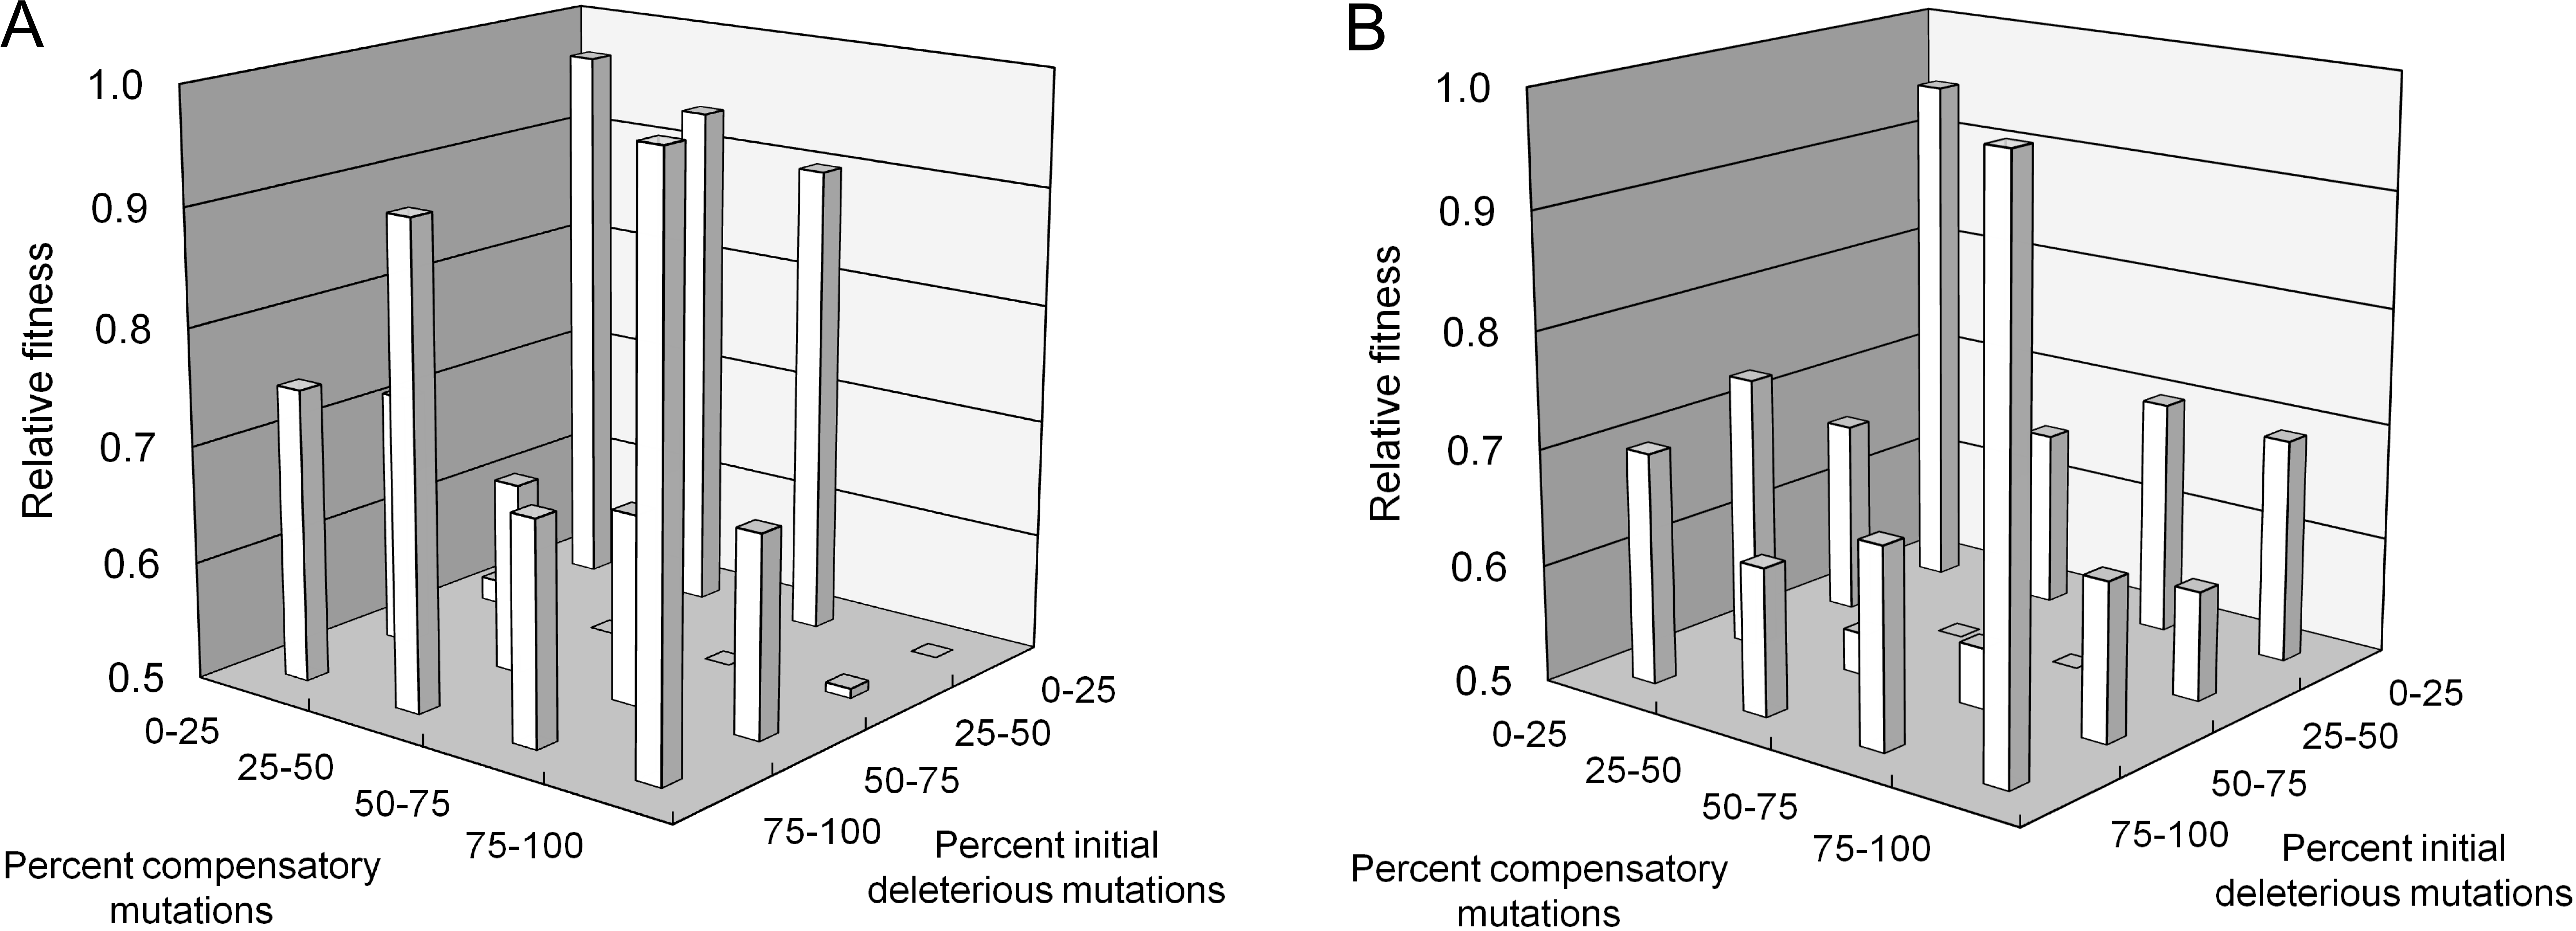
\includegraphics[width=\linewidth]{fig3.png}
\caption{Fitness of hybrids with intermediate parental contributions
  of deleterious and compensatory mutations.
  (A) Mean fitness of hybrids between the ancestor
  and compensated parents that inherit the specified percent of small-effect
  deleterious and compensatory mutations. (B) Same as (A) except for
  large-effect deleterious mutations.}
\label{fig3}
\end{figure}



\section{Discussion}

Most genes involved in intrinsic postzygotic isolation,
i.e., hybrid sterility or inviability
due to developmental or physiological abnormalities,
show strong signatures of positive selection \citep{pre10}.
%
Surprisingly, many of these genes
are not adaptations to the external, ecological environment
but to an impaired internal, genetic environment
(see Table~\ref{tbl1} in \citep{pre10}).
%
An example of adaptation to an impaired genetic environment
is adaptive compensation of deleterious mutations
\citep{har96,bur99,moo00,lev00,mai02,est03,est11}.
%
Populations undergoing independent compensatory adaptation
will diverge genetically
and may form genetic incompatibilities,
causing intrinsic postzygotic isolation
\citep{orr01,kon02,kul04,coy04,lan07,sch09b,pre10}.
%
Under this scenario, I asked:
how rapidly does postzygotic isolation evolve?
what is the strength of genetic incompatibilities?
and what are the relative contributions
of compensatory and deleterious mutations to isolation?



Using an artificial life system,
I found that postzygotic isolation
due to compensation was rapid:
hybrids between compensated populations
had significantly lower fitness
than hybrids between populations that did not undergo compensation,
regardless of the effect size
of the initial deleterious mutations.
%
I also found that compensatory adaptation
formed stronger genetic incompatibilities:
the rate at which hybrid fitness
decayed with the number of mutations
was significantly greater
for hybrids between compensated populations.
%
Finally, I found that both
deleterious and compensatory mutations
contributed to postzygotic isolation:
hybrids with different proportions
of compensatory and deleterious mutations
were unfit unless all or none
of both types of mutations were present.



Two important implications to the genetics of postzygotic isolation
can be drawn from my findings.
%
First, evidence of genotypic diversification between species
may not correlate with phenotypic diversification.
%
This is because compensatory adaptation can build up genetic differences
without altering phenotypic characteristics.
%
In fact, compensatory adaptation may act under stabilizing selection
to maintain phenotypes despite continual accumulation of
deleterious mutations \citep{har96}.
%
Second, evidence of positive selection
at loci that contribute to speciation (`speciation genes')
may not always be the result of diversification
due to ecological adaptation
but instead be the footprint of compensatory adaptation.
%
Our results corroborate the view that
adaptation to the internal, genetic environment
may be important in the development
of intrinsic postzygotic isolation \citep{pre10,pha09}.



In describing his mechanism of founder speciation, Ernst Mayr stated that
``\dots\ the mere change of the genetic environment may change the
selective value of a gene very considerably'' \citep{tem08}.
%
In cases where founder events cause the fixation or high frequency
of deleterious mutations, compensatory adaptation may provide a
mechanism by which genes with altered selective values change
in allele frequency.
%
Furthermore, Templeton's model of genetic transilience recognizes
that founder populations may be affected by genetic drift
while new mutations and recombination increase genetic variation \citep{tem08}.
%
Genetic drift alone can raise the frequency of deleterious mutations
in a founder population while increased genetic variation
may introduce new compensatory mutations on which selection can act.
%
Our study using experimental evolution with populations of digital organisms
suggests that such compensatory mutations can rapidly generate
postzygotic barriers, and therefore supports a novel genetic mechanism
for models of founder or peripatric speciation.
% Check out paper:
% Increased mitochondrial mutation frequency after an island colonization: positive selection or accumulation of slightly deleterious mutations?


Our study took advantage
of the recent implementation of sexual reproduction
in the artificial life platform Avida \citep{mis06},
and extended its application
as proof of principle to the field of speciation.
%
I demonstrated that Avida is a useful tool to complement
other approaches in speciation research as it allows for
the direct observation of evolution and reproductive isolation in action.
%
Furthermore, my conclusions will motivate additional research
into compensatory adaptation as a viable mechanism for speciation,
to be further explored in biological systems.
%
The notion that organisms construct or choose
their own microhabitats \citep{lew00}
suggests that organisms are somewhat
resilient to changes in the external environment.
%
This reduced emphasis on the external environment in evolution
is supported by my conclusion that environmental differences
between allopatric populations are not essential for genetic diversification.



\section{Materials and Methods}

\subsection{Strains and experimental conditions}

The starting digital organism I used was the `default' sexually-reproducing
organism in Avida, with a genome length fixed to 80 instructions.
%
The population size was set to 10,000 organisms,
and the copy mutation probability was set to 0.0005 per instruction
(i.e., 0.04 per genome per generation).
%
Other types of mutations, such as insertions or duplications,
were not permitted because they may disrupt homologous recombination.
%
Digital organisms were configured to reproduce sexually,
and the two recombinant offspring were set to replace random individuals
in the population when no free space was available.
%
The `diverse' environment rewarded the nine tasks
commonly used in Avida experiments \citep{len03}.
%
The small genome size of digital organisms caused reversions
to be common during compensatory adaptation in preliminary runs.
%
To guarantee that genotypic changes were due to mutations at secondary loci%
---as has been observed in biological organisms \citep{bur99,est11}---%
I prevented reversions from occurring.



\subsection{Isolation of mutants}

To generate mutants for the small-effect and large-effect treatments,
I first generated sets of 10,000 random mutant genotypes
for each evolved ancestor until either four mutants
with the desired number of mutations and effect size were found,
or until 100 million mutants had been searched.
%
For the small-effect treatment, effect sizes of
0.01, 0.02, 0.03, 0.04, 0.05, 0.06, 0.07, 0.08, 0.09, and 0.1
(each with up to a 0.0049 deviation) were identified for genotypes carrying
1, 2, 3, 4, or 5 mutations.
%
For the large-effect treatment, mutants with effect sizes of
0.1, 0.2, 0.3, 0.4, 0.5, 0.6, 0.8, and 0.9 (with up to a 0.049 deviation)
for each mutation number of 1, 2, 3, 4, and 5 were identified.
%
(Effect size is the difference between
the fitnesses of the ancestral and the mutated genotype,
relative to the ancestral genotype.)
%
I isolated a total of 339 small-effect mutants
(after running the above procedure twice) and 133 large-effect mutants.
%
I implemented a different searching procedure for neutral mutations
because the probability of several random mutations resulting
in a neutral genotype was very low.
%
To find neutral mutants, I first generated 10,000 single-mutants
and selected the first one that was neutral
(i.e., relative fitness of exactly 1.0).
%
This procedure was repeated starting with the neutral mutant until
the desired number of mutations was reached or until the
recursion was exhausted.
%
I isolated a total of 74 neutral mutants.



\subsection{Compensated populations}

I regarded a population as compensated if its most common genotype
(1)~reached a fitness of at least 1.0 relative to its ancestor,
(2)~did not acquire mutations that were beneficial on their own, and
(3)~did not acquire mutations that were deleterious when they first appeared.
%
To determine condition (1), the most common genotype at the end of a run
was isolated and its fitness relative to its ancestor was measured.
%
If its relative fitness was equal to or greater than 1.0,
then the population was considered compensated.
%
To determine condition (2), the fitness effect of each
secondary mutation in the most common genotype of the population
was tested in the genetic background of the ancestor.
%
If any `transformant' had a relative fitness above 1.0,
then that population was not considered as compensated
because mutations were beneficial on their own
(i.e., generally beneficial, not compensatory);
otherwise, the population was considered compensated.
%
To determine condition (3), I sequentially examined the
most common genotype of the population about every three generations.
%
If the gain of any mutation resulted in a lower fitness than the
genotype at the previous third generation,
then that population was not considered as compensated;
otherwise, the population was considered compensated.



\subsection{Hybridization method}

Hybrids were created by the same method in which Avida
creates recombinants during sexual reproduction:
the genetic region between two crossover points
were exchanged between two parents to produce two offspring.
%
Hybridizations, whether between compensated populations
and their ancestor or between pairs of compensated populations,
involved creating every possible hybrid
between the most common genotypes of each population.



\subsection{Statistics}

To compare the fitness of hybrids among treatments (Fig.~\ref{fig1}),
I determined whether their 95\% bootstrap confidence intervals overlapped.
%
For each treatment, bootstrap replicates were set to contain the
same number of samples per ancestor---established as the mean number
of observed samples per ancestor---in order to minimize any
potential bias from the fact that ancestors yielded different
numbers of compensated populations.
%
All bootstraps contained 10,000 replicates.
%
To determine the linear relationship between the number of mutations
in hybrids and their fitness (Fig.~\ref{fig2}),
I fit a linear least squares model to each bootstrap replicate.
%
I compared the 95\% bootstrap confidence intervals of the slopes
among treatments to establish the relative effect of mutation number
on hybrid fitness.
%
Statistical analyses were performed in R (ver.~2.8.1).



\section{Acknowledgments}

I thank R. E. Lenski, D. W. Schemske, and C. Ofria, I. Dworkin,
and A. Gerstein for helpful discussion and comments on the manuscripts.
%
This work was supported by the Quantitative
Biology Initiative at Michigan State University (MSU)
and the BEACON Center for the Study of Evolution in Action.
%
Computational experiments were made possible by the
High Performance Computing Center at MSU.
%
This material is based in part upon work supported
by the National Science Foundation under Cooperative Agreement No. DBI-0939454.
Any opinions, findings, and conclusions or recommendations
expressed in this material are those of the authors
and do not necessarily reflect the views of the National Science Foundation.

\end{doublespace}

\bibliographystyle{apalike}
\bibliography{comp_spp}

\begin{doublespace}

\chapter{Ecological and mutation-order speciation in digital organisms}
\label{chap:ecol_mo}



\section{Introduction}

Reproductive isolation between populations
often evolves as a byproduct of independent adaptation
to new environments \citep{coy04,sch09,sob10}.
%
When these environments' selective pressures are different,
divergent selection can cause populations
to acquire different, often incompatible, alleles.
%
This divergent process can generate reproductive isolation
both in nature \citep[reviewed in][]{run05,sch09}
and in laboratory experiments \citetext{\citealp{det07,det08};
reviewed in \citealp{ric93} and \citealp{fry09}}.
%
Complete reproductive isolation due to this process
is known as `ecological speciation' \citep{sch09}.
%
On the other hand, if the environments' selective pressures
are similar or identical (parallel or uniform selection),
populations may diverge genetically
by the chance fixation of different alleles.
%
Although laboratory experiments and theoretical studies suggest that
such process may lead to `mutation-order speciation' \citep{sch09,nos11},
its effectiveness in generating reproductive isolation
compared to ecological speciation is unknown.



The main purpose of this study is to directly compare
the strength of reproductive isolation
generated by ecological and mutation-order processes.
%
Specifically, we measure both the degree of postzygotic isolation
(i.e., hybrid inviability)
as well as the amount of genetic divergence between populations
evolved under either different environments or the same environments.
%
Because there is a higher chance of parallel evolution
when environments are similar \citep{sch09b},
we expect that postzygotic isolation and genetic divergence
under a mutation-order process will be weaker than under an ecological process.



We also examine the effect of migration
on both ecological and mutation-order processes.
%
Migration between populations increases the chance of gene flow,
which often slows genetic (and thus adaptive) divergence,
although gene flow can also promote divergence \citep{gar06,ras08}.
%
We vary the amount of migration between populations
under both ecological and mutation-order processes,
from allopatry to sympatry.
%
We expect that migration will have a stronger negative effect
on the evolution of reproductive isolation under mutation-order scenarios
because, under uniform selection, an adaptive mutation
that arises in one population is also selectively
favored in the other \citep{sch09,nos09b,nos11}.



We also examine how the environments' dimensionality
(i.e., number of selective pressures)
affects the strength of reproductive isolation
for both ecological and mutation-order processes.
%
In high-dimensional environments,
there are more opportunities for populations
to adapt in different ways \citep{ric93,nos09},
which may lead to stronger reproductive isolation
for both ecological and mutation-order processes.
%
High dimensionality, however, may also constrain speciation
when trade-offs among adaptive traits hinder adaptation
and therefore decrease the probability of reproductive isolation.



Finally, we examine one possible cause for differences
in hybrid fitness between ecological and mutation-order processes.
%
As populations adapt to their local environments independently,
there is no guarantee that alleles acquired in one population
will interact positively, or even neutrally, in the hybrid
with alleles acquired in the other population \citep{coy04}.
%
Negative interactions between alleles from two populations
are known as Dob\-zhan\-sky-Mul\-ler incompatibilities (DMIs),
and both ecological and mutation-order process
may cause them to form and thus lead to postzygotic isolation \citep{sch09}.
%
It is unknown, however, whether ecological or mutation-order speciation
differ in their propensity to produce DMIs.
%
Although a mutation-order process may be expected to have
fewer DMIs initially than an ecological process
because uniform selection selects for the same alleles,
such expectation diminishes the more populations diverge \citep{sch09}.



In this study, we use the software Avida to carry out our experiments.
%
Avida \citep{ofr04} is an artificial life research platform
where digital organisms evolve due to genetic variation, inheritance,
and differential reproduction (see Methods).
%
Avida has been used previously
in a wide range of ecological and evolutionary studies
\citep[e.g.,][]{len03,cho04,ele07,ost07,mis10}.
%
There are several reasons for using digital organisms to study evolution:
we can observe millions of generations in a few days,
conduct hundreds of replicate experiments,
easily manipulate genomes,
and accurately measure fitness.
%
Digital organisms in Avida are not meant to specifically mimic
the details of real biological organisms.
%
Instead, digital organisms have a unique genetic system (see Methods).
%
Despite these differences, the general principles
that make evolution possible are still the same,
which allows Avida to be used to test the generality
of evolutionary theories and hypotheses.
%
Indeed, several evolutionary properties
have been found to be remarkably similar to that of biological organisms
\citep{wil02,ada06}
(e.g., the distribution of mutational effects, the types of epistasis,
and the genetic architecture of sexual organisms).
%
Digital organisms improve on simple two-locus models of speciation
because in Avida, traits are complex,
involving multiple loci and epistatic interactions among alleles \citep{len99}.



\section{Methods}

\subsection{Avida}

Experiments with digital organisms were carried out using Avida (ver.~2.9.0),
freely available at \url{http://avida.devosoft.org}.
%
In this section, we provide a brief overview of Avida;
for a full description, see \citet{ofr04}.
%
Avida is highly configurable, so unless otherwise noted,
the following description applies to the default settings.
%
In Avida, each digital organism consists of several components:
a linear sequence of instructions (akin to a haploid genome),
memory space in the form of registers and stacks,
pointers to memory locations,
and a central processing unit (CPU) that executes instructions.
%
The instruction set makes up an assembly-like programming language,
consisting of instructions for arithmetic operations,
memory manipulation (e.g., swap registers or push into a stack),
conditional execution (i.e., `if' statements), iteration (looping),
input/output operations, and allocation and copying of memory.
%
Organisms execute their instructions sequentially,
sometimes skipping instructions for conditional statements
or repeating the same instructions inside a loop;
when the last instruction is executed,
execution starts again at the first instruction.
%
By executing instructions in their genomes,
organisms are able to (1) replicate and (2) perform computational `tasks'
that affect the speed at which they replicate and thus increase fitness.



To replicate, an allocation instruction creates the memory space
required by the organism's offspring, and a copy instruction inside a loop
allows the organism to copy itself into the new memory space.
%
The copy instruction that allows organisms to replicate
has a configurable probability of making mistakes,
therefore introducing various kinds of mutations
(e.g., point mutations, indel mutations, and slip mutations).
%
By default, replication is asexual.
%
However, Avida may be configured to perform sexual replication,
in which the genomes of two asexually-produced offspring are recombined
by exchanging two randomly-sized regions of their genomes.
%
The offspring (whether clonal or two recombinants) are put into the population
in random locations, replacing whatever organisms were already there.
%
Generations are therefore overlapping, as offspring are born continuously,
replacing older individuals who are likely not their parents.



In addition to replication, genomic instructions allow organisms
to acquire 32-bit input values and use them to perform computational tasks.
%
Tasks are boolean operations, such as NOT, AND, and OR,
and are applied to input values bit by bit.
%
For example, if input values were 8 bits,
the operation 10011101 AND 11101011 would produce 10001001
because 0 AND 0 is 0, 0 AND 1 is 0, 1 AND 0 is 0, and 1 AND 1 is 1.
%
In Avida, however, there is no AND operation nor any other boolean operation
except for NAND, from which all other boolean operations may be built,
a property of NAND known as `functional completeness' in boolean algebra.
%
For example, P AND Q, where P and Q are input values,
is equivalent to (P NAND Q) NAND (P NAND Q),
and P OR Q is equivalent to (P NAND P) NAND (Q NAND Q).
%
Because tasks are made up of the same building blocks (NANDs),
evolved tasks may share the same pieces of code
and therefore may not be completely independent.



When an organism performs a task, the organism's `merit' is increased
by a specific amount, specified in a configuration file, for that task.
%
The merit of an organism is a unitless value used by Avida
to determine the number of instructions an organism may execute each time step.
%
If two organisms had the same merit,
they would execute the same number of instructions at each time step;
however, if one organism had twice the merit as another,
the first organism would execute twice the number of instructions
compared to the second in a single time step.
%
Thus, an organism with twice the merit as another,
would replicate twice as fast.
%
Organisms initially inherit the merit of their parents;
otherwise, new organisms would be at a disadvantage
compared to the rest of the population.
%
The default environment rewards for nine binary (i.e., two-input) tasks,
but the environment can be configured to reward for an additional 68
three-input tasks.



Adaptation in Avida occurs naturally (i.e., it is not simulated),
as a result of the three ingredients required for natural selection:
inheritance, variation, and differential reproduction.
%
Inheritance comes from replication (sexual or asexual),
variation comes from mutation and recombination,
and differential reproduction comes from their rate of replication
(determined by their replication code and performance of tasks).
%
The ability to perform tasks evolves as organisms with the right mutations
replicate faster than others and therefore take over the population.
%
There are many ways in which to perform any one task,
and independently evolved organisms often evolve the same task
in different ways and with different degrees of efficiency.



\subsection{Experimental design}

The Avida configuration files used to run our experiments
are available in the Dryad Data Repository.
%
To generate the ancestral population,
we founded a population with an organism that could replicate
but could not perform any tasks.
%
We then let this population evolve under the default nine-task environment
for 500,000 updates ($\sim$~42,000 generations).
%
An `update' is a measurement of time in Avida, increasing by one each time
organisms execute 60 instructions (on average).
%
For the evolution of the ancestral population,
we set the maximum population size to 10,000 individuals.
%
The length of the genome was set to 200 instructions,
and to ensure homologous recombination
during sexual reproduction, the genome length was fixed.
%
The mutation rate was set to 0.1 mutations per genome per generation.



We then set up four treatments (described below), which we call
`drift,' `ecological,' `mu\-ta\-tion-or\-der 1,' and `mu\-ta\-tion-or\-der 2.'
%
For each treatment,
the population size was set to 2,000 individuals
and divided into two demes, each of size 1,000.
%
In the drift treatment, both demes' environments
were the same as the ancestral (environment `A').
%
For each remaining treatments,
we set up two subtreatments (described below):
low dimensionality and high dimensionality.
%
For this study, dimensionality refers to the number of tasks
for which that environment rewards organisms for performing such tasks.
%
In the ecological treatment, the demes' environments
were different from each other and different from the ancestral
(environments `1L' and `2L' for low dimensionality
and environments `1H' and `2H' for high dimensionality).
%
In the mutation-order 1 treatment,
the demes' environments were the same as each other
but different from the ancestral
(environment `1L' for low dimensionality
and environment `1H' for high dimensionality).
%
Similarly, in the mutation-order 2 treatment,
the demes' environments were the same as each other
but different from the ancestral
(environment `2L' for low dimensionality
and environment `2H' for high dimensionality).



The specific tasks that were rewarded in each environment
remained the same for the rest of this study.
%
The number of tasks for the low and high environments
were chosen as two extremes: two tasks for low dimensionality
and the maximum of 34 (i.e., 68 possible tasks divided randomly
into two demes) for high dimensionality.
%
The specific tasks for environments 1L and 2L were chosen at random
from tasks that were known to evolve within 10,000 updates in preliminary runs.
%
Environments 1L and 2L shared no tasks;
similarly, environments 1H and 2H shared no tasks.
%
The specific tasks rewarded in each environment
are part of the Avida configuration files,
which are available in the Dryad Data Repository.



Each treatment was replicated 20 times
with a different random sample of 2,000 organisms (1,000 per deme)
from the ancestral population.
%
Successive random samples were reused for each treatment,
so that the genotypes in replicate $n$ of a treatment
were the same as the genotypes in replicate $n$ of another treatment.
%
We ran each replicate for 10,000 updates ($\sim$~850 generations).
%
For each run, the entire population of organisms
was saved every 100 updates ($\sim$~8.5 generations).
%
To examine the effect of gene flow,
each replicate was run under eight migration rates
(for the entire length of the run):
0.0 (allopatry), 0.00001, 0.0001, 0.001, 0.01, 0.05, 0.1, and 0.5 (sympatry).
%
Migration rate is the probability of an offspring
being born in a deme different than its parents;
the migrating offspring was placed in a random
location in the other deme (i.e., there were no hybrid zones)
but the parents remained in their own demes.
%
In all, there were 1,120 runs.



We measured the overall strength of selection in each environment
(1L, 2L, 1H, and 2H) at the end of each `ecological' replicate run.
%
First, for every organism in a population that could perform at least one task,
we counted the number of tasks it could perform
and calculated its fitness relative to the mean.
%
We then used linear regression on the relationship between
the number of tasks an organism could perform and its relative fitness.
%
The slope of this line is the strength of selection \citep{con04}.
%
We report these results here, as they are part of the environment
in which populations evolved.
%
For environments 1L and 2L, the mean strengths of selection were
0.3440 (0.3375--0.3562, 95\% bootstrap C.I.) and 0.3353 (0.3341--0.3366),
respectively.
%
For environments 1H and 2H, the mean strengths of selection were
0.2045 (0.1852--0.2248) and 0.1899 (0.1762--0.2041), respectively.
%
We discuss the strength of selection in the Discussion.



\subsection{Postzygotic reproductive isolation}

In this study,
we focus on the evolution of postzygotic reproductive isolation.
%
To measure the strength of postzygotic isolation for each treatment,
we first selected 1,000 random pairs of organisms (one from each deme)
and created one hybrid per pair at the end of each replicate run.
%
We then calculated the fitness of each hybrid
as the mean fitness relative to each parent.
%
Finally, we compared the mean hybrid fitnesses for each treatment---%
the lower this fitness, the stronger the isolation.
%
Note that hybrids were created
after the experiments were finished;
no hybrids were put back into the population.



Two types of hybridizations were performed for creating hybrids
after the populations had evolved.
%
The first followed the method used in Avida for sexual reproduction
(and the way in which all our experimental populations experienced):
a randomly-sized genomic region starting at a random locus was chosen
(both random numbers came from a uniform distribution),
and two recombinant offspring were created by exchanging
the genetic region of one parent with the other (two-point crossover).
%
We randomly chose one of the two offspring as the hybrid.
%
We also performed a more fine-scaled hybridization method,
where each locus of a hybrid had the same probability (0.5)
of it coming from either one or the other parent.
%
This method effectively increased the number of crossover points up to 200
and the number of regions that can be exchanged up to 100.
%
We used this multiple-point crossover method
to break apart coadapted gene complexes,
following the same logic that researchers
use when carrying out parental backcrosses
or intercrosses between hybrids \citep[e.g.,][]{li97,bur99}.
%
Multiple crossover points can expose
incompatible gene complexes between species,
revealing patterns of divergence
that would be difficult to detect with
recombination at only two crossover points.



\subsection{Genetic divergence}



To quantify the homogenizing effects of gene flow,
we calculated the genetic divergence
between each replicate pair of demes
under 0.0 and 0.01 migration for each treatment.
%
Genetic divergence was measured as the fixation index
$F_{\mathrm{ST}} = 1 - H_{\mathrm{S}} / H_{\mathrm{T}}$,
where $H_{\mathrm{S}}$ is the mean heterozygosity of each deme
and $H_{\mathrm{T}}$ is the heterozygosity of both demes
treated as one population \citep[p. 118]{har97}.
%
The heterozygosity of a deme
is the mean heterozygosity at all loci.
%
The heterozygosity at a locus is $H = 1 - \sum_{i = 1}^{n} x_i^{2}$,
where $n$ is the number of alleles segregating at that locus
and $x_i$ is the frequency of the $i$th allele \citep[p. 15]{gil04}.
%
$F_{\mathrm{ST}}$ values between 0 and 0.05
would indicate little or no genetic divergence
between two demes \citep[p. 118]{har97}.
%
We expect that under zero migration
$F_{\mathrm{ST}}$ values will be significantly higher
than those under the 0.01 migration rate.
%
Significance among treatments was determined by comparing their
95\% confidence intervals of the mean $F_{\mathrm{ST}}$.
%
Each confidence interval was estimated by calculating 10,000 means
of random samples (with replacement) of the $F_{\mathrm{ST}}$ values
from the 20 replicates
(i.e., each sample contained 20 $F_{\mathrm{ST}}$ values).
%
The interval between 2.5\% and 97.5\% of means defined the confidence interval.



To test whether gene flow causes the same mutations%
---specifically those involved in performing a task---%
to fix under mutation-order speciation,
we carried out a two-step process to identify and map such mutations.
%
First, to determine whether the fixed mutations in a deme
were necessary to perform a task,
we reverted each locus, one by one, of the deme's consensus sequence
to the ancestral state.
%
If any reversion eliminated the ability to perform a task,
then the allele at that locus must be important for that task.
%
We ignored loci in which a reversion caused
complete inviability of the organism,
as these loci were involved in more than just task performance.
%
Second, we aligned the consensus sequences of each pair of demes
under 0.0 and 0.01 migration and highlighted the mutations we found above.



\subsection{Hybrid phenotypes}

To examine a possible cause for differences
in hybrid fitness between ecological and mutation-order processes,
we counted the number of times that hybrids had low fitness
due to Dob\-zhan\-sky-Mul\-ler incompatibilities (DMIs).
%
Under two-point crossover recombination,
a hybrid is made up of two parental components,
which we call C$_{1}$ and C$_{2}$.
%
If C$_{1}$ or C$_{2}$ contains the instructions to perform a task
but the full hybrid cannot perform that task,
C$_{1}$ and C$_{2}$ must interfere with one another through at least one DMI.
%
To determine whether a hybrid had low fitness due to DMIs,
we constructed two genotypes by making two copies of the hybrid,
where we replaced C$_{2}$ in the first copy, and C$_{1}$ in the second copy,
with the corresponding ancestral genetic region.
%
In this way, we constructed two `component' genotypes,
where each parental component was isolated
in the genetic background of the ancestor.
%
We then determined the tasks that these component genotypes
as well as the original hybrid could perform.
%
If either component genotype could perform a task
but the hybrid could not, then at least one DMI was present
(Figure \ref{fig:hybrid_components}).
%
We performed this analysis on 1,000 hybrids per replicate
in both the ecological and mutation-order treatments
under zero migration, low dimensionality, and two-point crossover recombination.



\begin{figure}
\centering
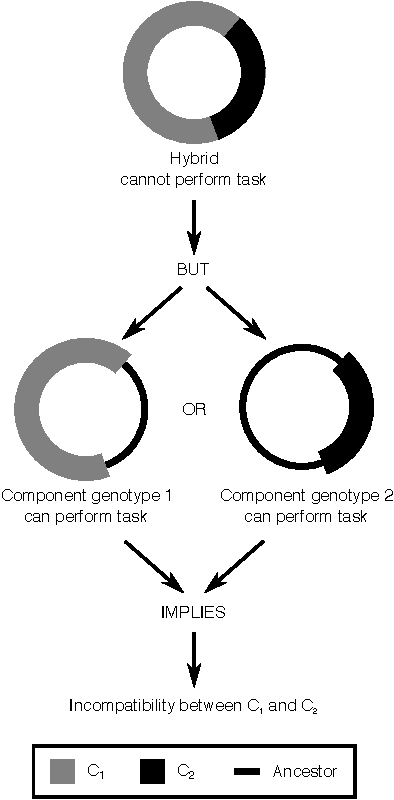
\includegraphics[width=3.5in]{hybrid_components.pdf}
\caption{Method to determine whether a hybrid contains
  genetic incompatibilities.
  %
  A hybrid is composed of two parental components, C$_{1}$ and C$_{2}$.
  %
  Note that a parental component is only the parental region
  inherited by the hybrid; it is not the complete parent.
  %
  If the hybrid cannot perform the task but either parental component can,
  then there must be at least one incompatibility between the components.}
\label{fig:hybrid_components}
\end{figure}



Because in this system an organism's fitness is largely determined
by the number and type of tasks it can perform (i.e., its phenotype),
we identified the tasks that could be performed by each hybrid
for both ecological and mutation-order processes.
%
Note that this analysis is independent of the environment
because an organism may have the ability to perform a task
even if the environment does not reward for it.
%
For simplicity, we focused only on
the zero migration, low dimensionality set of treatments
that were hybridized with a two-point crossover.
%
For the ecological treatment,
hybrids were categorized by the number tasks they could perform:
(`\mbox{0-0}')~no tasks in either environment,
(`\mbox{1-0}')~one task in one environment but none in the other,
(`\mbox{1-1}')~one task in each environment,
(`\mbox{2-0}')~two tasks in one environment but none in the other,
(`\mbox{2-1}')~two tasks in one environment and one in the other,
and (`\mbox{2-2}')~two tasks in both environments.
%
For the mutation-order treatment,
hybrids were categorized by the tasks they could perform:
(`None')~no tasks,
(`1')~task~1,
(`2')~task~2,
and (`1 and 2')~both tasks.
%
For those hybrids that could perform both tasks
in the mutation-order treatment,
we determined the tasks that each hybrid's parental components could perform.
%
We categorized these parental components as
(`0,0')~no parental component performs any task,
(`1,0')~one parental component performs one task but the other none,
(`1,1')~each parental component performs a different task,
and (`2,*')~at least one parental component performs both tasks.
%
This analysis will reveal the reason, at the phenotypic level,
for differences in hybrid performance between ecological
and mutation-order processes.
%
Four replicates from the ecological treatment,
one replicate from the mutation-order 1 treatment,
and six replicates from the mutation-order 2 treatment
were removed from the analysis above.
%
In the ecological treatment, the removed replicates contained parents
that could fortuitously perform a task of the other environment
(even though there was no selective pressure for that task),
and thus it would be unclear from which parent the task was inherited
by the hybrids.
%
In the mutation-order treatments, the removed replicates contained parents
that could not perform both tasks and, therefore, was the reason
that some of the hybrids were unfit.



\section{Results}

\subsection{Postzygotic reproductive isolation}

When hybrids between the evolved demes
were created by recombining a single genetic region (`two-point crossover'),
reproductive isolation between demes
that adapted to different environments (ecological treatment)
was considerably stronger than
reproductive isolation between demes
that adapted to the same environment (mutation-order treatment)
(Figs. \ref{hybrid_fitness}A and \ref{hybrid_fitness}B).
%
With zero migration, for instance,
reproductive isolation in the ecological treatment
was more than twice as strong than in the mutation-order treatment.
%
There was no reproductive isolation between demes
evolving neutrally in the ancestral environment (drift treatment):
the mean hybrid fitness was $>$~0.99 at all migration rates.



\begin{figure}
\centering
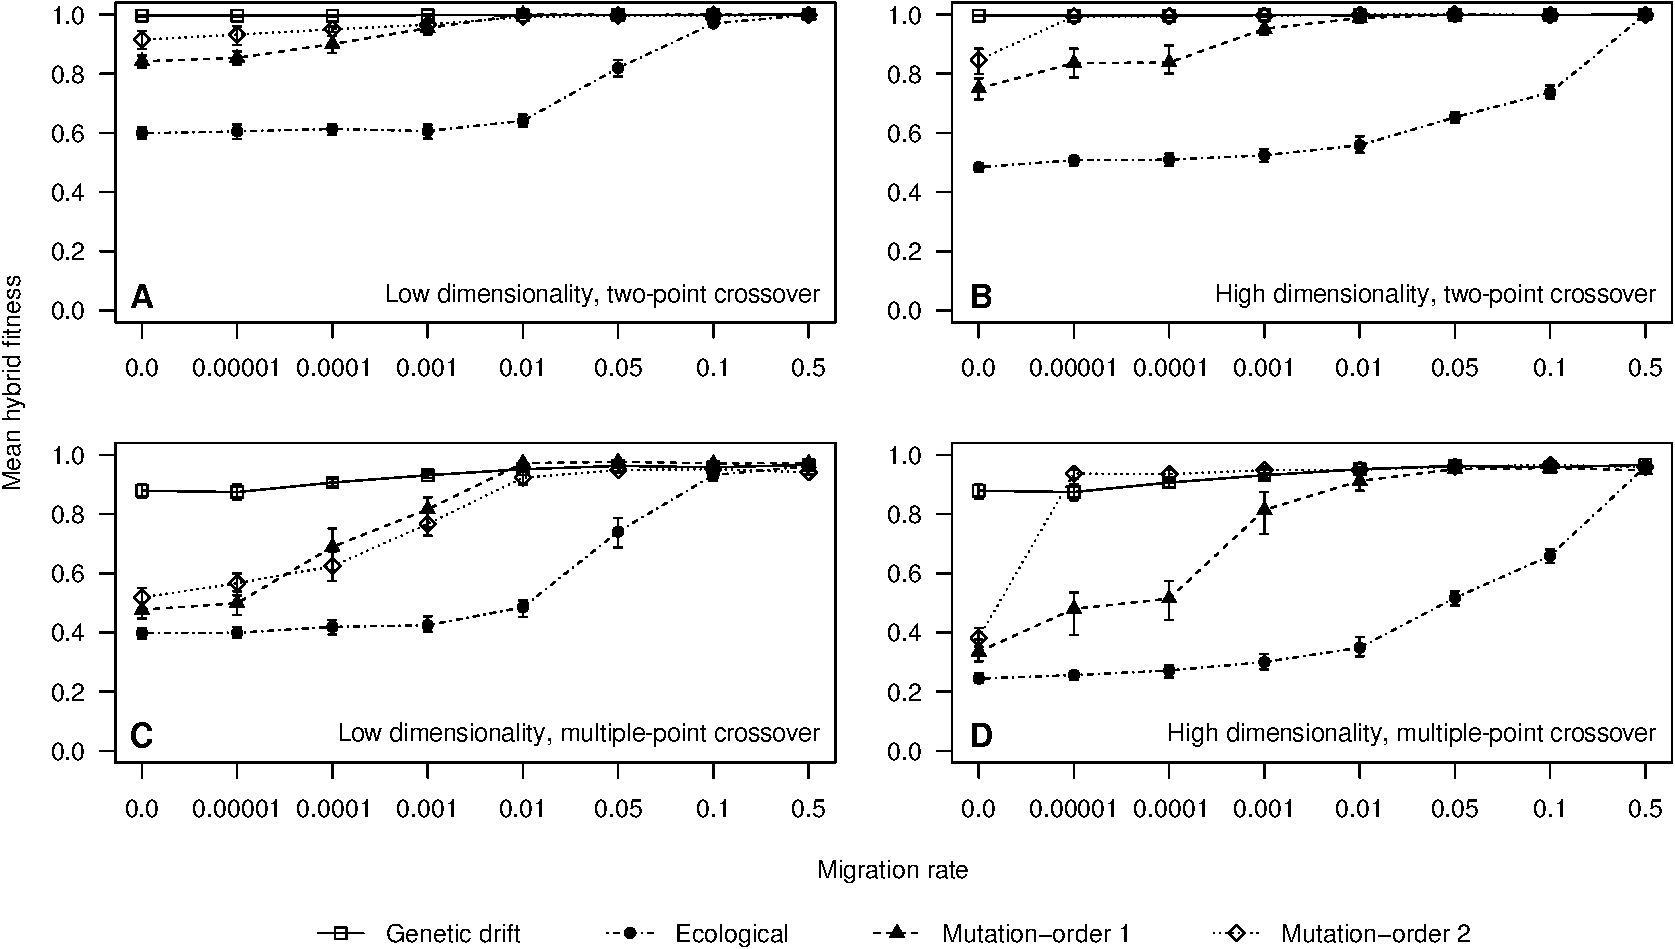
\includegraphics[width=0.95\linewidth]{hybrid_fitness.pdf}
\caption{Mean fitness of hybrids (y-axis)
  between populations evolved under various migration rates (x-axis)
  and different treatments (markers and lines):
  the ancestral environment (`Genetic drift'),
  different new environments (`Ecological'),
  or the same new environment (`Mutation-order 1' and `Mutation-order 2').
  At low dimensionality (A and C),
  the new environments rewarded only two tasks;
  at high dimensionality (B and D),
  the new environments rewarded 34 tasks.
  With two-point crossover (A and B),
  only one region was exchanged when creating hybrids;
  with multiple-point crossover (C and D),
  up to 100 regions were exchanged.}
\label{hybrid_fitness}
\end{figure}



Reproductive isolation in the mutation-order treatment
was more sensitive to gene flow than in the ecological treatment
(Figs. \ref{hybrid_fitness}A and \ref{hybrid_fitness}B).
%
At the 0.01 migration rate, for instance,
the mean hybrid fitness in the mutation-order treatment was $>$~0.98,
but in the ecological treatment reproductive isolation
was almost as strong as without migration.
%
The mutation-order 2 treatment was more sensitive to gene flow
than the mutation-order 1 treatment
(no reproductive isolation at a migration rate of 0.00001).



When the environment rewarded for many tasks (high dimensionality),
reproductive isolation was often stronger than
when the environment rewarded for only two tasks (low dimensionality)
(compare Figs. \ref{hybrid_fitness}A and \ref{hybrid_fitness}B,
Figs. \ref{hybrid_fitness}C and \ref{hybrid_fitness}D).
%
This pattern was most evident in the ecological treatment,
even at moderately high migration rates;
for example, the mean hybrid fitness in the ecological treatment
at 0.1 migration was 0.97 under low dimensionality
but only 0.74 under high dimensionality.
%
In the mutation-order treatments, however,
reproductive isolation under high dimensionality at migration rates $>$ 0
was not always stronger than under low dimensionality,
showing again that mutation-order was sensitive to gene flow.



When hybrids between the evolved demes
were created by recombining up to 100 genetic regions
(`multiple-point crossover'),
reproductive isolation in the ecological and mutation-order treatments
was stronger (Figs. \ref{hybrid_fitness}C and \ref{hybrid_fitness}D).
%
Note that recombination with multiple crossover points was used only
to create hybrids for the calculation of postzygotic isolation;
all populations were evolved under two-point crossover recombination.
%
The mean hybrid fitness with multiple-point crossover
was significantly lower than that with two-point crossover,
dropping 33\% and 48\% in the ecological treatment
for low and high dimensionality (respectively)
and 53\% and 43\% in the mutation-order treatments.
%
The difference in strengths of reproductive isolation
between ecological and mutation-order treatments
was now smaller than that with two-point crossover.
%
Reproductive isolation in the mutation-order treatment
remained more sensitive to gene flow than in the ecological treatment.
%
Reproductive isolation in the genetic drift treatment with little migration
was significantly greater than with two-point crossover.
%
Interestingly, reproductive isolation in the genetic drift treatment
with 0.00001 migration and high dimensionality
was even greater than in the mutation-order 2 treatment.



\subsection{Genetic divergence}

The genetic divergence under zero migration was significantly higher
than that under 0.01 migration for all treatments (Table \ref{tbl_fst}),
demonstrating that gene flow between populations had a homogenizing effect.
%
Under 0.01 migration, the mutation-order treatments had little genetic
divergence ($F_{\mathrm{ST}} <$ 0.05), which was significantly lower than the
ecological treatments, suggesting that the mutation-order treatments were more
sensitive to gene flow than the ecological treatments.
%
Interestingly, the drift treatment under zero migration showed high levels of
genetic divergence, as high as the ecological and mutation-order treatments for
low dimensionality.
%
Under zero migration, the genetic divergence for each treatment for high
dimensionality was significantly higher than those for low dimensionality.
%
Under 0.01 migration, the genetic divergence for the ecological treatment for
high dimensionality was significantly higher than that for low dimensionality,
but for the mutation-order treatments there was no difference in the genetic
divergence between low and high dimensionalities.
%
In agreement with these results,
the sequences for each pair of demes for treatments
under zero migration did not align as well as those
under 0.01 migration (Fig. \ref{task_muts}).
%
These result suggest that the reason that reproductive isolation
was mostly absent under a mutation-order process with gene flow
is that the key mutations that allowed organisms to perform tasks were the same
(i.e., no genetic divergence for task-related mutations).



\begin{table}
\centering
\caption{Genetic divergence ($F_{\mathrm{ST}}$)
  between demes for each treatment.}
\begin{tabular}{llcc}
\cline{3-4}
  & & \multicolumn{2}{c}{Migration rate} \\
\hline
Dimensionality & Treatment & 0.0 & 0.01 \\
\hline
--  & Drift            & 0.3136$^{a}$ & 0.0187$^{b}$ \\
\hline
Low & Ecological       & 0.3173$^{a}$ & 0.1387$^{c}$ \\
Low & Mutation-order 1 & 0.3096$^{a}$ & 0.0186$^{b}$ \\
Low & Mutation-order 2 & 0.3002$^{a}$ & 0.0216$^{b}$ \\
\hline
High & Ecological       & 0.4187$^{d}$ & 0.2680$^{e}$ \\
High & Mutation-order 1 & 0.4221$^{d}$ & 0.0304$^{b}$ \\
High & Mutation-order 2 & 0.3758$^{f}$ & 0.0199$^{b}$ \\
\hline
\multicolumn{4}{p{4in}}{\small\emph{Note:} Shared superscript letters indicate
  that those values are not significantly different
  (95\% bootstrap confidence interval).}
\end{tabular}
\label{tbl_fst}
\end{table}



\begin{figure}
\centering
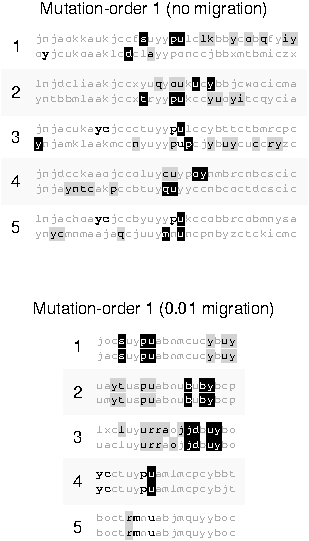
\includegraphics[height=5in]{task-muts.pdf}
\caption{Consensus sequences of the first five evolved replicate pairs of demes
  in the mutation-order~1 treatment under zero migration (top)
  and 0.01 migration (bottom).
  %
  Similar results were observed for the mutation-order~2 treatment.
  %
  Sequences were 200 instructions in length,
  but only the loci that differed among
  each set of five replicates are shown.
  %
  Derived alleles involved in performing a task are highlighted
  (black highlight~=~task~1, gray highlight~=~task~2, bold font~=~both).}
\label{task_muts}
\end{figure}



\subsection{Hybrid phenotypes}

In the ecological treatment,
we found that each replicate had, on average,
268.3 hybrids (218.0--315.8, 95\% bootstrap mean C.I.) of 1,000
that contained at least one DMI between their parental components.
%
In the mutation-order treatments,
this quantity was 77.1 (45.8--111.2) and 128 (83.5--176.5) of 1,000.
%
Therefore, populations that adapted to different environments
accumulated more DMIs than populations that adapted to similar environments.



Because hybrids, on average, inherit half the genome of each parent,
we expected that hybrids, on average, would inherit half the tasks
from each parent (here we focused on the treatments without migration,
low dimensionality, and two-point crossover).
%
In the ecological treatment, we found that hybrids were more likely to perform
zero, one, or two tasks from one parent and none from the other
(Figure \ref{hybrid_counts}A).
%
Less than 10\% of hybrids were able to perform all four tasks.
%
For the mutation-order treatments,
most hybrids could perform both tasks
(Figure \ref{hybrid_counts}B and \ref{hybrid_counts}C),
but because the parents could also perform both tasks,
this information alone did not tell whether hybrids inherited
one task from each parent or some other combination.
%
When we analyzed those hybrids that could perform both tasks,
we found that most inherited both tasks from just one parent
(Figure \ref{fit_hybrid_components}),
although for mutation-order 2
the difference between those
that performed one task from each parent
and those that performed both tasks from one parent
was not significant.
%
Surprisingly, for the mutation-order 1 treatment
there were many hybrids that were fit
even though their parental components
could perform no tasks or just one task
(Figure \ref{fit_hybrid_components}A).



\begin{figure}
\centering
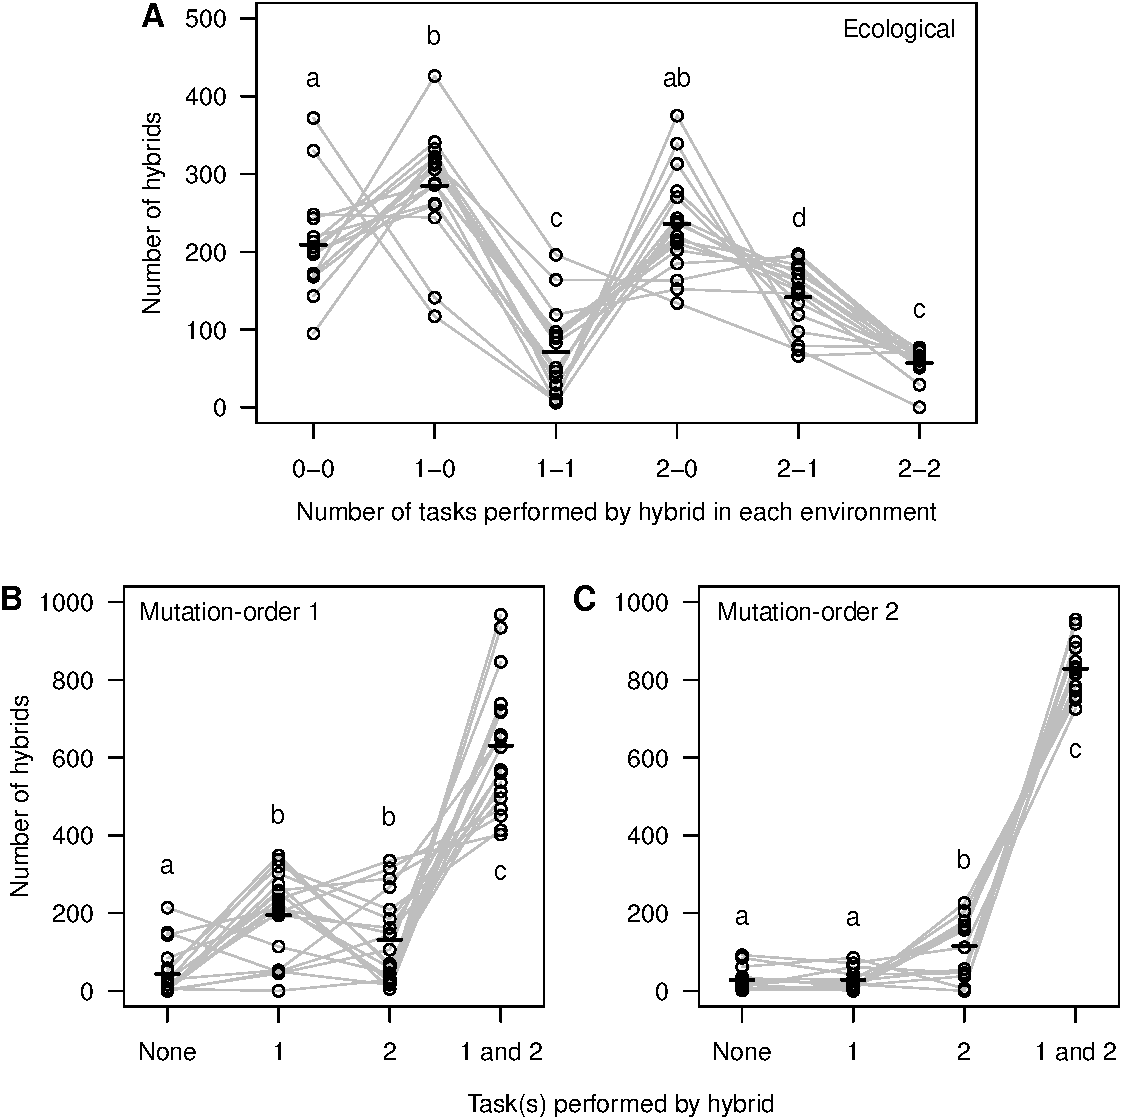
\includegraphics[width=0.95\linewidth]{hybrid_counts.pdf}
\caption{Number of hybrids able to perform certain tasks (see Methods) for
  the (A) ecological, (B) mutation-order-1, and (C) mutation-order-2 treatments
  under zero migration, low dimensionality, and two-point crossover.
  %
  Each point is a hybrid count (out of 1,000) for a single replicate.
  %
  Counts from the same replicate are connected by gray lines.
  %
  The mean hybrid count per category among replicates
  is indicated by a horizontal bar.
  %
  Non-significant differences between the mean hybrid counts
  share the same letter above (or below) the points in each category.}
\label{hybrid_counts}
\end{figure}



\begin{figure}
\centering
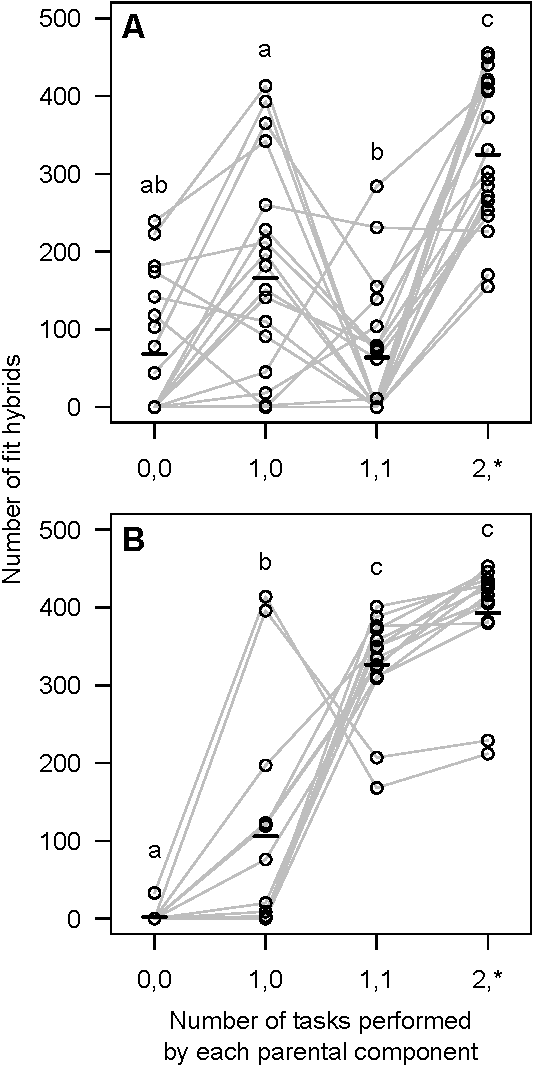
\includegraphics[width=0.95\linewidth]{fit_hybrid_components.pdf}
\caption{Number of fit hybrids (i.e., can perform two tasks)
  whose parental components can perform certain tasks (see Methods)
  for the (A) mutation-order 1 and (B) mutation-order 2 treatments
  under zero migration, low dimensionality, and two-point crossover.
  %
  Each point is a hybrid count for a single replicate.
  %
  Counts from the same replicate are connected by gray lines.
  %
  The mean hybrid count per category among replicates
  is indicated by a horizontal bar.
  %
  Non-significant differences between the mean hybrid counts
  share the same letter above the points in each category.}
\label{fit_hybrid_components}
\end{figure}



\section{Discussion}

In this study, we used experimental evolution of digital organisms
to compare the strength of postzygotic reproductive isolation
generated by ecological and mutation-order processes.
%
We assessed the strength of postzygotic isolation
by measuring the mean hybrid fitness relative to each parent
in its native environment.
%
We found that, using a two-point crossover recombination method,
the mean hybrid fitness was around 55\% under ecological divergence
but around 83\% under a mutation-order process.
%
Other studies have also found that the mean hybrid fitness
is lower under divergent selection than under parallel selection.
%
\citet{det07} found that the mean relative fitness of hybrids
between yeast populations evolved in different environments
(high-salinity and low-glucose) was around 87\%,
but hybrids from populations evolved
under the same environmental conditions were as fit as their parents.
%
Similar patterns were found in a filamentous fungus by \citet{det08},
although in one of the parental environments
hybrids between populations under divergent selection
performed better than hybrids under parallel selection.
%
Along with these studies, our study supports
the view that ecological divergence causes
stronger reproductive isolation than a mutation-order process.



It has been suggested that gene flow during speciation
may be common \citetext{\citealt{coy04}, p. 112; \citealt{nos08}},
which requires that genetic divergence with gene flow be possible.
%
We found that a migration rate of 1\% was not enough to prevent
genetic divergence under an ecological process (Table \ref{tbl_fst}).
%
This finding supports the notion that it is possible for populations
under divergent selection in the face of gene flow to continue to diverge.
%
Under a mutation-order process, however, a migration rate of 1\%
was enough to prevent genetic divergence,
which suggests that mutation-order speciation
is more sensitive to gene flow than ecological speciation.
%
\cite{nos11} also found in their computer simulations
that genetic divergence under a mutation-order process
did not occur $>$~1\% gene flow.
%
One of the mutation-order treatments under high dimensionality
was even sensitive to a migration rate of 0.00001.
%
We speculate that in this treatment (corresponding to environment 2H),
there was one or more large-effect adaptive mutation(s) that,
when migrated to the other deme, spread quickly and homogenized the demes.
%
We conclude that different populations under parallel selective pressures
probably require almost complete isolation for divergence to occur.



Reproductive isolation between populations evolving in high-dimensional
environments has been predicted and observed to be stronger than in single or
low dimensional environments \citep{ric93,nos09,nos09b}.
%
In \emph{Timema} walking-stick insects, for example, reproductive isolation
showed a positive correlation with environmental dimensionality
\citep{nos08b,nos09b}; further examples are reviewed in \citet{nos09}.
%
Most empirical studies, however, rely on incomplete measures of dimensionality
(imagine the difficulty in accounting for all selective pressures in the field).
%
In this study, we were able to control precisely the number of selective
pressures for the low and high dimensionality treatments.
%
We found that under an ecological process, reproductive isolation was stronger
between populations in high-dimensional environments than in low dimensional
environments.
%
Under a mutation-order process, however, this pattern held only when no
migration occurred between populations, but when gene flow was allowed this
pattern went away.
%
Our results support previous findings that dimensionality matters for
ecological speciation but suggests that for mutation-order speciation with gene
flow, environmental dimensionality may not be as important.



This conclusion was also supported by our measurements of genetic divergence:
there was no difference in genetic divergence between low and high
dimensionality for the mutation-order treatments under some gene flow.
%
For the ecological treatment, however, the genetic divergence in high
dimensionality was higher than in low dimensionality and higher than the
mutation-order treatments, again showing that mutation-order treatments were
more sensitive to gene flow.
%
Interestingly, under zero migration the drift treatment (where mutations fixed
neutrally) was as high as the ecological and mutation-order treatments under
low dimensionality, suggesting that most of the divergence in the ecological
and mutation-order treatments was actually the result of neutral fixations and
few adaptive mutations.
%
Indeed, in post-hoc analyses we found that about 90\% of mutational differences
between these treatments were due to neutral fixations, not adaptive mutations.
%
Another result to note is that under zero migration, the ecological and
mutation-order treatments had about the same level of genetic divergence, which
is closer to our result with multiple-point crossover than two-point crossover,
suggesting that in some cases the amount of postzygotic reproductive isolation
and genetic divergence are decoupled.



This decoupling between reproductive isolation and genetic divergence
has been observed in biological populations \citep{ste09,mac12}.
%
In these studies, genetic divergence was not found to be a good predictor
of sexual dimorphism or assortative mating \citep{ste09,mac12}.
%
In some cases, genetically closely related species
were ecologically and phenotypically divergent;
in other cases, genetically distant species
were phenotypically and ecologically close \citep{ste09}.
%
One proposed reason for this decoupling
is that temporal changes in selection pressures
alter the way in which natural and sexual selection interact \citep{mac12}.
%
Although assortative mating was not present in our digital populations---%
there was no mechanism for mate choice---%
reproductive isolation could not be predicted
solely based on genetic divergence.
%
We speculate that the reason was due to the degree of incompatibility
between alleles for the different modes of speciation:
alleles between populations were not as incompatible
under a mutation-order process than under an ecological process.
%
Our results support the notion that reproductive isolation
is not directly caused by genetic divergence but is a byproduct
of processes that also affect genetic divergence \citep{per11}.
%
Therefore, in order to determine reproductive isolation between populations,
one cannot rely solely on their genetic divergence;
reproductive isolation should be measured directly.



Traits that are physically modular
are hardly broken apart by recombination,
hiding genetic incompatibilities
that may have formed between populations.
%
To determine whether genetic incompatibilities
had formed between our populations
but were hidden by the modularity of traits,
we re-created hybrids through time using multiple-point crossover recombination
rather than two-point crossover recombination.
%
In multiple-point crossover recombination,
each locus of a hybrid's genome had an equal probability
of coming from either parent;
in this way, modular traits could be broken apart by recombination.
%
We found that the strength of reproductive isolation
decreased for both ecological and mutation-order speciation,
such that mutation-order speciation
was almost as strong as ecological speciation (Figure \ref{hybrid_fitness}).
%
We even see some reproductive isolation in the drift treatment,
showing that incompatibilities also formed,
but at a much slower rate than speciation by natural selection.
%
These findings show that genetic incompatibilities
were hidden by the modularity of traits.
%
In other words, genetic incompatibilities that formed between populations
were not always seen in hybrids because two-point crossover recombination
did not break apart co-adapted gene complexes coding for a task.
%
We note that the genetic architecture of our populations
evolved under two-point crossover recombination,
not multiple-point crossover recombination,
and thus the modularity of traits
and formation of genetic incompatibilities
may be different under a different recombination method.



Part of the reason that hybrids were more unfit in the ecological treatment
than in the mutation-order treatment was that in the ecological treatment
more genetic incompatibilities (DMIs) formed between populations.
%
This result supports the view that genetic incompatibilities
are an important cause of ecological speciation \citep{run05}.
%
Another reason that hybrids were more unfit in the ecological treatment was
that for a hybrid to be fully fit it had to inherit both sets of tasks from
both parents (i.e., four tasks), whereas for the mutation-order treatment,
hybrids required only two tasks to be fit.
%
In the ecological treatment, most hybrids inherited either one one two tasks
from one parent and none from the other, and in the mutation-order treatments,
most hybrids inherited both tasks from one parent, although in the second
mutation-order treatment hybrids often inherited one task from each parent.



We found that the selection coefficients of adaptive alleles
in the low dimensionality environments were higher
than that in the high dimensionality environments.
%
An opposite trend may have made it difficult to know whether
it was higher dimensionality or stronger selection that resulted
in hybrids being less fit under high dimensionality than low dimensionality.
%
The smaller selection coefficients in the high dimensionality environments
may seem puzzling at first.
%
But given that each additional task an organism could perform gives it
an equal amount of merit, the higher the merit, the less an additional task
contributes to the total merit.
%
Therefore, the more tasks organisms can perform in the high dimensionality
environment, the less beneficial each one becomes (i.e., diminishing returns).
%
The strengths of selection in either environment are nevertheless high overall,
but it is not uncommon for selection to be high in new environments
\citep[e.g.,][]{len91,det07}.
%
Future studies could investigate how the strength of selection may affect
the strength of postzygotic isolation
by manipulating the selection coefficients in each environment.



In summary, we used the artificial life platform Avida, which allowed us to
precisely control the type of selection (divergent or uniform), to compare the
strength of reproductive isolation between ecological and mutation-order
speciation.
%
By accurately measuring the fitness of hybrids between populations, we showed
that ecological speciation formed stronger postzygotic isolation than
mutation-order speciation, although they were not so different when
recombination involved crossover at multiple points.
%
In addition, Avida allowed us to test various specific migration rates during
the evolution of population pairs, where we found that mutation-order
speciation was more sensitive to gene flow than ecological speciation.
%
We were also able to control the number of selection pressures in each
population, and we found that environments with high dimensionality formed
stronger reproductive isolation than those with low dimensionality.
%
These results support ideas brought up in the literature but which have been
difficult to test in biological organisms.
%
Avida provided a platform for us to test these ideas much more easily, and
although digital organisms are more simplistic than biological organisms, they
are a genetic system that evolves and speciates and therefore allows us to test
the generality of hypotheses about speciation, which often do not require the
specific details about how biological organisms work.



\section*{Acknowledgments}

I would like to thank my co-author on this work, Luke Harmon,
who reviewed this manuscript several times and provided me with great ideas.
%
I would also like to thank B. L. Williams
and the Digital Evolution Laboratory at MSU
for discussion and suggestions for improvement.
%
I am grateful to S. Singhal and two anonymous reviewers for their comments
that helped improve the quality of the manuscript.
%
This material is based in part upon work supported by
the National Science Foundation under Cooperative Agreement No. DBI-0939454.
%
Any opinions, findings, and conclusions or recommendations
expressed in this material are those of the author(s)
and do not necessarily reflect the views of the National Science Foundation.


\end{doublespace}

\bibliographystyle{apalike}
\bibliography{geo_ecol_spp}

\begin{doublespace}

\chapter{Experimental evolution of the snowball effect
  shows the importance of complex epistasis in speciation}
\label{chap:snowball}



\section{Introduction}

% Background on the snowball effect

Biological speciation is the evolution of barriers that hinder interbreeding
between populations (`reproductive isolating barriers') \citep{coy04}.
%
Postzygotic barriers cause hybrids between species to be sterile or inviable,
sometimes because genes from different species are incompatible~\citep{coy04}.
%
The Dob\-zhan\-sky-Mul\-ler model of postzygotic isolation (Fig.~\ref{dm-model})
proposes that genetic incompatibilities form as a byproduct of the genetic
divergence between independently evolving populations~\citep{orr95}.
%
The Dob\-zhan\-sky-Mul\-ler model predicts that the number of genetic
incompatibilities, called `Dob\-zhan\-sky-Mul\-ler incompatibilities' (DMIs),
should increase faster than linearly through time~\citep{orr95,orr01}.
%
For example, pairwise DMIs (i.e., DMIs between two alleles)
should increase quadratically through time~\citep{orr01}.
%
This phenomenon has been called the `snowball effect'~\citep{coy04}.



\begin{figure}
\begin{center}
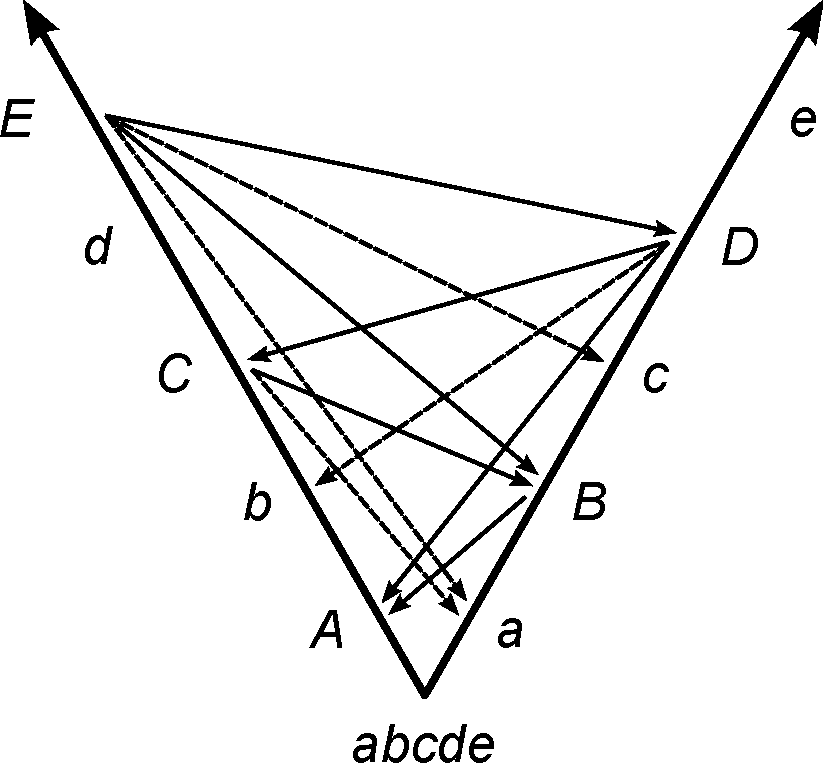
\includegraphics[width=3.5in]{dm-model.pdf}
\end{center}
\caption{\textbf{The Dob\-zhan\-sky-Mul\-ler model of postzygotic isolation.}
%
A population with haploid genotype \emph{abcde} (bottom)
becomes geographically divided into two,
and each population independently evolves through time
(thick arrows, time progresses upward).
%
In the first population,
allele \emph{a} is substituted with allele \emph{A},
while in the second population
allele \emph{b} is substituted with allele \emph{B}.
%
At this point, if the populations were to come into contact and hybridize,
their hybrids would have genotypes
\emph{Abcde}, \emph{aBcde}, or \emph{ABcde}.
%
Because alleles \emph{A} and \emph{B}
evolved independently and thus may only function properly
in the background in which they evolved,
hybrids with genotype \emph{ABcde} may be sterile or inviable.
%
In this case, alleles \emph{A} and \emph{B} are said to form a
Dob\-zhan\-sky-Mul\-ler incompatibility (DMI)
(arrow from \emph{B} to \emph{A}).
%
The populations could have instead hybridized
after two or more alleles have fixed within each lineage
(e.g., alleles \emph{A}, \emph{C}, and \emph{E} in the first population
and alleles \emph{B} and \emph{D} in the second),
which would have resulted in hybrids with many more possible DMIs.
%
DMIs between derived alleles (`derived-derived' DMIs) are thin solid arrows,
and DMIs between derived and ancestral alleles (`derived-ancestral' DMIs)
are thin dashed arrows.
%
(Modified from \citep{orr95}.)}
\label{dm-model}
\end{figure}



% No support for the snowball effect

Several tests of the snowball effect have not supported it
\citep{lij03,men04,gou10}, concluding that there is a `missing snowball.'
%
These tests, however, relied on indirect methods
because testing the snowball effect directly is difficult \citep{men04}.
%
Rather than using a single pair of species and following it through time,
researchers have used different pairs of species diverged at different times
\citep{mal08,sco08}.
%
For the number of DMIs, the strength of postzygotic isolation,
often measured as the reduction in hybrid viability or fertility, has been used.
%
However, for the strength of postzygotic isolation to be a good proxy
for the number of DMIs,
the fitness effects of DMIs on hybrid fitness must be additive
\citep{men04,bol05}
(e.g., twice the number of DMIs should result in twice the isolation),
but whether this is true is not known \citep{bol05,pre10}.



% Support for the snowball effect

Better estimates of the number of DMIs between two species
were recently carried out by two studies \citep{mat10,moy10},
both supporting the snowball effect.
%
To estimate the number of DMIs, they introgressed single genetic regions
of one species into the genetic background of the other and
counted the number of introgressions with reduced viability or fertility.
%
However, this method cannot identify individual DMIs
but rather whether a genetic region of one species
is incompatible with something in the other.
%
As with the previous methods, they relied on the ages of species pairs
rather than following a single species pair through time.
% According to Applied Longitudinal Data Analysis (p. 9), this is bad:
% (http://www.gse.harvard.edu/~faculty/singer/Papers/ch1&2.pdf)
%
In addition, because these studies could only obtain
at most three species pairs with which to count the number of DMIs,
their quadratic fit to the data was not statistically powerful.



% Sample identification of a DMI

To provide an example of what is required to identify a DMI,
suppose that allele $D$ in Fig.~\ref{dm-model} has just fixed
in one population, and we want to test whether it is incompatible
with allele $C$ in the other population.
%
One option is to isolate these alleles in the ancestral genetic background
(\emph{abcde}) to construct the genotype \emph{abCDe} and measure its fitness.
%
In this constructed genotype, however,
alleles $D$ and $b$ as well as alleles $C$ and $a$
may also be incompatible (Fig.~\ref{dm-model}),
and therefore confound the effect of $C$ and $D$ together.
%
Every other possible construction of a genotype that includes $C$ and $D$
(i.e., \emph{aBCDe}, \emph{AbCDe}, and \emph{ABCDe})
also contains other possibly confounding incompatibilities.
%
To prevent these confounding factors, one may only consider
alleles that were compatible with the ancestral background.
%
In the example above, this means that one must first verify that genotypes
\emph{abCde} and \emph{abcDe} had normal fitness before testing \emph{abCDe}.


%- here's what we did
%- here's what we used to do it
%- here's why we used it
%  - accurately count...
%- here's what we got


In this study, we conducted experimental evolution
to test whether pairwise DMIs increased quadratically through time
between evolving populations of digital organisms.
%
We also measured hybrid inviability through time
in order to determine whether there was a missing snowball.
%
Finally, we determined the ratio of derived-derived and derived-ancestral DMIs
and the probability than a pairwise interaction forms a DMI,
which in the literature has been assumed to be constant.
%
We used Avida~\citep{ofr04} (see p. \pageref{sec:avida},
an artificial life research platform,
to conduct our experiments with digital organisms.
%
We used digital organisms for several reasons:
we can observe thousands of generations in minutes,
easily manipulate genomes, which allowed us to
develop a method to accurately count the number of individual pairwise DMIs
as they arose,
and have an accurate historical record.



% I want to end the Introduction with "a brief statement of the overall aim
% of the experiments and a comment about whether that aim was achieved" (PLoS).
% An idea is to move first half of "Science papers" paragraph with
% the paragraph before, then move second half to the end (as a last paragraph)
% and expand more on the results and their significance.

% Need to update fig \ref{avida}B with new epistasis figure (directory try_2)



\section{Results}

To generate the ancestral genotype, we first founded a population
with an organism that could replicate sexually but could not perform any tasks.
%
We then let this population evolve for about 1.5 million generations,
and we took the genotype of the most common organism as the ancestral genotype.
%
Using this ancestor, we then founded 40 independent populations
and allowed them to evolve independently for about 10,000 generations.
%
The configuration parameters, including the environmental conditions,
were the same as those of the ancestor.
%
Every 400 generations, the entire population was saved for later analysis.
%
Because the ancestor was well-adapted to its environment,
the genetic divergence between replicate populations
was mostly due to fixation of neutral mutations.
%
Thus, the rate of substitution for each population
was approximately constant (Fig.~\ref{avida}C),
satisfying an assumption of the snowball effect
when it is analyzed through time \citep{orr95}.
%
The mean relative fitness of hybrids between pairs of populations
at the end of the runs was 0.91 (range: 0.68--0.97) (Fig.~\ref{avida}D),
indicating that incomplete postzygotic isolation had evolved.
%
From now on, we refer to these populations as `species.'



\begin{figure}[p]
\begin{center}
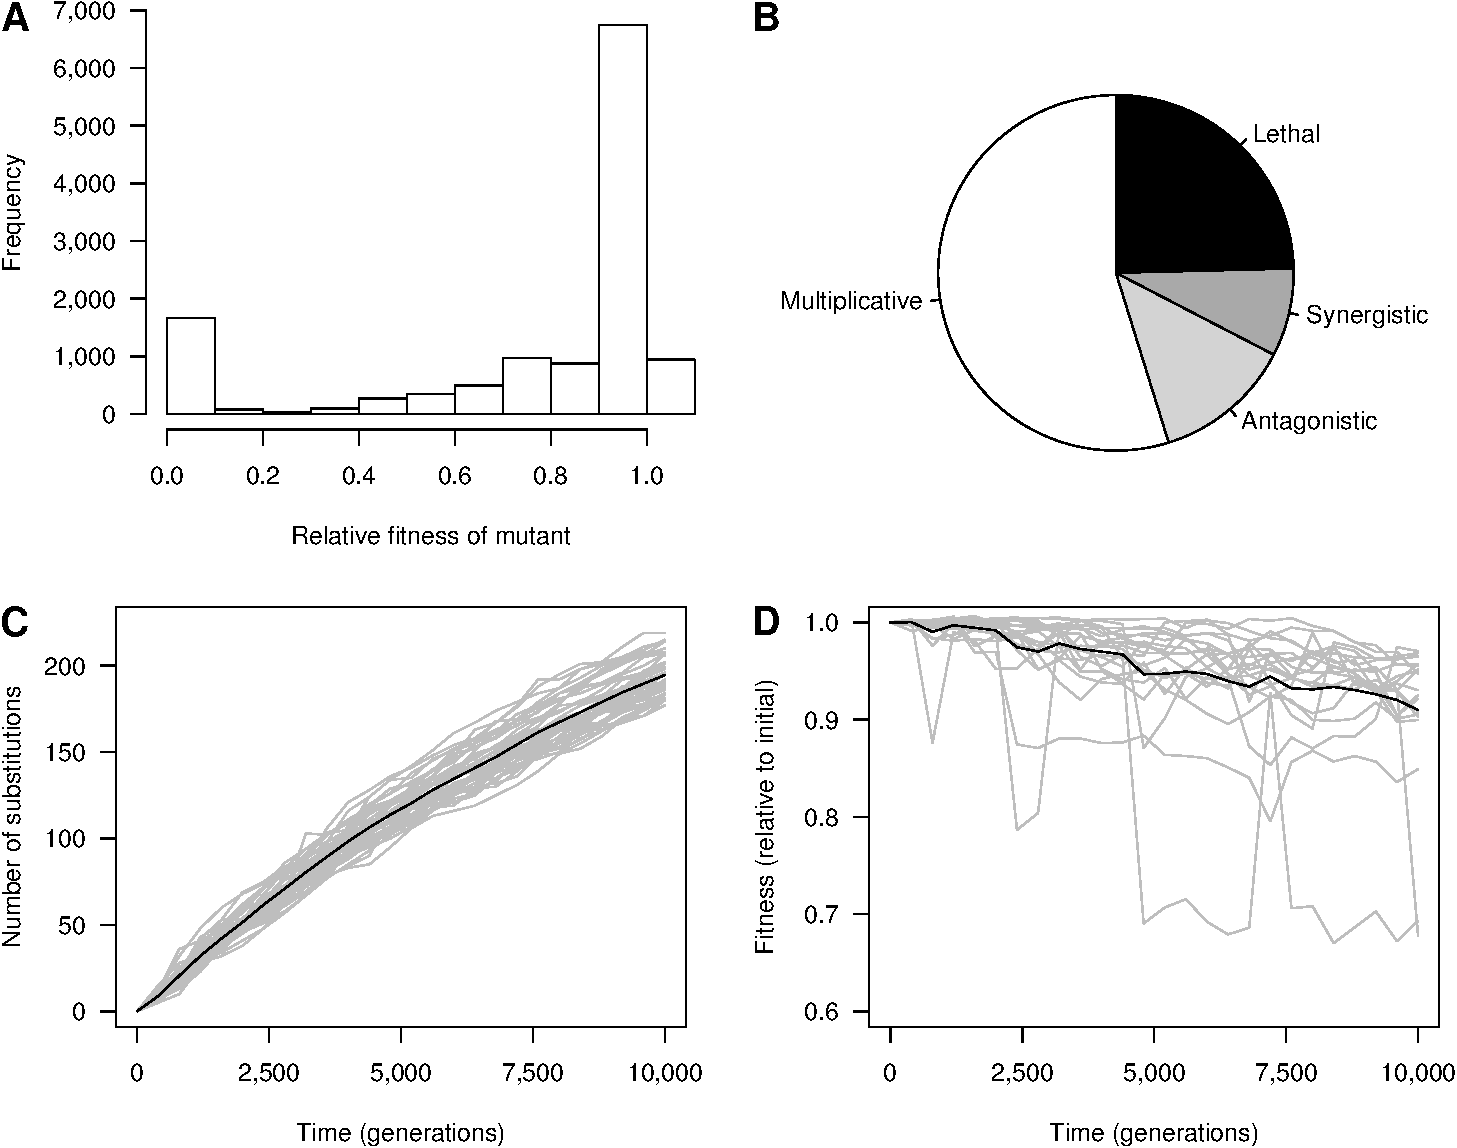
\includegraphics[width=5in]{avida.pdf}
\end{center}
\caption{
  (\textbf{A}) Fitness distribution of all possible single mutants
    of an evolved digital organism.
  (\textbf{B}) Proportions of epistasis types for an evolved digital organism.
  (\textbf{C}) Number of substitutions for each population through time
    (gray lines: individual replicates; black line: mean of replicates).
  (\textbf{D}) Fitness of hybrids between populations through time
    (gray lines: individual replicates; black line: mean of replicates).}
\label{avida}
\end{figure}



\subsection{Pairwise DMIs increased quadratically through time}

To count the number of pairwise DMIs between two species,
we separately counted the number of derived-ancestral
and derived-derived DMIs (Fig.~\ref{dmi-count-method}).
%
To find derived-ancestral DMIs, we first searched
for single derived alleles of each species
that were incompatible with the ancestral background
(e.g., allele~\emph{E} in Fig.~\ref{dmi-count-method}A, step~1).
%
We defined an allele as incompatible with the ancestral background
if the fitness of the ancestral genotype with that allele alone
was $<$~0.75 relative to the original ancestor.
%
To determine whether the incompatibility was due to a single ancestral allele
(thereby forming a derived-ancestral DMI), we searched for another
derived allele of the same species that rescued the incompatibility
(e.g., allele~\emph{C} in Fig.~\ref{dmi-count-method}A, steps~2 and 3).
%
We defined an incompatibly as rescued by another allele if the relative fitness
of the ancestral genotype with both alleles was $>$~0.99.
%
To ensure that the rescue allele was itself not involved in other DMIs,
we verified that its fitness in the ancestral background was also $>$~0.99.
%
We excluded testing rescue alleles that appeared after the derived allele
because in a derived-ancestral DMI a derived allele cannot be incompatible
with any current ancestral alleles (e.g., in Fig.~\ref{dm-model},
allele~\emph{C} cannot be incompatible with \emph{e}).
%
To find derived-derived DMIs, we searched for single derived alleles
from both species that were each compatible with the ancestral background
but together were incompatible (Fig.~\ref{dmi-count-method}B).
%
Using this two-part method, we counted the total number of pairwise DMIs
for each of the 20 replicate pairs of populations every 400 generations.



\begin{figure}[p]
\begin{center}
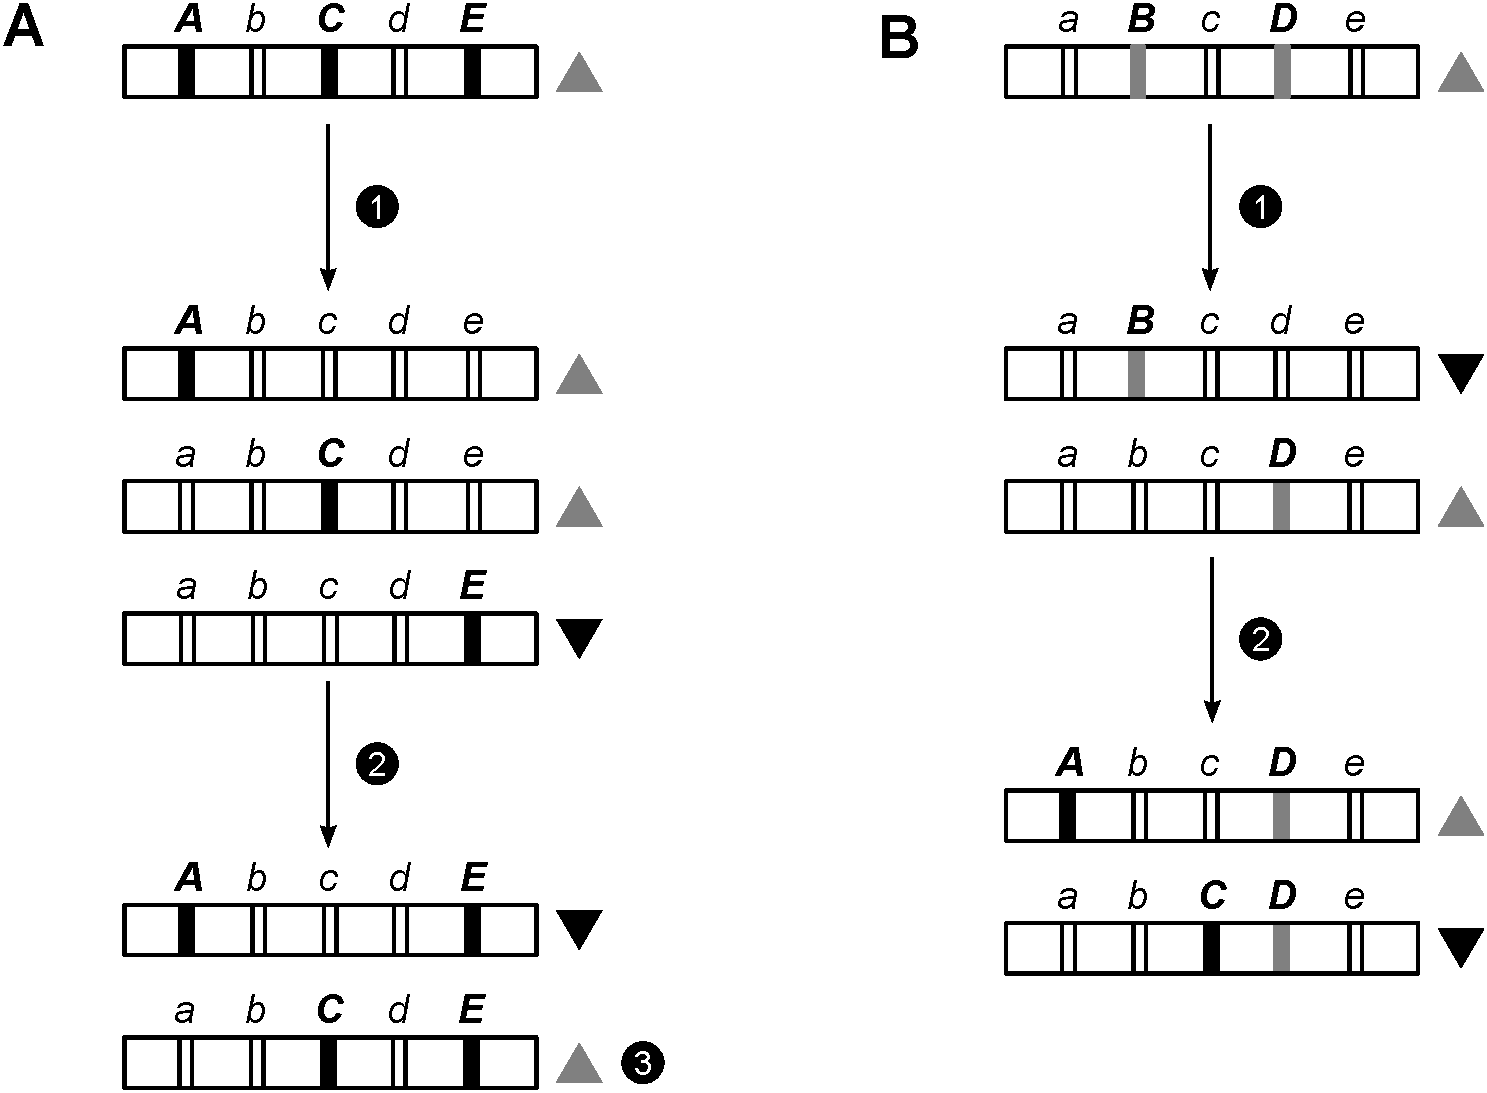
\includegraphics[width=5in]{dmi-count-method.pdf}
\end{center}
\caption{Illustration of the method for identifying
  (\textbf{A}) derived-ancestral
  and (\textbf{B}) derived-derived pairwise DMIs (see text).
  %
  (\textbf{A}) Step 1: We tested the individual fitness effect
  of each derived allele (black bars) of a species on the ancestral background.
  %
  Step 2: For each derived allele that
  was incompatible with the ancestral background
  (indicated by the black triangle pointing down),
  we tested the individual effect of the other derived alleles
  on that genetic background.
  %
  Step 3: If a second derived allele resulted in high fitness
  (indicated by the gray triangle pointing up),
  the ancestral allele at that second locus
  was incompatible with the original derived allele.
  %
  (\textbf{B}) Step 1: We tested the individual fitness effect
  of each derived allele (gray bars) of a species on the ancestral background.
  %
  Step 2: For each derived allele that
  was compatible with the ancestral background,
  we tested the individual effect of each derived allele
  (itself compatible with the ancestral background) of the other species.
  %
  Step 3: If the second allele lowered the fitness,
  then these two allele must be incompatible.}
\label{dmi-count-method}
\end{figure}



To determine whether a linear ($ax$) or a quadratic ($ax^{2} + bx$) model
best described the accumulation of pairwise DMIs through time,
we fit these two models to the whole dataset ($n = 520$)
and to each replicate individually (each $n = 26$).
%
Because there are no pairwise DMIs at the moment of geographic isolation,
the models do not have a constant term (i.e., the intercept is~0).
%
We estimated the parameters of each model using maximum likelihood
with a Gamma distribution for DMIs and compared the models using AIC
\citep{bol08}.
%
We found that the quadratic model explained the whole dataset better
than the linear model (Fig.~\ref{dmi-and-hybrids}A),
although there was considerable variation per replicate
(Fig.~\ref{fig:indiv-dmi}).
%
These results indicate that the overall accumulation of pairwise DMIs
was consistent with the snowball effect.



\begin{figure}
\begin{center}
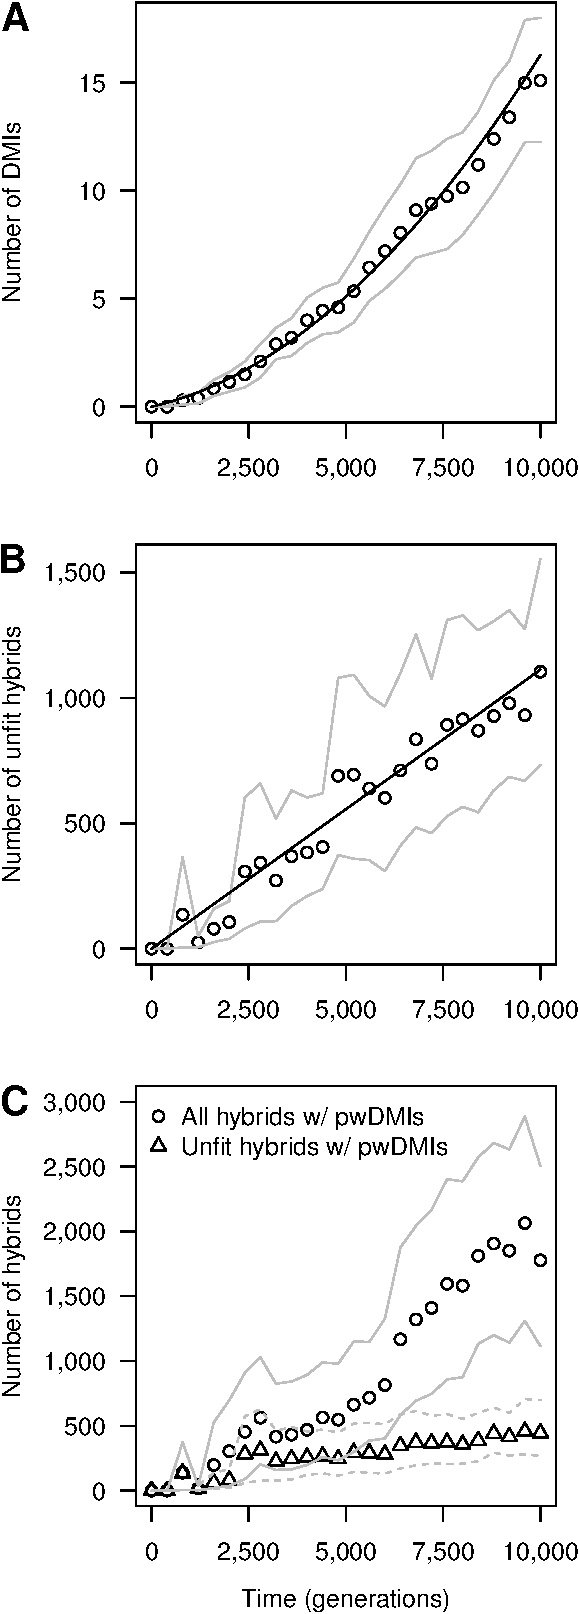
\includegraphics[height=6in]{dmi-and-hybrids.pdf}
\end{center}
\caption{
  (\textbf{A}) Mean number of pairwise DMIs through time.
  Each point represents the mean of 20 replicate runs.
  The black curve represents the quadratic model of the data
  with parameters estimated using maximum likelihood.
  The gray lines represent the bootstrap 95\% confidence intervals of the means.
  %
  (\textbf{B}) Mean number of unfit hybrids (out of 10,000)
  between populations through time.
  Each point represents the mean of 20 replicate runs.
  The black line represents the linear model of the data
  with parameters estimated using maximum likelihood.
  The gray lines represent the bootstrap 95\% confidence intervals of the means.
  %
  (\textbf{C}) Mean number of all hybrids () %find a circle symbol; $\medcirc$)
  and unfit hybrids ($\triangle$) (out of 10,000)
  with at least one pairwise DMI through time.
  Each point represents the mean of 20 replicate runs.
  The gray lines represent the bootstrap 95\%
  confidence intervals of the means.}
\label{dmi-and-hybrids}
\end{figure}



\begin{figure}
\begin{center}
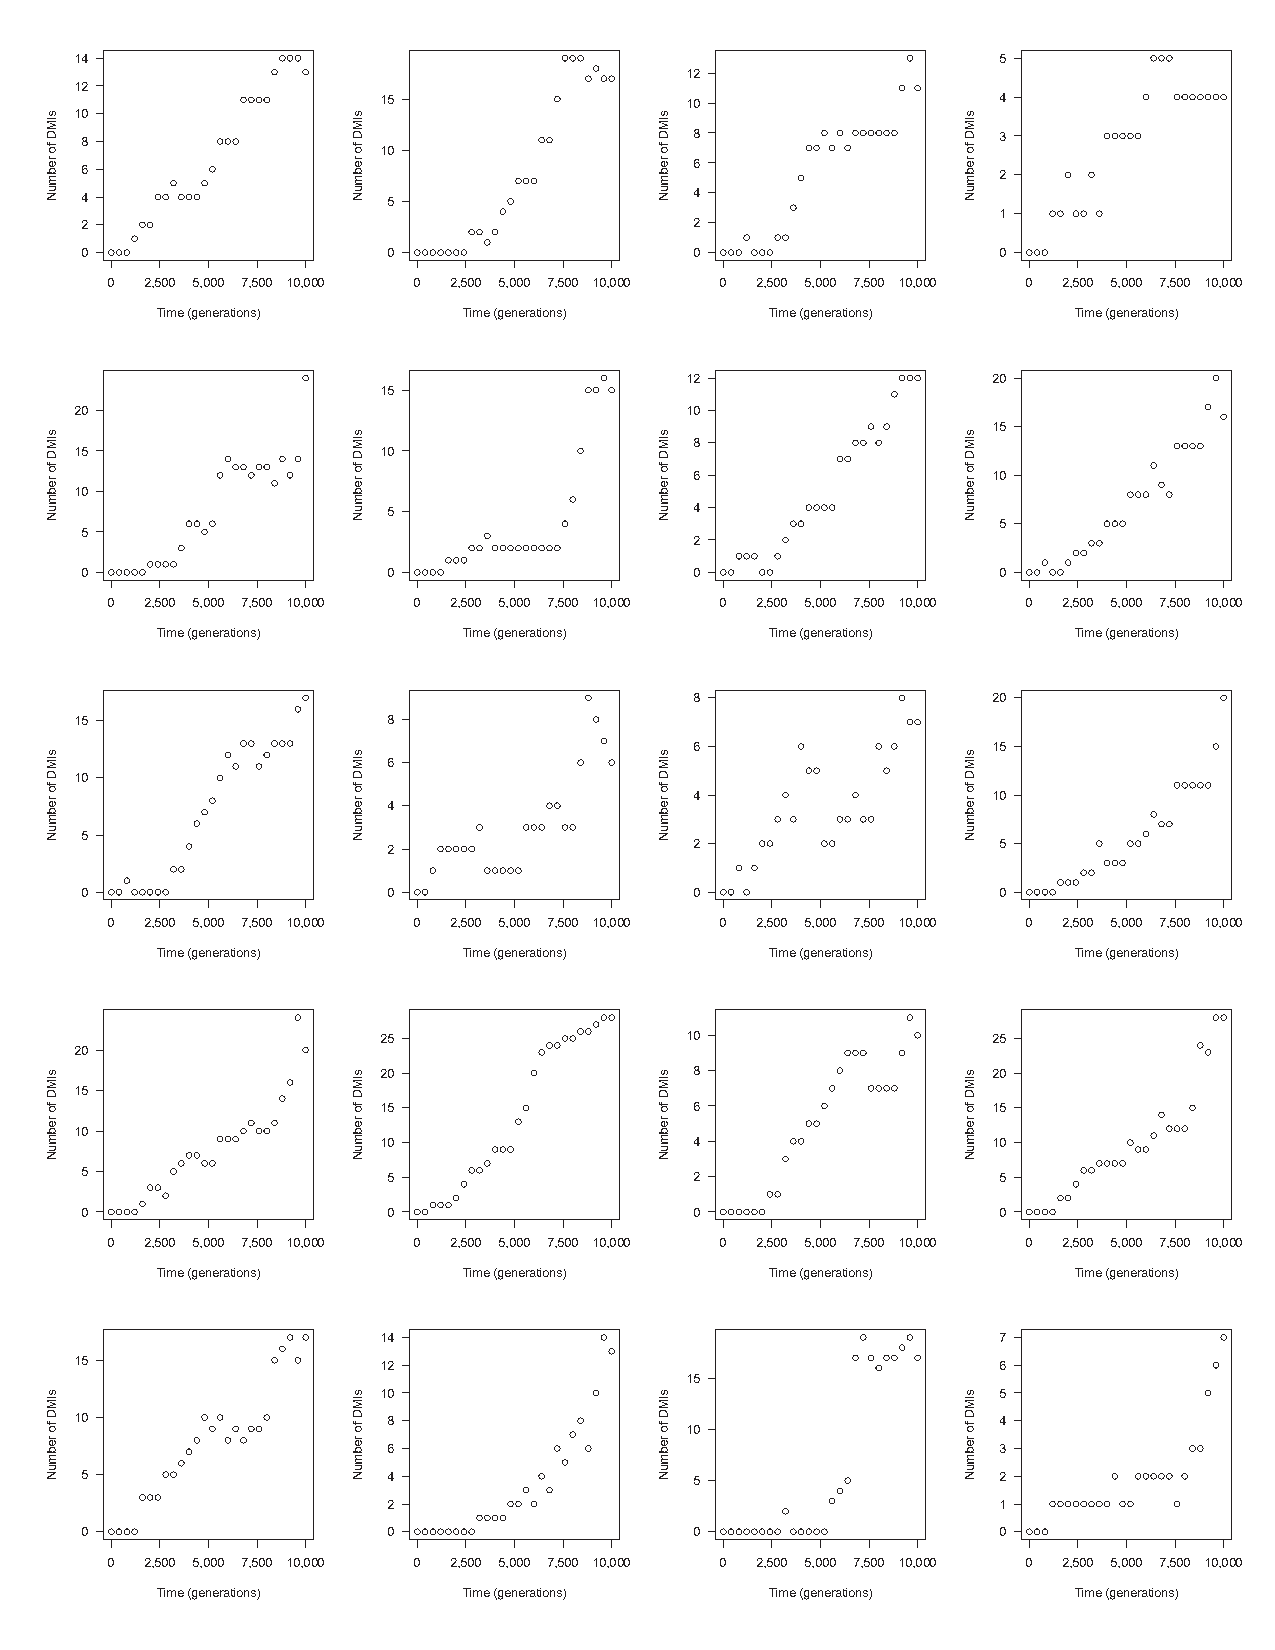
\includegraphics[width=0.9\linewidth]{dmi-counts-indiv-plots.pdf}
\end{center}
\caption{Number of pairwise DMIs through time
  between each replicate pair of populations.}
\label{fig:indiv-dmi}
\end{figure}



\subsection{Hybrid inviability increased linearly through time}

To measure hybrid inviability (i.e., number of unfit hybrids) through time,
we first created 10,000 hybrids between each replicate pair of species
every 400 generations.
%
Hybrids were created in the same way Avida recombines two genotypes:
two random but homologous regions of the parental genomes were exchanged.
%
Note that hybrids were created after the experiments were done,
using the populations we saved every 400 generations;
no hybridization between populations occurred during their evolution.
%
We then measured the fitness of each hybrid and counted the number
(out of 10,000) that had a relative fitness $<$~0.75.
%
We found that the overall number of unfit hybrids through time
increased linearly (Fig.~\ref{dmi-and-hybrids}B),
although there was considerable variation per replicate
(Fig.~\ref{fig:indiv-unfit-hybrids}).
%
These results are consistent with a missing snowball for hybrid inviability
and therefore suggest that the fitness effects of DMIs were not additive.



\begin{figure}
\begin{center}
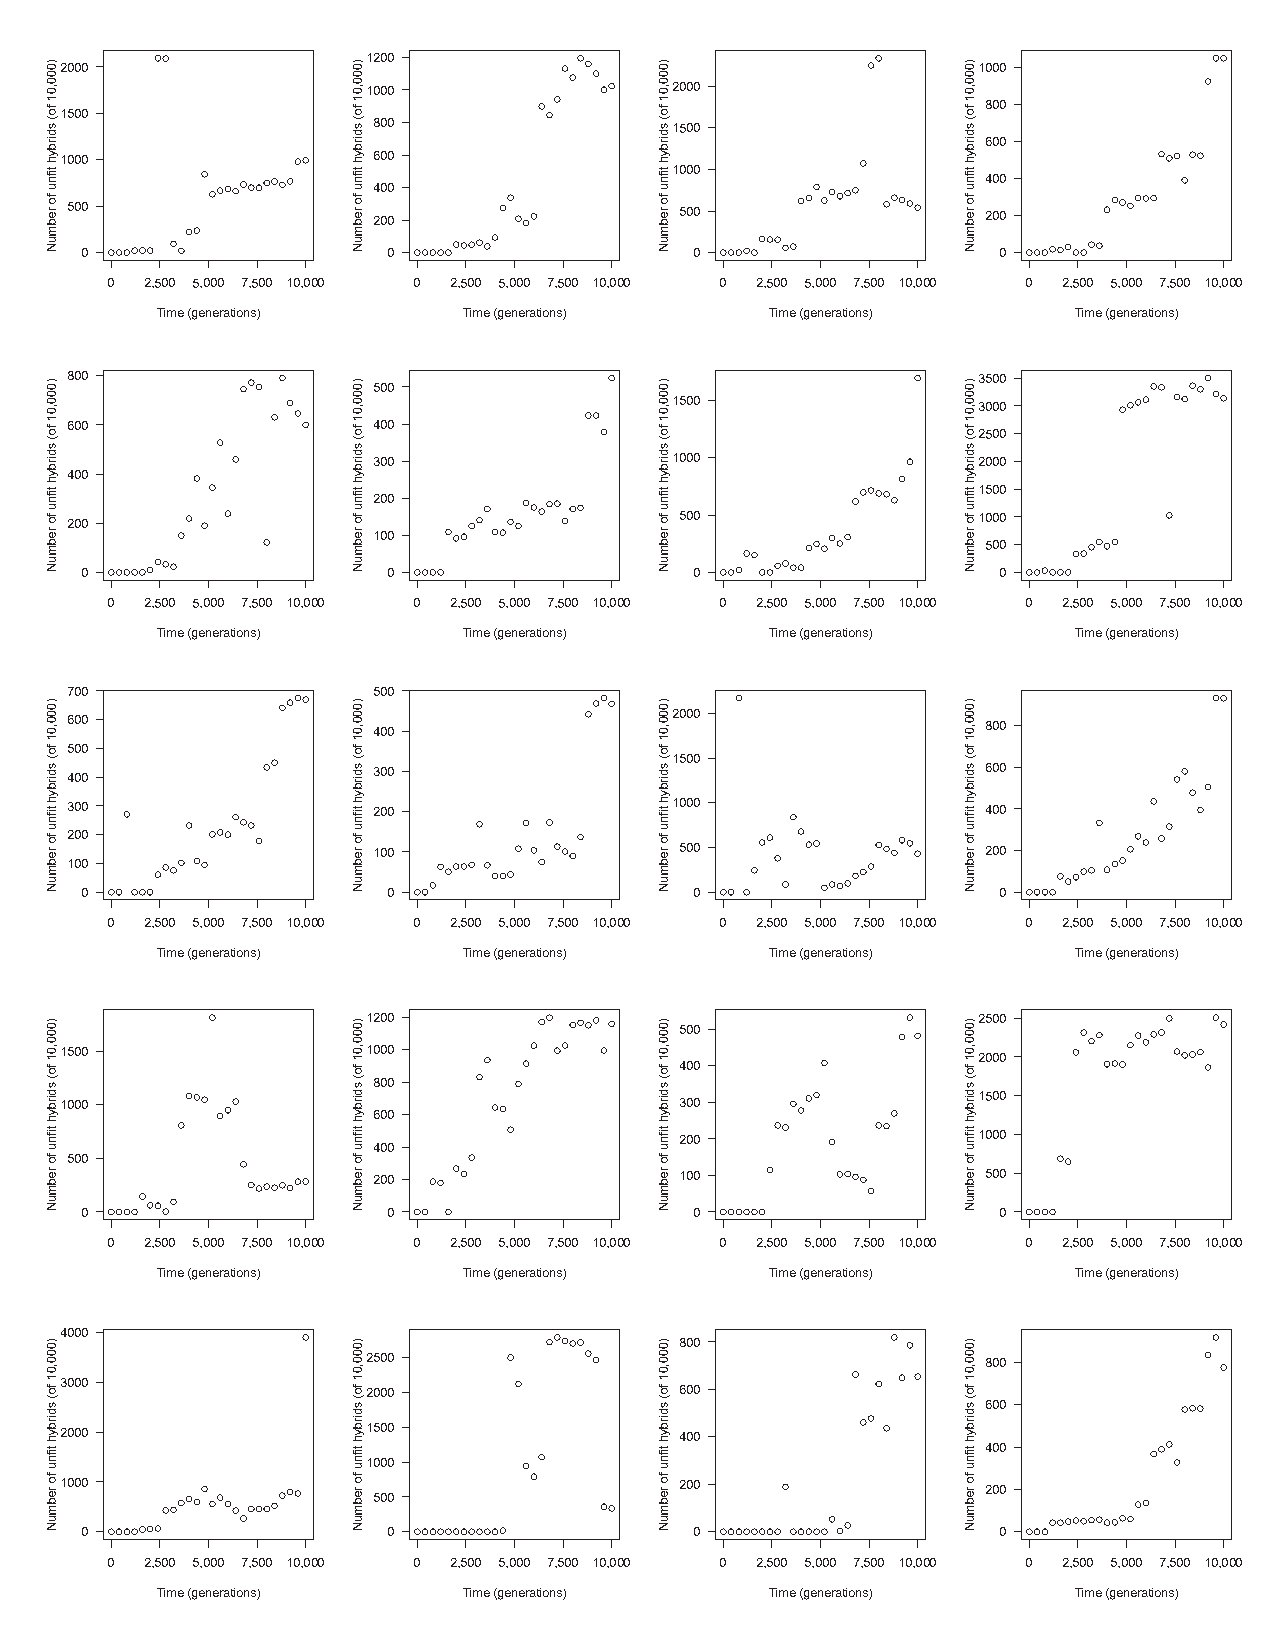
\includegraphics[width=0.9\linewidth]{unfit-hybrid-counts-indiv-plots.pdf}
\end{center}
\caption{Number of unfit hybrids (out of 10,000) through time
  between each replicate pair of populations.}
\label{fig:indiv-unfit-hybrids}
\end{figure}



\subsection{Secondary alleles rescue pairwise DMIs}

%Therefore, we found that in the same experiment
%the mean number of pairwise DMIs increased quadratically,
%while the mean hybrid inviability increased linearly.
Previous studies have found a linear increase
in hybrid inviability through time,
but conclusions that these results indicate the absence
of a snowball effect require that DMIs be additive.
%
If pairwise DMIs were additive, we would expect that hybrids
carrying at least one pairwise DMI be unfit
because a single pairwise DMI should reduce
the fitness of the carrier to $<$ 0.75.
%
We found, however, that not all hybrids
carrying at least one pairwise DMI were unfit
%(e.g., at the end of the runs, only $\sim$ 25\% of such hybrids were unfit)
(Fig. \ref{dmi-and-hybrids}C),
indicating that pairwise DMIs were not additive.
%may interact
%with other derived alleles that rescue the incompatibilities.
% I use 'rescue' to be able to connect it with Drosophila literature
%
One possible reason pairwise DMIs were not additive
is that other derived alleles present in the hybrid rescued pairwise DMIs
(i.e., the true incompatibility was greater than pairwise).
%
This hypothesis predicts that fit hybrids carrying a pairwise DMI
are more likely to carry a rescue allele than unfit hybrids.
%
To test this prediction,
we first identified all possible rescue alleles for all known pairwise DMIs
by searching for single derived alleles from either species
that rescued each known pairwise DMI.
%
Then, for hybrids carrying a pairwise DMI (at generation 10,000),
we calculated the proportion that also carried a rescue allele.
%
We found that 97\% of fit hybrids carried a rescue allele
compared to only 45\% of unfit hybrids.
%
This finding suggests that certain alleles rescued pairwise DMIs,
and this complex interaction could explain
why pairwise DMIs were not additive and therefore
why the mean hybrid inviability increased only linearly.


% Accumulation of DA vs DD DMIs

\subsection{Derived-ancestral DMIs occur as often as derived-derived}

Derived alleles have been predicted to be three times more likely
than ancestral alleles to be involved in pairwise DMIs \citep{orr95}.
%
To test this prediction, we counted the number of times
a derived allele appeared in a DMI
(once in a derived-ancestral DMI and twice in a derived-derived DMI)
and the number of times an ancestral allele appeared in a DMI
(once in a derived-ancestral DMI).
%
We made these counts at 10,000 generations for each pair of populations,
and we calculated the mean of the ratios between the number of derived alleles
and ancestral alleles found in all DMIs.
%
We found that derived alleles are 3.06 (2.41--3.79, 95\% bootstrap C.I.)
times more likely than ancestral alleles to appear in pairwise DMIs,
which experimentally supports the prediction.
%
However, the number of derived-ancestral and derived-derived DMIs
were comparable, suggesting that hybrid inviability due to
a missing dependent allele in the same species was just as likely due to
incompatible derived alleles between species.



\section{Discussion}

% I should say somewhere that the raw numbers of DMIs that form
% in digital organisms should not be taken to reflect biology
% (see review by Presgraves, 2010, AmNat for actual numbers)

% Example where genetics of hybrid sterility is "complex":
% Asymmetry and polymorphism of hybrid male sterility during the early stages of speciation in house mice

Although the mean accumulation of pairwise DMIs increased quadratically,
there was considerable variation in the pattern of accumulation
for individual species pairs (Fig.~S1).
%
There are at least three main possibilities for this variation.
%
First, the probability \emph{p} that two alleles are incompatible
may not be constant through time.
%
For example, a new derived allele may form multiple pairwise incompatibilities
with ancestral or derived alleles of the other population,
increasing the value of \emph{p} temporarily.
%
Second, as an evolving population navigates its neutral landscape,
a derived allele that once caused a DMI may later be replaced
by an allele that does not cause any DMIs.
%
Third, we used the majority-rule consensus sequence
of a population for our analyses,
but alleles in a consensus sequence are not necessarily fixed.
%
For example, an allele that was present in 51\% of the population
would appear in the consensus sequence,
but if that allele later decreases in frequency through drift
it could disappear from the consensus sequence.
%
If such an allele was involved in DMIs,
the estimated number of DMIs would change over time.
%
All of our population pairs underwent evolution
in the same environmental conditions,
yet showed variation in the accumulation of DMIs.
%
This variation suggests that in natural populations,
where environmental conditions between any taxa are rarely identical,
the accumulation of DMIs should also vary considerably.


Alleles that rescue hybrid fitness are not unique to digital organisms.
%
In \emph{Drosophila}, several `hybrid rescue mutations'
recover the viability or fertility
of hybrids between \emph{D. melanogaster} and closely-related species.
%
Note that the \emph{Drosophila} rescue alleles
were artificially selected mutations,
not derived alleles that were fixed in natural populations,
so the importance of rescue alleles in the wild is currently unknown.
%
Two hypotheses explain how rescue alleles
may interact with DMIs.
%
In the first hypothesis, rescue alleles
``suppress the effects of the loci causing hybrid problems'' \citep{coy04}.
%
In this case, rescue alleles may be products of genetic redundancy,
which itself may have evolved as a `buffering mechanism'
against deleterious mutations \citep{wag99,ele06}.
%
For example, a genotype that gains a new allele performing
overlapping functions with another allele at a different locus
will be more robust to deleterious mutations that affect those functions.
%
Although we do not know whether rescue alleles in our system are redundant,
studies have shown that sexual, complex digital organisms
with high mutation rates exhibit mutational robustness \citep{len99,wil01,mis06},
which can evolve by genetic redundancy \citep{ele07}.
%
According to the second hypothesis, rescue alleles
``represent mutations at the actual loci
that cause the death or sterility of hybrids'' \citep{coy04}.
%
This hypothesis implies that hybrid incompatibilities
thought to involve only two alleles actually involve three or more,
as in the case with the hybrid rescue mutation
\emph{Hmr} in \emph{Drosophila} \citep{bar00,orr00}.
%
% EXPLAIN FOLLOWING SENTENCE BETTER (Emily Weigel)
Similarly, if this hypothesis applies
to the rescue alleles we discovered in digital organisms,
then any presumed `pairwise' DMI that was rescued by a third allele
was, in fact, a three-way DMI.
%
Therefore, rescue alleles may provide evidence that complex DMIs,
which are exceptionally difficult to identify in biological organisms,
are common in biological and digital organisms.
% For the above explanation, I'm going to want to invoke
% Maheshwari & Barbash, 2012, which talk about DA DMIs
% possibly being three-way incompatibilities


%Our study reconciles the prediction of a snowball effect
%of the Dob\-zhan\-sky-Mul\-ler model of postzygotic isolation
%with the empirical observation of a ``missing snowball.''
%
In summary, using an artificial life software
we found that pairwise DMIs accumulate quadratically through time,
supporting the snowball effect
and the Dob\-zhan\-sky-Mul\-ler model of postzygotic isolation.
%
In addition, we discovered that the number of derived-ancestral 
and derived-derived DMIs are similar,
suggesting that hybrid inviability due to
a missing allele in the same species
were just as likely due to
incompatible derived alleles between species.
%
When we used the strength of postzygotic isolation
as a proxy for the number of DMIs,
we found a linear, rather than quadratic,
relationship with divergence time.
%
This discrepancy was at least partially caused by rescue alleles,
which we found recovered the negative effects of DMIs in hybrids,
disrupting the pattern of quadratic increase of DMIs.
%
Our findings indicate that pairwise DMIs are insufficient
to account for the complexity of epistatic interactions
among alleles within and between species.
%
Thus, our results highlight the importance of complex interactions
in the genetics of reproductive isolation.

%% Stronger concluding paragraph -- Emily

%I started with how reproductive isolation evolves,
%how has this study helped answer that question?

%RI can evolve through drift



%% FINAL PARAGRAPH
%The effect of selection on the accumulation of DMIs, however,
%remains to be experimentally tested,
%although mathematical models have considered selection \citep{unc09}.
%
%Another interesting thing is
%the effect of gene flow on the accumulation of DMIs,
%providing a genetic mechanism by which isolation is slowed.
%
%Other models have examined the effect of gene flow
%during divergence \citep{kon03}.
%
%Artificial life offers opportunity to study these things empirically.


% Maybe boil down the above to 1 or 2 sentence
% and add to the previous paragraph,
% which itself may be boiled down so it's not too long


% PUT IN METHODS AT THE END
%In Avida, digital organisms consist of a sequence of instructions (or `genome')
%that encodes their ability to replicate and perform computational functions.
%
%Sexual reproduction between two organisms
%exchanges a random but homologous region of their genomes,
%then places the recombinants back into the population.
%
%Organisms are rewarded with a higher replication rate if they evolve
%the ability to perform computational functions,
%which require specific but not unique sequences of instructions.
%
%Variation in the efficiency of replication and in the ability
%to perform functions arises via recombination and mutation.
%
%Because faster replicators in a finite population leave
%more copies of themselves, digital organisms evolve via natural selection
%and genetic drift (i.e., evolution is not simulated).
%
%Fitness, an estimate of an organism's reproductive rate,
%is measured as the amount of rewards obtained divided
%by the number of steps required to replicate.
%
%Although there are many parameters in Avida
%that can be configured (e.g., mutation rate),
%evolutionary processes like natural selection
%and epistasis occur spontaneously.
%
%With Avida, we can
%observe millions of generations of evolution in real-time,
%replicate experiments with identical starting conditions,
%easily manipulate genomes, and
%accurately record measurements
%like fitness and events like mutations.

\section{Methods}

\subsection{Experimental configuration}

The environment was configured to reward the nine default tasks
and 68 additional three-input tasks.
%
All tasks were set to provide a resource value of 1 in an additive fashion;
resources were unlimited.
%
The maximum population size was set to 100 organisms,
and the length of each organism's genome was fixed at 500 instructions.
%
The `copy' mutation probability---the probability that an organism
would copy a random instruction rather than its own to its offspring---%
was set to 0.1 per genome per generation
(all other mutation probabilities were set to 0.0).
%
Mutation to the `h-copy' instruction was turned off to prevent
organisms from using up their genomic space with h-copy instructions
(rather than task-related instructions), which was a common way
to improve their replication efficiency in preliminary runs.
%
Offspring were configured to replace a random organism in the population.



\subsection{Statistics}

Statistical analyses were carried out using R (ver. 2.15.1) \citep{r13}.
%
To perform the AIC analyses, we used the bbmle package \citep{bol08}
and the mle2 function with the `Nelder-Mead' optimization method.
%




\section{Acknowledgments}

We thank A. P. Dreyer, E. M. Swanson, R. E. Lenski, J. W. Boughman,
E. Weigel, E. Dittmar, L. J. Harmon, and D. R. Matute
for helpful comments on the manuscript.
%
This material is based in part upon work supported
by the National Science Foundation under Cooperative Agreement No. DBI-0939454.
Any opinions, findings, and conclusions or recommendations
expressed in this material are those of the author
and do not necessarily reflect the views of the National Science Foundation.



\end{doublespace}

\bibliographystyle{apalike}
\bibliography{snowball}


%%%%%%%    APPENDICES    %%%%%%%%%%
%% If you wish to include one appendix, remove the "%" from the 
%% following two lines.
%\renewcommand{\appname}{APPENDIX}
%\appendix
%% To include several appendices, remove the only the "%"
%% in front of "\appendix".

%% In either cast to start your first appendix, which will be labeled
%% as Appendix A, just type \chapter{<appendix 1 name>}
%% and enter the text of the appendix as you would a chapter.

%%%%%%% A NOTE ABOUT APPENDICES %%%%%%%%%
%% Some appendices may be single spaced such as survey examples or letters.
%% Contact the Graduate School for details.
%% To single space an appendix first remove the % from 
%% the following two lines. 
% \end{doublespace}
% \chapter{<appendix  name>}
%% After entering the appendix remove the % from 
%% the following line
% \begin{doublespace}
%% Any text entered now will be double spaced.
%\end{doublespace}

\end{document}
